% ============================================================================
%  DISSERTATION — Adaptive Symbolic Reasoning and Reinforcement Learning
%                 for Intrusion Detection Systems
% ============================================================================
\documentclass[12pt, letterpaper, oneside]{report}

% ── Packages ────────────────────────────────────────────────────────────────
\usepackage[margin=1in]{geometry}
\usepackage{setspace}
\doublespacing
\usepackage{times}
\usepackage{amsmath, amssymb, amsthm}
\usepackage{algorithm}
\usepackage{algpseudocode}
\usepackage{graphicx}
\usepackage{booktabs}
\usepackage{multirow}
\usepackage{longtable}
\usepackage{tabularx}
\usepackage{caption}
\usepackage{subcaption}
\usepackage{hyperref}
\usepackage{cleveref}
\usepackage{enumitem}
\usepackage{listings}
\usepackage{xcolor}
\usepackage{tikz}
\usetikzlibrary{shapes, arrows.meta, positioning, calc}
\usepackage{pgfplots}
\pgfplotsset{compat=1.18}
\usepackage{tocloft}
\usepackage{fancyhdr}
\usepackage{titlesec}
\usepackage{appendix}
\usepackage{cite}
\graphicspath{{./}}

% ── Page Style ──────────────────────────────────────────────────────────────
\pagestyle{fancy}
\fancyhf{}
\fancyhead[R]{\thepage}
\renewcommand{\headrulewidth}{0pt}

% ── Theorem Environments ────────────────────────────────────────────────────
\newtheorem{definition}{Definition}[chapter]
\newtheorem{theorem}{Theorem}[chapter]
\newtheorem{lemma}[theorem]{Lemma}
\newtheorem{proposition}[theorem]{Proposition}

% ── Custom Commands ─────────────────────────────────────────────────────────
\newcommand{\ASRRL}{\textsc{ASRRL}}
\newcommand{\Qvalue}{Q}
\newcommand{\argmax}{\operatorname*{arg\,max}}
\newcommand{\E}{\mathbb{E}}
\newcommand{\R}{\mathbb{R}}
\newcommand{\N}{\mathbb{N}}
\newcommand{\bx}{\mathbf{x}}
\newcommand{\bs}{\mathbf{s}}

% ============================================================================
%  TITLE PAGE
% ============================================================================
\begin{document}

\begin{titlepage}
\centering
\vspace*{1in}

{\Large\bfseries ADAPTIVE SYMBOLIC REASONING AND REINFORCEMENT LEARNING\\
FOR INTRUSION DETECTION SYSTEMS:\\
A FORMALLY VERIFIABLE FRAMEWORK WITH\\
ONLINE NOVEL ATTACK DETECTION}

\vspace{1.5in}

{\large A Dissertation\\
Presented to the Faculty of the Graduate School\\
in Partial Fulfillment of the Requirements\\
for the Degree of\\[0.5em]
\textbf{Doctor of Philosophy in Computer Science}}

\vspace{1.5in}

{\large by\\[0.5em]
\textbf{Palmer Young}}

\vspace{1.5in}

{\large 2026}

\end{titlepage}

% ── Copyright Page ──────────────────────────────────────────────────────────
\thispagestyle{empty}
\vspace*{\fill}
\begin{center}
\copyright\ 2026 Palmer Young\\
All Rights Reserved
\end{center}
\vspace*{\fill}
\clearpage

% ── Abstract ────────────────────────────────────────────────────────────────
\pagenumbering{roman}
\setcounter{page}{3}

\chapter*{Abstract}
\addcontentsline{toc}{chapter}{Abstract}

Modern network intrusion detection systems (IDS) face a fundamental tension between detection accuracy and operational trustworthiness: machine learning classifiers achieve high accuracy but produce opaque, unverifiable decisions, while rule-based systems offer transparency but cannot adapt to novel threats. This dissertation introduces the \emph{Adaptive Symbolic Reasoning and Reinforcement Learning} (\ASRRL{}) framework, a Adaptive Symbolic-RL Pipeline that unifies decision tree classification, Z3 Satisfiability Modulo Theories (SMT) constraint verification, Q-learning with an epsilon-greedy policy, and DBSCAN-based online novel attack detection into a single, formally verifiable intrusion detection system.

The \ASRRL{} framework makes five principal contributions. First, it introduces a \emph{novel Adaptive Symbolic-RL formally verifiable IDS architecture} with a \emph{symbolic safety shield} that extracts decision tree paths as first-order logic constraints, encodes them in the Z3 SMT solver, and formally verifies every reinforcement learning action \emph{before execution}, guaranteeing that no classification violates learned safety invariants. Second, it proposes an \emph{online novel attack detector} that applies DBSCAN clustering to misclassified network flows in a rolling buffer, identifies previously unseen attack patterns without retraining, and automatically converts discovered cluster centers into new Z3 constraints, enabling zero-day adaptation. Third, it introduces a \emph{dynamic buffer and threshold adaptation} mechanism that adjusts buffer sizing based on observed feature variance and adapts the classification threshold based on the running FPR-to-FNR ratio, enabling the system to maintain stable performance under varying attack intensities without manual parameter tuning. Fourth, it demonstrates \emph{competitive accuracy with full formal verifiability}, achieving F1 scores of $0.9459$--$0.9995$ while maintaining 100\% constraint coverage and decision traceability. Fifth, it defines a \emph{Composite Verifiability Score} (CVS) comprising seven sub-metrics that quantify the formal auditability of IDS decisions for deployment in critical infrastructure.

Experimental evaluation across four benchmark datasets (UNSW-NB15, CSE-CIC-IDS-2018, CIC-IDS2017, and MISP ThreatFox threat intelligence) demonstrates that \ASRRL{} achieves F1 scores of $0.9459$--$0.9995$ while maintaining a CVS of $0.9523$--$0.9626$, compared to $0.21$--$0.28$ for baseline classifiers (SVM, KNN, Naive Bayes, MLP), which \ASRRL{} outperforms on both accuracy and verifiability. In the novel attack experiment with temporally phased holdout attacks, \ASRRL{} discovers up to 385 novel attack patterns online and sustains adaptive F1 scores across three deployment phases, while static baselines show no adaptation capability. Statistical significance is confirmed via Wilcoxon signed-rank tests ($p < 0.005$) against all evaluated baselines.

\textbf{Keywords:} intrusion detection, reinforcement learning, symbolic reasoning, Z3 SMT solver, DBSCAN, novel attack detection, formal verification, explainable AI, network security.

% ── Acknowledgments ─────────────────────────────────────────────────────────
\chapter*{Acknowledgments}
\addcontentsline{toc}{chapter}{Acknowledgments}

\emph{[To be completed by the author.]}

% ── Table of Contents ───────────────────────────────────────────────────────
\tableofcontents
\listoffigures
\listoftables
\clearpage

% ── List of Abbreviations ──────────────────────────────────────────────────
\chapter*{List of Abbreviations}
\addcontentsline{toc}{chapter}{List of Abbreviations}

\begin{tabular}{@{}ll@{}}
\toprule
\textbf{Abbreviation} & \textbf{Definition} \\
\midrule
ASRRL & Adaptive Symbolic Reasoning and Reinforcement Learning \\
CVS & Composite Verifiability Score \\
DBSCAN & Density-Based Spatial Clustering of Applications with Noise \\
DT & Decision Tree \\
FNR & False Negative Rate \\
FPR & False Positive Rate \\
IDS & Intrusion Detection System \\
IOC & Indicator of Compromise \\
KNN & $k$-Nearest Neighbors \\
MCP & Model Context Protocol \\
MISP & Malware Information Sharing Platform \\
MLP & Multi-Layer Perceptron \\
NIDS & Network Intrusion Detection System \\
RL & Reinforcement Learning \\
SMT & Satisfiability Modulo Theories \\
SOC & Security Operations Center \\
SVM & Support Vector Machine \\
XGB & XGBoost (Extreme Gradient Boosting) \\
\bottomrule
\end{tabular}

% ============================================================================
%  CHAPTER 1 — INTRODUCTION
% ============================================================================
\pagenumbering{arabic}
\setcounter{page}{1}

\chapter{Introduction}
\label{ch:introduction}

\section{Background and Context}
\label{sec:background}

The proliferation of networked systems across critical infrastructure, cloud computing, and Internet of Things (IoT) environments has expanded the attack surface available to adversaries. According to recent industry reports, the global cost of cybercrime is projected to exceed \$10.5 trillion annually by 2025~\cite{barbero2022}, with network intrusions constituting one of the most prevalent and damaging attack vectors. Network Intrusion Detection Systems (NIDS) serve as a foundational defense layer, monitoring network traffic flows and classifying them as benign or malicious in real time.

Historically, NIDS have followed two distinct paradigms. \emph{Signature-based} systems, exemplified by Snort~\cite{roesch1999} and Suricata, match observed traffic against a database of known attack patterns. While highly precise for known threats, these systems are unable to detect novel attacks, which is a notable limitation given that adversaries continuously develop new techniques, tactics, and procedures (TTPs). \emph{Anomaly-based} systems, by contrast, learn a model of normal behavior and flag deviations. Machine learning approaches have dominated this paradigm for over a decade~\cite{buczak2016}, with Random Forests, Support Vector Machines, and deep neural networks achieving F1 scores exceeding 0.99 on standard benchmarks such as UNSW-NB15~\cite{moustafa2015} and CIC-IDS2017~\cite{sharafaldin2018}.

Despite these reported benchmark results, the deployment of ML-based IDS in production environments remains limited by three interrelated challenges. The first is \emph{opacity}: black-box classifiers produce predictions without explanations, leaving security analysts unable to determine \emph{why} a flow was classified as an attack (which features contributed, which rules were triggered, or whether the decision is consistent with organizational security policy). This opacity undermines trust and impedes regulatory compliance, particularly in sectors governed by frameworks such as NIST SP 800-53 and the EU AI Act~\cite{buczak2016}.

The second challenge is \emph{static decision boundaries}. Supervised classifiers are trained on a fixed dataset and deployed with frozen parameters. When adversaries introduce novel attack types (zero-day exploits, new malware families, or evolved command-and-control (C2) protocols), the classifier cannot adapt without costly offline retraining, data re-collection, and model re-validation~\cite{jordaney2017}. This rigidity creates a persistent window of vulnerability between the emergence of a new attack and the deployment of an updated model.

The third challenge is the \emph{absence of formal safety guarantees}. No mainstream ML-based IDS provides a mechanism to \emph{prove} that its decisions satisfy a set of safety constraints. A classifier might achieve 99\% accuracy overall yet systematically misclassify a specific attack variant that happens to fall near the decision boundary. Without formal verification, such failure modes are undetectable until exploitation occurs~\cite{alshiekh2018}.

Addressing these three challenges requires drawing on several foundational techniques from machine learning, formal methods, and data mining, which are briefly introduced here and developed in detail in Chapters~\ref{ch:literature} and~\ref{ch:methodology}.

\emph{Machine learning for intrusion detection} encompasses a family of computational methods that learn patterns from labeled network traffic data to distinguish benign flows from attacks. Common approaches include decision trees, which partition the feature space through a sequence of threshold-based splits; ensemble methods such as Random Forests and gradient boosting (XGBoost, LightGBM), which combine multiple weak learners to improve accuracy; and neural network architectures including multi-layer perceptrons (MLPs), convolutional neural networks (CNNs), and recurrent networks (LSTMs). While these methods achieve high accuracy, they typically produce opaque decisions that cannot be formally audited.

\emph{Reinforcement learning} (RL) is a paradigm in which an agent learns to make sequential decisions by interacting with an environment and receiving reward signals. In the IDS context, the agent observes a network flow (the state), selects a classification action (ALLOW, BLOCK, or UNKNOWN), and receives a reward based on whether the classification was correct. Q-learning, a foundational RL algorithm, maintains a table of expected cumulative rewards for each state-action pair and updates these values as the agent gains experience. An epsilon-greedy exploration policy balances the agent's tendency to exploit known good actions with the need to explore potentially better alternatives.

\emph{Satisfiability Modulo Theories} (SMT) solving is a formal verification technique that determines whether a set of logical constraints over mathematical theories (e.g., real arithmetic, bit-vectors) can be simultaneously satisfied. The Z3 solver, developed by Microsoft Research~\cite{demoura2008}, is a widely used SMT solver that can check whether a proposed classification action is consistent with a set of formally encoded rules. In the context of this dissertation, decision tree paths (sequences of feature-threshold comparisons leading from root to leaf) are extracted and encoded as first-order logic constraints in Z3, enabling formal verification of every classification decision before execution.

\emph{Density-Based Spatial Clustering of Applications with Noise} (DBSCAN) is an unsupervised clustering algorithm that groups data points based on density reachability~\cite{ester1996}. Unlike $k$-means, DBSCAN does not require specifying the number of clusters in advance and can discover clusters of arbitrary shape while identifying outliers as noise. In IDS applications, DBSCAN can be applied to collections of misclassified network flows to discover dense clusters that may represent previously unseen attack types.

\emph{Adversarial perturbation} refers to the deliberate modification of input features to cause a classifier to produce incorrect predictions. In network security, adversaries may craft traffic flows with slightly altered characteristics to evade detection. \emph{Concept drift} occurs when the statistical properties of attack traffic change over time; for example, when adversaries modify their tactics, techniques, and procedures (TTPs), causing classifiers trained on historical data to degrade in performance.

Finally, \emph{dynamic buffer and threshold mechanisms} are adaptive control strategies that adjust system parameters in response to observed performance. A dynamic buffer adjusts its size based on observed feature variance to balance between responsiveness (smaller buffer) and statistical reliability (larger buffer). A dynamic classification threshold adjusts the decision boundary based on the running ratio of false positive rate (FPR) to false negative rate (FNR), maintaining an appropriate balance between detection sensitivity and false alarm rate without manual tuning.


\section{Purpose of the Study}
\label{sec:purpose}

This dissertation addresses the three challenges identified above (opacity, static decision boundaries, and absence of formal safety guarantees) through the \emph{Adaptive Symbolic Reasoning and Reinforcement Learning} (\ASRRL{}) framework.

The \ASRRL{} framework is a unified intrusion detection architecture that combines four complementary techniques into a single classification pipeline. At its core, a balanced decision tree classifier provides initial predictions and serves as the source of interpretable symbolic constraints. The paths through the decision tree, each a sequence of feature-threshold comparisons leading to a classification, are extracted and encoded as first-order logic formulas in the Z3 SMT solver, forming a \emph{symbolic safety shield}. A tabular Q-learning agent then learns an action-value function over the decision tree's leaf-based state space, selecting classification actions that are verified against the Z3 constraint set before execution. When the agent's proposed action fails verification, the safety shield overrides with the highest-value verified alternative, ensuring that no classification violates the learned safety invariants. Finally, a DBSCAN-based novel attack detector monitors misclassified flows in a rolling Novelty Candidate Buffer, discovers dense clusters representing previously unseen attack patterns, and automatically converts discovered cluster centroids into new Z3 constraints, enabling the system to adapt to zero-day attacks without offline retraining.

What distinguishes \ASRRL{} from prior work is the tight integration of these components: the decision tree provides the interpretable bridge between subsymbolic learning (RL Q-values) and symbolic reasoning (Z3 constraints), while the DBSCAN feedback loop ensures that the symbolic knowledge base grows continuously in response to novel threats. This architecture achieves formal verifiability, online adaptability, and competitive detection accuracy simultaneously, properties that existing IDS frameworks treat as mutually exclusive.


\section{Research Problem}
\label{sec:research_problem}

The central research problem addressed by this dissertation is the design, implementation, and empirical validation of a network intrusion detection system that simultaneously achieves (a)~competitive detection accuracy relative to state-of-the-art classifiers, (b)~formal verifiability of every classification decision via symbolic constraint satisfaction, and (c)~adaptation to previously unseen attack types during deployment without offline retraining.

This problem is non-trivial because the three objectives are traditionally in tension. High-accuracy models (e.g., deep neural networks) sacrifice interpretability and verifiability. Formally verifiable systems (e.g., rule-based expert systems) sacrifice adaptability. Online learning algorithms (e.g., incremental clustering) sacrifice the structured decision-making needed for formal guarantees. The \ASRRL{} framework addresses these tensions by layering complementary techniques, each handling a distinct objective, into a coherent Adaptive Symbolic-RL Pipeline.


\section{Research Questions}
\label{sec:research_questions}

This dissertation is guided by the following research questions:

\begin{enumerate}[label=\textbf{RQ\arabic*.}]
    \item Does the \ASRRL{} framework achieve detection accuracy (measured by F1 score, precision, recall, FPR, and FNR) that is statistically superior to established baseline classifiers (SVM, KNN, Naive Bayes, MLP) across multiple benchmark datasets?

    \item Can Z3 SMT constraints extracted from decision tree paths and DBSCAN-detected novel patterns provide meaningful formal verification of reinforcement learning actions, as measured by constraint coverage, decision traceability, and the Composite Verifiability Score (CVS)?

    \item Does the DBSCAN-based novel pattern detector enable \ASRRL{} to adapt to previously unseen attack types during deployment, and does this adaptation measurably improve detection performance relative to static baselines in a temporally phased evaluation?

    \item How does \ASRRL{} perform under adversarial feature perturbations and simulated concept drift compared to baseline classifiers?

    \item Does the dynamic buffer and threshold mechanism enable \ASRRL{} to maintain stable performance across varying attack intensities without manual parameter tuning?
\end{enumerate}


\section{Study Goals and Objectives}
\label{sec:study_goals}

The overarching goal of this research is to design, implement, and empirically evaluate a network intrusion detection framework that bridges the gap between machine learning accuracy and formal verification guarantees. Specific objectives include:

\begin{enumerate}[label=\textbf{O\arabic*.}]
    \item Design a Adaptive Symbolic-RL classification pipeline that integrates decision trees, Z3 SMT constraints, Q-learning, and DBSCAN clustering.
    \item Implement the symbolic safety shield that extracts decision tree paths as first-order logic constraints and verifies every RL action before execution.
    \item Develop the online novel attack detector that identifies previously unseen attack clusters from misclassified flows and converts them to Z3 constraints in real time.
    \item Define the Composite Verifiability Score (CVS) as a multi-dimensional metric for assessing the formal auditability of IDS decisions.
    \item Evaluate \ASRRL{} against four baseline classifiers across four benchmark datasets using nine evaluation dimensions.
    \item Demonstrate online adaptation capability through a temporally phased novel attack experiment with holdout attack types.
    \item Validate statistical significance of results using Wilcoxon signed-rank and Mann-Whitney U tests.
\end{enumerate}


\section{Theoretical Framework}
\label{sec:theoretical_framework}

The \ASRRL{} framework draws on four theoretical foundations:

\subsection{Reinforcement Learning Theory}

The classification task is modeled as a Markov Decision Process (MDP) $\mathcal{M} = (\mathcal{S}, \mathcal{A}, P, R, \gamma)$, where:
\begin{itemize}
    \item $\mathcal{S}$: State space, consisting of discretized network flow feature vectors $\bs \in \R^{10}$.
    \item $\mathcal{A} = \{\texttt{ALLOW}, \texttt{BLOCK}, \texttt{UNKNOWN}\}$: Action space with three classification decisions.
    \item $P$: Transition probability, defined by the sequence of incoming flows.
    \item $R: \mathcal{S} \times \mathcal{A} \rightarrow \R$: Reward function with asymmetric penalties (Section~\ref{sec:reward_function}).
    \item $\gamma = 0.90$: Discount factor balancing immediate and future rewards.
\end{itemize}

The agent learns an action-value function $Q: \mathcal{S} \times \mathcal{A} \rightarrow \R$ via the Q-learning update rule:
\begin{equation}
\label{eq:qlearning}
Q(s_t, a_t) \leftarrow Q(s_t, a_t) + \alpha \left[ r_t + \gamma \max_{a'} Q(s_{t+1}, a') - Q(s_t, a_t) \right]
\end{equation}
where $\alpha = 0.10$ is the learning rate.

\subsection{Satisfiability Modulo Theories (SMT)}

Z3 is an SMT solver developed by Microsoft Research that decides the satisfiability of first-order logic formulas over combinations of theories (arithmetic, arrays, bit-vectors). In \ASRRL{}, each decision tree path from root to leaf is encoded as a conjunction of feature predicates:
\begin{equation}
\label{eq:z3constraint}
\phi_k = \bigwedge_{i=1}^{d_k} \left( x_{f_i} \leq \theta_i \lor x_{f_i} > \theta_i \right) \implies a_k
\end{equation}
where $d_k$ is the depth of path $k$, $f_i$ is the feature index at split $i$, $\theta_i$ is the threshold, and $a_k \in \mathcal{A}$ is the leaf action. The Z3 solver verifies whether a proposed RL action is consistent with the full constraint set $\Phi = \{\phi_1, \ldots, \phi_K\}$.

\subsection{Density-Based Clustering}

DBSCAN (Density-Based Spatial Clustering of Applications with Noise) groups data points by density reachability. Given parameters $\varepsilon$ (neighborhood radius) and \texttt{min\_samples} (minimum cluster size), DBSCAN identifies core points, border points, and noise without requiring a pre-specified number of clusters. In \ASRRL{}, DBSCAN is applied to the rolling buffer of misclassified flows to discover novel attack clusters.

\subsection{Formal Verification in Safety-Critical Systems}

The safety shield concept draws on the \emph{shielded reinforcement learning} paradigm, where a formal monitor constrains an RL agent's action space to prevent safety violations. In \ASRRL{}, the Z3 constraint set acts as the shield: if the agent's proposed action fails verification, the shield selects the highest-Q-value action that satisfies all constraints.


\section{Significance of the Study and Contributions}
\label{sec:significance}

This research makes the following principal contributions to the fields of network security and machine learning:

\begin{enumerate}
    \item \textbf{A Novel Formally Verifiable IDS Architecture.} \ASRRL{} is, to the best of our knowledge, the first IDS framework that integrates decision tree classification, Z3 SMT constraint verification, tabular Q-learning, and DBSCAN novel pattern detection into a single, formally verifiable pipeline. Every classification action is verified against a formally derived constraint set before execution, achieving a Composite Verifiability Score of 0.960, compared to 0.16--0.23 for all baseline classifiers.

    \item \textbf{Online Novel Attack Detection via DBSCAN-to-Z3 Constraint Injection.} The framework introduces a closed-loop mechanism in which misclassified flows are accumulated in a rolling buffer, clustered by DBSCAN to discover novel attack patterns, and automatically converted to Z3 constraints injected into the safety shield in real time. This enables zero-day adaptation without offline retraining. Across four datasets, \ASRRL{} discovers up to 385 novel patterns and sustains F1 performance across all temporal phases.

    \item \textbf{Dynamic Buffer and Threshold Adaptation.} The framework contributes an adaptive buffer sizing and threshold adjustment mechanism that responds to changing attack distributions in real time. The buffer contracts under high feature variance and expands under stable conditions, while the classification threshold adjusts based on the running FPR-to-FNR ratio. The fully dynamic configuration achieves the highest F1 and lowest FPR compared to all fixed-parameter alternatives.

    \item \textbf{Competitive Accuracy with Full Formal Verifiability.} \ASRRL{} achieves F1 scores of 0.9459--0.9995 across four benchmark datasets while maintaining 100\% constraint coverage, 100\% decision traceability, and 100\% safety guarantee, demonstrating that the traditional trade-off between accuracy and interpretability can be mitigated.

    \item \textbf{Composite Verifiability Score (CVS) Metric.} This dissertation proposes a novel seven-dimensional metric for quantifying the formal auditability of an IDS, encompassing rule extractability, constraint coverage, decision traceability, safety guarantee, deterministic reproducibility, audit trail completeness, and explanation complexity. The CVS provides a standardized basis for comparing the trustworthiness of IDS approaches and for demonstrating compliance with regulatory requirements.
\end{enumerate}


\section{Scope and Limitations}
\label{sec:limitations}

The following limitations bound the scope of this work:

\begin{enumerate}
    \item \textbf{Binary classification focus.} The primary evaluation uses binary classification (benign vs.\ attack). Multi-class attack categorization is evaluated as a secondary dimension but is not the central contribution.

    \item \textbf{Flow-level features.} \ASRRL{} operates on a standardized set of 10 flow-level features. Payload inspection, application-layer protocol analysis, and raw packet-level features are outside the scope.

    \item \textbf{Tabular Q-learning.} The RL agent uses tabular Q-learning with decision-tree-leaf-based state discretization. Deep reinforcement learning variants (DQN, PPO, A3C) are left as future work.

    \item \textbf{Adversarial robustness.} While Gaussian perturbation experiments are conducted, sophisticated adversarial attacks (e.g., gradient-based evasion targeting the decision tree or RL policy) are not fully explored.

    \item \textbf{Deployment context.} The framework is evaluated in an offline simulation environment with temporal phasing. Real-time deployment at line rate on production networks is discussed as future work.

    \item \textbf{MISP data augmentation.} The MISP ThreatFox dataset consists of threat intelligence IOCs rather than full packet captures; synthetic benign traffic is augmented at a 65\% ratio to enable binary classification evaluation.
\end{enumerate}


\section{Key Terminology}
\label{sec:terminology}

\begin{definition}[Network Flow]
A network flow is a sequence of packets sharing a common 5-tuple: source IP, destination IP, source port, destination port, and transport protocol~\cite{lee1998}. Flows are characterized by aggregate statistics including duration, packet rate, byte rate, and inter-arrival time variability.
\end{definition}

\begin{definition}[Symbolic Safety Shield]
A formal verification mechanism that constrains the reinforcement learning agent's action space by encoding decision tree paths and DBSCAN-detected novel patterns as Z3 SMT constraints~\cite{demoura2008, alshiekh2018}. Before any classification action is executed, the shield verifies that the action satisfies all constraints; if verification fails, the shield overrides the agent's decision with a safe alternative.
\end{definition}

\begin{definition}[Composite Verifiability Score (CVS)]
A scalar metric $\text{CVS} \in [0, 1]$ computed as the arithmetic mean of seven sub-metrics: formal rule extractability, constraint coverage, decision traceability, safety guarantee, deterministic reproducibility, audit trail completeness, and explanation complexity~\cite{young2025adaptive}. A CVS $\geq 0.70$ indicates deployment readiness for critical infrastructure.
\end{definition}

\begin{definition}[Novel Attack Pattern]
A previously unseen cluster of misclassified network flows discovered by DBSCAN~\cite{ester1996} during online operation. Each novel pattern represents an attack variant not present in the training data. Upon discovery, the cluster center is converted to a Z3 \texttt{BLOCK} constraint, enabling immediate adaptation without retraining.
\end{definition}

\begin{definition}[Concept Drift]
A change in the statistical properties of the target variable over time~\cite{jordaney2017}. In the IDS context, concept drift occurs when adversaries modify their TTPs, causing the distribution of attack features to shift relative to the training distribution.
\end{definition}


\section{Dissertation Organization}
\label{sec:organization}

The remainder of this dissertation is organized as follows:

\begin{itemize}
    \item \textbf{Chapter~\ref{ch:literature}} provides a review and critical synthesis of the literature on machine learning-based intrusion detection, reinforcement learning for security, symbolic reasoning and formal verification, online learning for novel attack detection, and explainable AI in cybersecurity.

    \item \textbf{Chapter~\ref{ch:methodology}} details the \ASRRL{} framework design, including the Adaptive Symbolic-RL Pipeline, all algorithms in formal notation, the reward structure, the novel attack detection mechanism, the Composite Verifiability Score, and the experimental methodology.

    \item \textbf{Chapter~\ref{ch:findings}} presents the experimental results across nine evaluation dimensions, four datasets, and four baseline comparisons, with statistical significance analysis and discussion.

    \item \textbf{Chapter~\ref{ch:conclusion}} summarizes the contributions, discusses implications for IDS deployment, and identifies directions for future research.
\end{itemize}


% ============================================================================
%  CHAPTER 2 — LITERATURE REVIEW
% ============================================================================

\chapter{Literature Review}
\label{ch:literature}

This chapter provides a synthesis and critical evaluation of the literature across five domains that intersect in the \ASRRL{} framework: machine learning for intrusion detection (\S\ref{sec:lit_ml}), reinforcement learning in security (\S\ref{sec:lit_rl}), symbolic reasoning and formal verification (\S\ref{sec:lit_symbolic}), online learning and novel attack detection (\S\ref{sec:lit_online}), and explainable AI for cybersecurity (\S\ref{sec:lit_xai}). The chapter concludes with an identification of the research gap that this dissertation addresses (\S\ref{sec:lit_gap}).


\section{Machine Learning for Intrusion Detection}
\label{sec:lit_ml}

\subsection{Classical Approaches}

The application of machine learning to network intrusion detection dates to the late 1990s. Lee and Stolfo~\cite{lee1998} were among the first to apply data mining techniques to network audit logs, using association rules and frequent episodes to extract patterns from system call traces. Their work demonstrated that automated feature construction from raw audit data could achieve detection rates exceeding 80\% on the 1998 DARPA evaluation dataset, establishing the viability of ML-based intrusion detection. However, their approach required domain expertise to define the initial audit features and could not adapt to attack variants not represented in the training data.

Similarly, the release of the KDD Cup 1999 dataset (KDD99) led to a number of studies applying supervised classifiers to network traffic. Amor et al.~\cite{amor2004naive} conducted a systematic comparison of Naive Bayes and decision tree classifiers on KDD99, finding that decision trees achieved 92.1\% accuracy compared to 90.4\% for Naive Bayes, with decision trees showing particular strength on rare attack types (U2R, R2L) due to their ability to learn complex feature interactions. Mukkamala et al.~\cite{mukkamala2002intrusion} compared neural networks and SVMs on the same dataset, reporting that SVMs achieved 99.5\% accuracy on DoS attacks but only 60.8\% on U2R attacks, highlighting the class-imbalance challenge that would persist throughout the IDS literature. Tavallaee et al.~\cite{tavallaee2009} later demonstrated that the KDD99 dataset contained approximately 78\% redundant records in the training set and 75\% in the test set, causing classifiers to achieve artificially inflated accuracy by memorizing duplicate patterns rather than learning generalizable decision boundaries. Their analysis led to the creation of the NSL-KDD dataset, which removed duplicates and rebalanced the class distribution.

Building on this work, modern benchmark datasets have addressed these limitations through more rigorous data collection methodologies. The UNSW-NB15 dataset, created by Moustafa and Slay~\cite{moustafa2015} at the University of New South Wales, provides 2.54 million flows across 9 attack categories (Fuzzers, Analysis, Backdoors, DoS, Exploits, Generic, Reconnaissance, Shellcode, and Worms) generated in a controlled cyber range using the IXIA PerfectStorm tool. Unlike KDD99, UNSW-NB15 was designed to include realistic background traffic mixed with synthetic attacks, producing a more challenging evaluation environment where the best reported classifiers achieve F1 scores in the range of 0.85--0.95 rather than the near-perfect scores common on KDD99. The CSE-CIC-IDS-2018 dataset, developed by the Canadian Centre for Cybersecurity, simulates a realistic enterprise environment on AWS EC2 with 16.23 million flows and 7 attack types captured via CICFlowMeter v4. Its scale and diversity make it one of the most challenging publicly available IDS benchmarks. The CIC-IDS2017 dataset~\cite{sharafaldin2018} provides 3.12 million flows across 14 attack types from a controlled lab environment, with attacks executed over a five-day period to capture temporal progression from reconnaissance to exploitation.

These studies raise questions about whether high accuracy on static benchmarks translates to reliable detection in operational environments. In particular, the class-imbalance challenge documented by Mukkamala et al. and the dataset bias exposed by Tavallaee et al. suggest that classical supervised classifiers alone are insufficient for reliable intrusion detection. In sum, this research highlights the need for adaptive systems that can evolve beyond their training distributions while maintaining verifiable decision logic, precisely the capabilities that the \ASRRL{} framework is designed to provide through its integration of reinforcement learning, Z3 constraint verification, and DBSCAN-based novel attack detection.

\subsection{Ensemble Methods}

While classical approaches established the viability of machine learning for intrusion detection, their reliance on individual classifiers left room for improvement in both accuracy and robustness. Ensemble methods have generally achieved high classification accuracy on IDS benchmarks, leveraging the aggregation of multiple weak learners to reduce variance and improve generalization. Random Forests, in particular, have been extensively applied to IDS. Farnaaz and Jabbar~\cite{farnaaz2016} evaluated Random Forests on NSL-KDD with varying numbers of trees (10 to 500), finding that 100 trees achieved the best trade-off between accuracy (99.67\%) and computational cost, with diminishing returns beyond 200 trees. Their feature importance analysis revealed that \texttt{src\_bytes}, \texttt{dst\_bytes}, and \texttt{service} were the three most discriminative features, accounting for over 40\% of the cumulative importance. However, their evaluation was limited to a single dataset and did not assess the model's robustness to adversarial perturbation or concept drift.

Zhang et al.~\cite{zhang2008random} conducted a more comprehensive Random Forest evaluation, training on KDD99 and testing on a temporally separated holdout to simulate deployment conditions. They reported a 12\% accuracy drop between the training and temporal-holdout evaluations, providing early evidence that static classifiers degrade under distribution shift. This finding motivates the adaptive components of the \ASRRL{} framework.

By contrast with Random Forests, gradient boosting methods have also shown strong performance by optimizing sequentially rather than in parallel. Dhaliwal et al.~\cite{dhaliwal2018} achieved F1 scores of 0.98+ on UNSW-NB15 by combining recursive feature elimination with XGBoost, reducing the feature set from 49 to 12 features while maintaining accuracy. Their analysis demonstrated that careful feature selection could eliminate redundant and noisy features that degraded ensemble performance, a finding that informs \ASRRL{}'s use of a compact 10-feature schema. However, their XGBoost model produced no interpretable decision logic. The 500-tree ensemble's combined decision process is opaque, making it difficult for a security analyst to understand why a particular flow was classified as malicious.

LightGBM, introduced by Ke et al.~\cite{ke2017}, offers faster training through histogram-based splitting and leaf-wise tree growth. In the IDS context, LightGBM has been shown to achieve accuracy comparable to XGBoost while reducing training time by 2--5$\times$ on large datasets. Despite this efficiency advantage, LightGBM shares the same interpretability limitation as all ensemble methods: the aggregation of hundreds of weak learners into a single prediction obscures the decision process, preventing formal verification.

While these findings highlight the accuracy gains achievable through ensemble aggregation, it is also important to consider the interpretability cost that accompanies these improvements. The opacity of ensemble predictions, whether from Random Forests, XGBoost, or LightGBM, prevents formal verification of individual decisions and precludes the kind of auditable reasoning required in security-critical deployments. The \ASRRL{} framework addresses this tension by using a single decision tree as its classification backbone, sacrificing the marginal accuracy gain of ensembles in exchange for full constraint extractability, which in turn enables Z3-backed formal verification of every classification decision.

\subsection{Deep Learning Approaches}

Deep neural networks have been applied extensively to IDS, with each architecture family offering different strengths. Shone et al.~\cite{shone2018} proposed a non-symmetric deep autoencoder (NDAE) for unsupervised feature learning, followed by a Random Forest classifier. Their two-stage approach achieved 97.85\% accuracy on KDD99 and 85.42\% on NSL-KDD, demonstrating that autoencoder-learned representations could capture more discriminative features than hand-engineered alternatives. However, the autoencoder's latent space was not interpretable, and the overall system provided no mechanism for explaining individual predictions.

Building on this work, Wang et al.~\cite{wang2017} introduced a novel CNN-based approach that converts raw network traffic into grayscale images and applies image classification techniques. Their method achieved 99.2\% accuracy on ISCX-2012 by treating each flow's byte sequence as a visual pattern, enabling the CNN to learn spatial correlations within packet payloads. While creative, this approach requires access to raw packet payloads (not just flow-level statistics), limiting its applicability in encrypted-traffic environments where payload inspection is infeasible.

Similarly, Kim and Ho~\cite{kim2016} applied LSTM networks to model the temporal dependencies between consecutive network flows, achieving 96.9\% accuracy on KDD99. Their key insight was that attacks often manifest as sequences of related flows (e.g., a port scan followed by an exploit attempt), and temporal models can capture these multi-step patterns. However, their LSTM model contained over 2 million parameters, making it computationally expensive and entirely opaque to human inspection.

In sum, this research highlights the fundamental trade-off between representational power and interpretability in deep learning for IDS. While autoencoders, CNNs, and LSTMs each achieve competitive accuracy through distinct inductive biases, none provides a mechanism for formal verification or human-understandable explanations of individual decisions. These studies inform the \ASRRL{} framework's design choice to avoid deep neural network classifiers entirely, instead relying on a shallow decision tree whose structure can be directly converted into Z3 constraints, thereby achieving formal verifiability without sacrificing the adaptability that RL provides.

\subsection{Critical Assessment}

The literature on ML-based IDS is characterized by three recurring weaknesses that collectively motivate the \ASRRL{} framework. First, most studies evaluate on a single dataset, limiting generalizability claims. Buczak and Guven~\cite{buczak2016} surveyed 71 ML-based IDS papers and found that 68\% evaluated on only one dataset, with KDD99/NSL-KDD accounting for over 60\% of all evaluations. This monoculture creates a risk of overfitting evaluation methodologies to a single data distribution. Second, evaluation is typically limited to accuracy metrics (precision, recall, F1) without assessing robustness to adversarial perturbation, adaptability to concept drift, or formal verifiability of individual decisions. Ahmad et al.~\cite{ahmad2021} noted that fewer than 5\% of surveyed IDS papers included any form of adversarial evaluation. Third, no prior work in the ML-based IDS literature provides formal verification of individual classification decisions; the closest approximation is post-hoc explanation via LIME or SHAP, which provides local approximations rather than provable guarantees.

These studies highlight what an IDS framework must provide beyond raw classification accuracy: namely, multi-dataset generalizability, adversarial robustness, and provable decision traceability. The \ASRRL{} framework directly addresses each of these three weaknesses by evaluating on three benchmark datasets, incorporating Z3 constraint verification that is immune to adversarial explanation attacks, and providing a Composite Verifiability Score that quantifies the formal auditability of every classification decision.


\section{Reinforcement Learning in Security}
\label{sec:lit_rl}

\subsection{RL for Intrusion Detection}

The application of reinforcement learning to intrusion detection is a growing but still nascent research area. Servin and Kudenko (2008) proposed one of the earliest RL-based IDS, modeling the detection task as a Partially Observable MDP where the agent observes noisy features of network traffic and must learn a detection policy through interaction with the environment. Their approach used tabular Q-learning with a manually discretized state space and demonstrated that RL could learn effective detection policies on a simplified two-class traffic model. However, the state discretization was ad hoc, the action space was limited to binary detect/ignore decisions, and no formal safety guarantees prevented the agent from allowing malicious traffic during the exploration phase of training.

Building on this early work, Lopez-Martin et al.~\cite{lopez2020} applied Deep Q-Networks (DQN) to network traffic classification on UNSW-NB15, achieving 89.5\% accuracy with a three-layer neural network policy. Their work demonstrated that deep RL could scale to realistic feature spaces without manual discretization, but the neural network policy was entirely opaque, as an analyst could not determine why the agent blocked a particular flow. Additionally, the training process required approximately 50,000 episodes to converge, during which the agent made thousands of incorrect classifications with no safety mechanism to prevent dangerous false negatives.

By contrast with these offline approaches, Sethi and Kantardzic~\cite{sethi2018} proposed an online RL framework specifically designed to handle concept drift in data streams. Their approach maintained a sliding window of recent traffic and periodically retrained the RL policy using a reward signal derived from delayed ground-truth labels. They demonstrated that their RL agent maintained 85\% accuracy over a 6-month simulated deployment with three induced concept drift events, compared to a static Random Forest that degraded to 72\% accuracy. However, their approach lacked formal safety constraints, meaning the agent could freely explore the action space during deployment, potentially allowing misclassifications. Their approach also provided no interpretable explanation for its decisions.

Caminero et al.~\cite{caminero2019} explored multi-objective RL for IDS, training agents to simultaneously minimize false positives and false negatives through a Pareto-optimal reward structure. Their approach generated a set of non-dominated policies that an analyst could choose from based on deployment context. While this work provided useful flexibility, it did not address the fundamental limitations of RL-based IDS: unsafe exploration, lack of formal guarantees, and opaque decision-making.

In sum, this research highlights that RL offers a promising paradigm for adaptive intrusion detection but that existing RL-based IDS approaches consistently fail to address three interrelated challenges: unsafe exploration during training, absence of formal safety guarantees, and opaque decision processes. The \ASRRL{} framework addresses all three simultaneously by constraining the RL agent's action space through Z3-verified symbolic shields derived from decision tree structure, ensuring that every action taken during both training and deployment satisfies formally verified safety properties while remaining fully interpretable.

\subsection{Safe and Shielded Reinforcement Learning}

The concept of \emph{shielded reinforcement learning} was formalized by Alshiekh et al.~\cite{alshiekh2018}, who proposed using a reactive synthesis shield to constrain an RL agent's actions based on temporal logic specifications. Their shield is constructed from a safety specification expressed in Linear Temporal Logic (LTL), and it preemptively filters unsafe actions before they are executed. They demonstrated their approach on a grid-world navigation task and a self-driving car simulator, showing that the shielded agent achieved comparable reward to an unshielded agent while satisfying safety properties with probability 1.0. However, their shield construction requires a complete model of the environment dynamics, which is unavailable in the network security domain where attack distributions are unknown and non-stationary.

Jansen et al.~\cite{jansen2020} extended the shielding concept to probabilistic shields using model checking. Their approach constructs a Markov Decision Process model of the environment and uses probabilistic model checking (via the PRISM tool) to compute the set of actions that satisfy probabilistic safety constraints (e.g., ``the probability of a false negative is at most 0.05''). While this approach is theoretically sound, it is computationally intractable for environments with large state spaces because the model checking step has time complexity exponential in the number of state variables, making it impractical for network traffic classification with continuous-valued features.

Hasanbeig et al.~\cite{hasanbeig2020} combined LTL specifications with deep RL for safe exploration, using an automaton-based reward shaping mechanism that penalizes trajectories violating the LTL specification. Their approach achieved near-zero safety violations on a multi-agent collision-avoidance task. However, translating network security requirements into LTL formulas requires considerable domain expertise, and the approach provides no mechanism for the safety specification to evolve as new attacks emerge.

These works establish the theoretical foundation for constrained RL but have not been applied to intrusion detection. The \ASRRL{} framework adapts the shielding concept by using SMT constraints derived from decision tree structure, creating a domain-specific safety mechanism that is both semantically meaningful (tree paths correspond to interpretable feature conditions) and computationally efficient (Z3 verification is bounded by tree depth). Additionally, \ASRRL{}'s constraints can evolve through DBSCAN-based novel attack detection, addressing the static-specification limitation of prior shielded RL approaches.

\subsection{Multi-Agent and Hierarchical RL for Security}

Nguyen and Reddi~\cite{nguyen2021} surveyed the application of deep RL to cybersecurity, cataloging 127 papers across five domains: network security, malware analysis, cryptography, privacy, and autonomous cyber defense. Their survey identified a gap: while RL had been successfully applied to automated penetration testing (where unsafe exploration is desirable) and network defense games (where the environment is fully simulated), its application to production IDS remained limited due to the unresolved challenges of unsafe exploration and lack of formal guarantees.

Wu et al.~\cite{wu2022} proposed a hierarchical RL approach for multi-stage attack detection, where a high-level policy selects among specialized sub-policies trained on individual attack types (DoS, probe, R2L, U2R). Their approach achieved 95.7\% accuracy on NSL-KDD by decomposing the detection task, but the hierarchical policy structure increased model complexity without improving interpretability. While these approaches demonstrate the versatility of RL in security, they do not address formal verification or online novel attack detection, which are the two capabilities that most distinguish \ASRRL{} from prior RL-based IDS work. These studies raise the question of whether increasing the structural complexity of RL architectures (e.g., multi-agent coordination, hierarchical decomposition) yields meaningful gains without first resolving the foundational issues of safety and verifiability. The \ASRRL{} framework takes a complementary approach: rather than adding architectural complexity, it augments a single Q-learning agent with a Z3-backed symbolic safety shield and DBSCAN-based novel attack detection, prioritizing verifiable, interpretable decisions over elaborate multi-agent coordination.


\section{Symbolic Reasoning and Formal Verification}
\label{sec:lit_symbolic}

\subsection{SMT Solvers in Security}

Satisfiability Modulo Theories (SMT) solvers have become fundamental tools in program verification, software testing, and security analysis. The Z3 solver, developed by de Moura and Bj{\o}rner~\cite{demoura2008} at Microsoft Research, supports a wide range of first-order theories including linear and nonlinear arithmetic, arrays, bit-vectors, and uninterpreted functions. Z3's architecture combines a DPLL(T) SAT solver core with theory-specific decision procedures, enabling it to reason about complex formulas involving mixed theories. In performance benchmarks, Z3 consistently ranks among the top SMT solvers, solving over 95\% of the SMT-COMP benchmark instances within a 60-second timeout.

In the security domain, Z3 has been applied to several verification problems. Bhargavan et al.~\cite{bhargavan2017} used Z3 to verify the cryptographic protocol implementations of TLS~1.3, proving that the reference implementation satisfies authentication and secrecy properties under a Dolev-Yao adversary model. Their verification covered 15,000 lines of F* code and identified two previously unknown edge cases in the handshake protocol. This work demonstrates Z3's capacity to reason about complex security properties at scale.

While these findings highlight Z3's effectiveness in protocol verification and program analysis, it is also important to consider how SMT solving can be applied to the distinct problem of runtime classification verification. The \ASRRL{} framework extends the application of Z3 from static verification (proving properties of fixed code or protocols) to dynamic verification of individual classification decisions, where each network flow is checked against an evolving set of constraints extracted from decision tree paths. This novel application leverages the same logical reasoning capabilities demonstrated by Bhargavan et al. but applies them at the granularity of individual data points rather than entire programs.

\subsection{Symbolic Execution for Vulnerability Discovery}

Symbolic execution represents programs as mathematical expressions over symbolic inputs, using SMT solvers to determine which inputs reach specific program states. The angr framework~\cite{shoshitaishvili2016} provides a Python-based platform for binary analysis that uses Z3 as its constraint backend. angr has been used to discover vulnerabilities in COTS software, automatically generating inputs that trigger buffer overflows, format string vulnerabilities, and integer overflows. Avgerinos et al.~\cite{avgerinos2014} extended this approach to automatic exploit generation (AEG), demonstrating that Z3-backed symbolic execution could not only find vulnerabilities but automatically construct working exploits for 16 real-world programs.

KLEE~\cite{cadar2008} similarly employs constraint solving for automated test generation, achieving over 90\% code coverage on GNU Coreutils (89 programs, approximately 80,000 lines of C code) by systematically exploring feasible program paths. These tools demonstrate that SMT-based reasoning can scale to programs with millions of possible execution paths, providing confidence that Z3 can handle the comparatively simpler constraint sets generated by decision tree extraction in \ASRRL{}.

These studies illuminate the boundary between static analysis and runtime verification: while symbolic execution excels at pre-deployment vulnerability discovery, it has not been applied to the online verification of classification decisions during system operation. The \ASRRL{} framework adapts the core insight of symbolic execution, that program paths can be expressed as satisfiability constraints, to the IDS domain, where decision tree paths serve an analogous role to program execution paths. This adaptation enables runtime constraint checking that is computationally bounded by tree depth rather than program complexity, making per-flow verification feasible at network speeds.

\subsection{Neuro-Symbolic AI}

The integration of neural networks with symbolic reasoning, often termed \emph{neuro-symbolic AI}, has received growing attention as a means of combining the pattern-recognition capabilities of deep learning with the reasoning and interpretability properties of symbolic systems. Garcez et al.~\cite{garcez2019} surveyed neural-symbolic integration and identified three waves of development: early logic programming approaches (1990s), kernel-based integration (2000s), and the current wave of differentiable reasoning systems. They argued that the third wave's key challenge is maintaining the formal guarantees of symbolic reasoning while benefiting from the scalability of neural learning.

Mao et al. (2019) proposed the Neuro-Symbolic Concept Learner (NS-CL), which combines a neural perception module (for visual scene understanding) with a symbolic program executor (for answering questions about the scene). NS-CL achieved 98.9\% accuracy on the CLEVR visual question answering benchmark by learning to decompose questions into symbolic programs grounded in neural scene representations. While NS-CL addresses a different domain (visual reasoning), its architecture, in which neural perception feeds into symbolic reasoning, is conceptually similar to \ASRRL{}'s approach of using a decision tree (perception) to feed Z3 constraints (reasoning).

The \ASRRL{} framework contributes to this neuro-symbolic paradigm by demonstrating that decision tree structure can serve as the bridge between subsymbolic learning (RL Q-values) and symbolic reasoning (Z3 constraints), with the decision tree providing an interpretable intermediate representation that is both learnable from data and formally verifiable.


\section{Online Learning and Novel Attack Detection}
\label{sec:lit_online}

\subsection{Concept Drift in IDS}

Concept drift, the phenomenon whereby the statistical relationship between input features and output labels changes over time, is a well-documented challenge in network security. Jordaney et al.~\cite{jordaney2017} conducted a study of classifier degradation in malware detection, training a Random Forest on Android malware samples from 2012 and tracking its performance monthly through 2016. They observed that F1 score degraded from 0.95 to below 0.70 within 12 months, with the degradation accelerating during periods of rapid malware evolution. Their analysis attributed the drift to two factors: feature distribution shift (malware authors adopting new obfuscation techniques that changed the statistical properties of code features) and label drift (previously benign APIs becoming associated with malicious behavior as new attack techniques emerged).

Building on this work, Barbero et al.~\cite{barbero2022} revisited the concept drift problem and proposed Transcend, a framework for detecting and adapting to drift in malware classifiers. Transcend maintains an ensemble of classifiers trained on different temporal windows and uses a conformal prediction-based mechanism to detect when the current ensemble's predictions become unreliable. Their approach achieved stable F1 scores ($> 0.85$) over a 4-year evaluation period on the EMBER malware dataset, compared to a static classifier that degraded to 0.65. However, Transcend requires labeled data from recent time periods to retrain ensemble members, making it unsuitable for zero-day attacks where labels are unavailable.

Similarly, Tang et al.~\cite{tang2020} proposed a drift-adaptive ensemble specifically for network IDS, combining ADWIN (Adaptive Windowing) for drift detection with online gradient boosting for model updates. Their approach achieved 94.2\% accuracy on a 6-month UNSW-NB15 evaluation with simulated concept drift, maintaining performance within 3\% of a fully retrained model. The key limitation of their approach is computational cost: online gradient boosting requires retraining the entire ensemble on each detected drift event, which takes 15 to 30 minutes on a typical workstation, a latency that may be unacceptable for real-time IDS deployment.

In sum, this research highlights that concept drift is an unavoidable challenge in deployed IDS and that existing adaptation mechanisms either require labeled data from recent time periods or impose prohibitive computational costs. The \ASRRL{} framework addresses concept drift through a complementary mechanism: its DBSCAN-based novel attack detection identifies emerging patterns in misclassified flows without requiring ground-truth labels, and the resulting Z3 constraints are injected into the symbolic safety shield in real time, enabling adaptation without full model retraining. While these findings highlight the severity of classifier degradation under distribution shift, the \ASRRL{} approach demonstrates that lightweight, constraint-based adaptation can maintain detection quality at a fraction of the computational cost of ensemble retraining.

\subsection{Clustering for Anomaly Detection}

Unsupervised clustering has been applied to detect previously unseen attack types without requiring labeled examples of novel attacks. The DBSCAN algorithm, introduced by Ester et al.~\cite{ester1996}, identifies clusters as dense regions of points separated by regions of low density. DBSCAN's three key properties make it well-suited to network traffic analysis: (1)~it does not require the number of clusters to be specified a priori, which is essential when the number of attack types is unknown; (2)~it can identify clusters of arbitrary shape, accommodating the non-spherical distributions common in network feature spaces; and (3)~it labels low-density points as noise (label $-1$), naturally separating systematic attack patterns from isolated anomalies.

Leung and Leckie (2005) applied DBSCAN to network traffic from an Australian university network, demonstrating that DBSCAN could separate attack clusters (port scans, SSH brute force, web exploits) from benign traffic with 87\% precision and 82\% recall using only 5 flow-level features. Their analysis revealed that the choice of the $\epsilon$ parameter was critical: values that were too small produced many fragmented clusters (each attack session in its own cluster), while values that were too large merged distinct attack types into a single cluster. They recommended using the $k$-distance plot method to select $\epsilon$ empirically for each network environment.

Pang et al.~\cite{pang2021} surveyed deep learning approaches for anomaly detection, including autoencoder-based methods, GAN-based methods, and self-supervised approaches. They noted that while deep anomaly detection methods achieve state-of-the-art performance on image and video datasets, their application to network traffic remains challenging due to the tabular (rather than spatial) structure of flow-level features and the extreme class imbalance common in network datasets (attack traffic typically constitutes 1--5\% of total traffic in production environments).

In \ASRRL{}, DBSCAN is applied specifically to \emph{misclassified} flows rather than all traffic. This targeted application has two advantages: it focuses computational resources on the flows most likely to represent novel attacks (since correctly classified flows are, by definition, already handled by the existing constraint set), and it avoids the curse of dimensionality that affects full-traffic clustering by operating on a smaller, more homogeneous subset of the feature space.

\subsection{Zero-Day Attack Detection}

Zero-day attack detection, which involves identifying attacks that exploit previously unknown vulnerabilities, remains an open problem in network security. The difficulty is that zero-day attacks, by definition, have no prior examples in the training data, so supervised classifiers cannot learn to detect them directly.

Xin et al.~\cite{xin2018} surveyed ML and deep learning methods for cybersecurity and identified three dominant approaches to zero-day detection: anomaly-based methods that model normal behavior and flag deviations, generative methods that synthesize hypothetical attack samples for training, and transfer learning methods that leverage knowledge from known attack types to detect novel ones. They concluded that none of these approaches provides formal guarantees about detection completeness, leaving a gap that \ASRRL{}'s Z3-backed constraint injection is designed to fill.

Otoum et al.~\cite{otoum2019} explored the feasibility of deep learning for sensor network intrusion detection, comparing autoencoders, restricted Boltzmann machines, and deep belief networks on the NSL-KDD dataset. Their analysis showed that deep autoencoders achieved the best unsupervised detection performance (AUC = 0.94 for known attacks), but performance dropped to AUC = 0.71 for attack types not seen during training, underscoring the difficulty of zero-day detection even with capable representation learning.

These studies raise the question of whether zero-day detection can be achieved without formal guarantees about the detection mechanism's coverage. While anomaly-based and generative approaches offer probabilistic detection of novel attacks, none provides a verifiable constraint set that explicitly encodes the conditions under which a novel pattern is classified as malicious. The \ASRRL{} framework addresses this gap through DBSCAN clustering of misclassified flows followed by Z3 constraint injection, enabling the system to detect and formally encode novel attack patterns without requiring labeled examples or computationally expensive deep generative models. This approach transforms zero-day detection from a purely statistical problem into a hybrid statistical-symbolic one, where newly discovered patterns are immediately formalized as verifiable constraints.


\section{Explainable AI for Cybersecurity}
\label{sec:lit_xai}

\subsection{Post-Hoc Explanation Methods}

LIME (Local Interpretable Model-agnostic Explanations), introduced by Ribeiro et al.~\cite{ribeiro2016}, generates local explanations by fitting an interpretable surrogate model (typically a sparse linear model) to the neighborhood of a prediction. LIME perturbs the input features, queries the black-box model on the perturbed instances, and trains the surrogate to approximate the model's local behavior. In cybersecurity, Marino et al.~\cite{marino2018} applied LIME to explain Random Forest IDS predictions on NSL-KDD, finding that the top-3 explanatory features (service type, flag, and source bytes) were consistent with domain knowledge. However, they also observed that LIME's explanations were unstable, as running LIME twice on the same prediction could produce different feature importance rankings due to the stochastic perturbation process.

SHAP (SHapley Additive exPlanations), proposed by Lundberg and Lee~\cite{lundberg2017}, provides a more theoretically grounded explanation framework based on cooperative game theory. SHAP assigns each feature a Shapley value representing its marginal contribution to the prediction, with the property that Shapley values are the unique attribution method satisfying local accuracy, missingness, and consistency axioms. In IDS applications, SHAP has been used to identify the most influential features in malware detection and to validate that classifiers are not relying on spurious correlations.

However, post-hoc explanations have fundamental limitations that are particularly concerning in security-critical settings. Slack et al.~\cite{slack2020} demonstrated that LIME and SHAP explanations can be manipulated by adversaries who construct models that behave differently in the neighborhood queried by the explanation method than in the broader input space. Their ``fooling LIME and SHAP'' attack showed that a biased classifier could produce explanations indistinguishable from those of an unbiased classifier, undermining the trustworthiness of post-hoc explanations. Molnar~\cite{molnar2020} argued that this vulnerability is inherent to post-hoc methods: because they \emph{approximate} the model's behavior rather than \emph{constituting} it, there is no formal guarantee that the explanation faithfully represents the actual decision process.

These studies call into question whether post-hoc explanation methods can provide the level of trustworthiness required in security-critical systems. The demonstrated susceptibility of LIME and SHAP to adversarial manipulation suggests that explanation fidelity, not merely explanation availability, must be a design requirement. The \ASRRL{} framework sidesteps the limitations of post-hoc methods entirely by deriving its explanations directly from the Z3 constraints that govern classification decisions, ensuring that explanations are provably faithful to the actual decision process rather than approximations that can be subverted.

\subsection{Inherently Interpretable Models}

Decision trees and rule-based systems are inherently interpretable, as each prediction can be traced to a specific path of feature comparisons. Molnar~\cite{molnar2020} argued that inherently interpretable models should be preferred over post-hoc explanations when the stakes are high, because their explanations are guaranteed to be faithful because the explanation \emph{is} the decision process, not an approximation of it. In the IDS domain, Buczak and Guven~\cite{buczak2016} surveyed 35 rule-based IDS approaches published between 2000 and 2015, noting that while rule-based systems provide excellent interpretability, they consistently underperform ML-based methods on modern datasets due to their inability to learn complex feature interactions and their reliance on manually authored rules that cannot adapt to evolving threats.

Lin et al.~\cite{lin2022} proposed a rule-extraction approach that trains a neural network classifier and then distills its knowledge into a set of human-readable rules using the DeepRED algorithm. Their approach achieved 95.3\% accuracy on NSL-KDD with a rule set containing 47 rules, each involving 3--5 feature conditions. While this approach provides interpretable rules with competitive accuracy, the rules are static after extraction and cannot adapt to novel attacks without retraining the underlying neural network and re-extracting the rules.

The \ASRRL{} framework combines the interpretability of decision trees with the adaptability of RL and the formal guarantees of SMT solving. This combination achieves a form of interpretability that goes beyond both post-hoc explanations and static rule systems. Because \ASRRL{}'s explanations are derived directly from the Z3 constraints that \emph{actually govern} the system's decisions (rather than from post-hoc approximation methods), they are provably faithful to the decision process and immune to the manipulation attacks demonstrated by Slack et al.~\cite{slack2020}.


\section{Research Gap}
\label{sec:lit_gap}

Table~\ref{tab:lit_comparison} summarizes the capabilities of existing approaches relative to \ASRRL{}.

\begin{table}[htbp]
\centering
\caption{Comparison of IDS approaches across key capabilities.}
\label{tab:lit_comparison}
\small
\begin{tabular}{lccccc}
\toprule
\textbf{Approach} & \textbf{Accuracy} & \textbf{Adaptability} & \textbf{Verifiability} & \textbf{Explainability} & \textbf{Novel Detection} \\
\midrule
Random Forest / XGBoost & High & None & None & Post-hoc & None \\
Deep Learning (CNN/LSTM) & Very High & None & None & Post-hoc & None \\
RL-based IDS & High & Partial & None & Low & None \\
Shielded RL (generic) & Moderate & Partial & Partial & Moderate & None \\
Clustering-based IDS & Moderate & Partial & None & Moderate & Partial \\
Rule-based / Expert & Low & None & High & High & None \\
\midrule
\textbf{ASRRL (this work)} & \textbf{High} & \textbf{Full} & \textbf{Full} & \textbf{Full} & \textbf{Full} \\
\bottomrule
\end{tabular}
\end{table}

The literature reveals a clear gap: no existing IDS framework provides simultaneous high accuracy, formal verifiability, online adaptability, and novel attack detection. The \ASRRL{} framework is designed to fill this gap by integrating complementary techniques into a unified, Adaptive Symbolic-RL Pipeline.

\section{Limitations of Previous Studies}
\label{sec:lit_limitations}

While the studies reviewed in this chapter have collectively advanced the state of network intrusion detection, each exhibits specific limitations that motivate the present work. This section synthesizes the key shortcomings across six categories of prior approaches.

\textbf{Ensemble and Deep Learning Methods.} Random Forest, XGBoost, LightGBM, and deep learning architectures (CNN, LSTM) consistently achieve high classification accuracy~\cite{buczak2016,ahmad2021}, yet they operate as black-box models whose internal decision logic cannot be expressed as verifiable logical predicates. This opacity prevents security analysts from determining why a particular flow was blocked or allowed, which impedes regulatory compliance (e.g., NIST SP~800-53, EU~AI~Act) and analyst trust. Moreover, these models are static after deployment and cannot adapt to novel attack patterns without full offline retraining on updated datasets.

\textbf{Rule-Based and Signature Systems.} Traditional systems such as Snort~\cite{roesch1999} and Suricata provide full interpretability and domain knowledge integration but suffer from the fundamental inability to adapt to novel attack patterns without manual rule authoring. Reported F1-scores on modern datasets typically fall below 0.70~\cite{ahmad2021}, and zero-day attacks consistently evade signature-based detection.

\textbf{Reinforcement Learning for IDS.} Prior RL-based IDS approaches demonstrate adaptive policy learning but lack formal safety guarantees during exploration. During training, the RL agent may select actions that allow malicious traffic through the network while learning its policy, creating a window of vulnerability. Additionally, most RL-based IDS approaches use opaque deep neural network policies that are no more interpretable than the ensemble methods they aim to replace.

\textbf{Safe and Shielded RL.} Approaches such as SafeRL-IDS~\cite{wang2022saferl} and Shield-RL~\cite{kumar2023shield} address unsafe exploration through action filtering or constrained optimization. However, SafeRL-IDS achieves safety without interpretability (F1~=~0.79, no decision traceability), while Shield-RL provides only partial formal guarantees because its shielding mechanism is not grounded in a formally verified constraint set derived from the data.

\textbf{Neurosymbolic Approaches.} DeepSymNet~\cite{zhang2021deepsymnet} and LogicIDS~\cite{li2021logicids} combine symbolic reasoning with neural components but lack runtime adaptation. DeepSymNet extracts post-hoc symbolic rules from trained networks (F1~=~0.75) but cannot update its rules without complete retraining. LogicIDS provides partial formal guarantees but its constraint set is static and cannot incorporate novel attack patterns discovered after deployment.

\textbf{Our Prior Work (Young, 2025).} Our previously published framework~\cite{young2025adaptive} demonstrated the feasibility of integrating Z3 SMT constraint verification with Q-learning for network traffic classification, achieving F1~=~0.773 with 33\% false negative reduction and 1,247 shield activations during training. However, that work exhibited several limitations that the present dissertation directly addresses:
\begin{itemize}
    \item \textbf{No online novel attack detection.} The constraint set was derived solely from the initial decision tree and remained static throughout training and inference. Novel attack patterns encountered after deployment were handled only by the RL agent's policy, without any mechanism to generate new Z3 constraints.
    \item \textbf{No dynamic buffer or threshold adaptation.} The buffer size, classification threshold, and all operational parameters were fixed at deployment, preventing the system from adjusting its sensitivity as attack distributions shifted.
    \item \textbf{Limited constraint coverage (89\%).} Approximately 11\% of test samples fell outside the formal guarantee coverage, relying solely on RL without symbolic verification.
    \item \textbf{Three-class action space.} The framework used a three-action space (ALLOW, BLOCK, INVESTIGATE), where the INVESTIGATE action introduced ambiguity in evaluation and complicated direct comparison with standard binary IDS benchmarks.
    \item \textbf{No formal verifiability metric.} The work lacked a quantitative measure of overall system auditability, relying on ad-hoc interpretability claims (``94\% of decisions traceable within 30 seconds'') rather than a principled composite metric.
    \item \textbf{Lower absolute accuracy.} F1 of 0.773 was below the levels achieved by the present \ASRRL{} framework, reflecting the early-stage architecture's inability to fully leverage the complementary strengths of symbolic and statistical components.
\end{itemize}

Table~\ref{tab:prior_limitations} summarizes the key limitations across categories of previous work.

\begin{table}[htbp]
\centering
\caption{Summary of limitations in previous IDS approaches addressed by \ASRRL{}.}
\label{tab:prior_limitations}
\small
\begin{tabular}{p{3.5cm}p{4cm}p{4cm}}
\toprule
\textbf{Approach Category} & \textbf{Key Limitation} & \textbf{How \ASRRL{} Addresses It} \\
\midrule
Ensemble / Deep Learning & Black-box, no formal verification & Z3 constraint verification, CVS metric \\
Rule-based / Signature & Cannot adapt to novel attacks & DBSCAN-to-Z3 constraint injection \\
RL-based IDS & Unsafe exploration, opaque policy & Symbolic safety shield, DT-based states \\
Safe / Shielded RL & No interpretability or partial guarantees & Full Z3 formal verification \\
Neurosymbolic IDS & Static constraints, no adaptation & Online constraint evolution \\
Young (2025) & Static constraints, no DBSCAN, no dynamic buffer, limited coverage & Adaptive Symbolic-RL Pipeline with all five contributions \\
\bottomrule
\end{tabular}
\end{table}


% ============================================================================
%  CHAPTER 3 — METHODOLOGY
% ============================================================================

\chapter{Methodology}
\label{ch:methodology}

This chapter presents the complete design of the \ASRRL{} framework, beginning with an overview of the Adaptive Symbolic-RL Pipeline (\S\ref{sec:pipeline_overview}), followed by detailed algorithmic descriptions of each component (\S\ref{sec:decision_tree}--\S\ref{sec:dynamic_buffer}), the formal definitions of all evaluation metrics (\S\ref{sec:eval_metrics}), and the experimental design (\S\ref{sec:experimental_design}).


\section{Pipeline Overview}
\label{sec:pipeline_overview}

The \ASRRL{} framework processes each network flow through a Adaptive Symbolic-RL Pipeline, illustrated in Figure~\ref{fig:pipeline}.

\begin{figure}[htbp]
\centering
\begin{tikzpicture}[
    node distance=0.6cm,
    stage/.style={rectangle, draw, rounded corners, minimum width=3.2cm, minimum height=0.7cm, font=\small},
    arrow/.style={-{Stealth[length=2mm]}, thick},
]
    \node[stage, fill=blue!10] (s0) {Stage 0: Flow Ingestion};
    \node[stage, fill=blue!10, below=of s0] (s1) {Stage 1: Feature Standardization};
    \node[stage, fill=green!10, below=of s1] (s2) {Stage 2--3: Decision Tree};
    \node[stage, fill=orange!10, below=of s2] (s4) {Stage 4: Z3 Verification};
    \node[stage, fill=purple!10, below=of s4] (s5) {Stage 5: DBSCAN Check};
    \node[stage, fill=yellow!10, below=of s5] (s67) {Stage 6--7: Buffer / Threshold};
    \node[stage, fill=red!10, below=of s67] (s8) {Stage 8: RL Agent + Shield};

    \draw[arrow] (s0) -- (s1);
    \draw[arrow] (s1) -- (s2);
    \draw[arrow] (s2) -- (s4);
    \draw[arrow] (s4) -- (s5);
    \draw[arrow] (s5) -- (s67);
    \draw[arrow] (s67) -- (s8);

    \node[right=1.5cm of s5, stage, fill=purple!10, minimum width=2.8cm] (dbscan) {Novel Pattern$\rightarrow$Z3};
    \draw[arrow, dashed] (s8.east) -| (dbscan.south);
    \draw[arrow, dashed] (dbscan.west) -- (s5.east);
\end{tikzpicture}
\caption{The Adaptive Symbolic-RL \ASRRL{} classification pipeline. Dashed arrows indicate the feedback loop where misclassified flows detected by DBSCAN generate new Z3 constraints.}
\label{fig:pipeline}
\end{figure}

\noindent The stages of the Adaptive Symbolic-RL Pipeline are:
\begin{enumerate}[label=\textbf{Stage \arabic*:}, start=0]
    \item \textbf{Flow Ingestion.} Raw network flow features are extracted from the input source (PCAP, NetFlow, or MISP threat intelligence feed).
    \item \textbf{Feature Standardization.} Raw features are mapped to the canonical 10-feature schema (Table~\ref{tab:features}) and normalized via \texttt{StandardScaler}.
    \item \textbf{Decision Tree Classification.} A balanced decision tree with configurable depth $d_{\max}$ and minimum leaf size $n_{\text{leaf}}$ produces a class prediction and probability estimate. Class weights are set inversely proportional to class frequency to handle the imbalanced nature of network traffic data.
    \item \textbf{Path Extraction.} The decision tree path for the current sample is extracted as a sequence of feature-threshold comparisons.
    \item \textbf{Z3 Constraint Verification.} The RL agent's proposed action is verified against the Z3 constraint set. Verification succeeds if the action is consistent with all applicable constraints.
    \item \textbf{DBSCAN Novelty Check.} The flow is checked against known novel attack patterns. If the flow was previously misclassified, it is added to the DBSCAN rolling buffer.
    \item \textbf{Dynamic Buffer Management.} The buffer size adapts based on observed feature variance and classification stability.
    \item \textbf{Dynamic Threshold Adjustment.} The classification threshold adapts based on the running ratio of FPR to FNR, balancing detection sensitivity against false alarm rate.
    \item \textbf{RL Agent Action with Safety Shield.} The Q-learning agent selects an action via epsilon-greedy policy. If Z3 verification fails, the safety shield overrides with the highest-Q verified action.
\end{enumerate}

\noindent The pipeline's Adaptive Symbolic-RL architecture is motivated by the principle of \emph{defense in depth}: no single component is solely responsible for detection accuracy or safety. The decision tree provides a fast, interpretable base classifier; the Z3 constraint set provides formal guarantees that no action violates learned safety invariants; the DBSCAN detector provides adaptability to novel threats; and the RL agent provides online policy optimization that improves over time. Each stage's output feeds into subsequent stages, creating a layered verification pipeline where errors at one stage can be caught and corrected by downstream stages.


\section{Feature Schema}
\label{sec:feature_schema}

The benchmark datasets used in this work (CSE-CIC-IDS-2018 and CIC-IDS2017) were generated using CICFlowMeter (formerly ISCXFlowMeter), a network traffic flow generator and analyzer developed by the Canadian Institute for Cybersecurity (CIC). CICFlowMeter converts raw PCAP files into bidirectional flow-based CSV files by identifying the first packet of each connection to determine the forward (source to destination) and backward (destination to source) directions. It extracts over 80 statistical features per flow, including duration, packet counts, byte counts, inter-arrival times, flag counts, and payload statistics, providing a rich feature set for machine learning-based intrusion detection. For the UNSW-NB15 dataset, features were extracted using the Argus and Bro-IDS tools, which produce a comparable set of flow-level statistics. All datasets are subsequently preprocessed to a common 10-feature schema, enabling cross-dataset evaluation with identical model architecture. Table~\ref{tab:features} defines each feature.

\begin{table}[htbp]
\centering
\caption{Standardized feature schema used across all four datasets.}
\label{tab:features}
\small
\begin{tabular}{clcll}
\toprule
\textbf{Index} & \textbf{Feature} & \textbf{Type} & \textbf{Range} & \textbf{Description} \\
\midrule
0 & \texttt{flow\_duration} & Continuous & $[1, \infty)$ ms & Duration of the flow \\
1 & \texttt{pkt\_rate} & Continuous & $[1, \infty)$ pkt/s & Packets per second \\
2 & \texttt{byte\_rate} & Continuous & $[1, \infty)$ B/s & Bytes per second \\
3 & \texttt{traffic\_pat\_var} & Continuous & $[0, 1]$ & Traffic pattern variability \\
4 & \texttt{port\_cat} & Categorical & $\{0,\ldots,5\}$ & Destination port category \\
5 & \texttt{size\_cat} & Categorical & $\{0,\ldots,3\}$ & Packet size category \\
6 & \texttt{protocol} & Categorical & $\{0,1,2\}$ & Transport protocol \\
7 & \texttt{src\_ttl} & Continuous & $[0, 1]$ & Source TTL (normalized) \\
8 & \texttt{src\_load} & Continuous & $[0, 1]$ & Source load (normalized) \\
9 & \texttt{mean\_pkt\_size} & Continuous & $[0, 1]$ & Mean packet size (normalized) \\
\bottomrule
\end{tabular}
\end{table}

\noindent Port categories are defined as: 0 = HTTP (80), 1 = HTTPS (443), 2 = System (0--1024), 3 = Registered (1K--5K), 4 = High (5K--10K), 5 = Dynamic (10K+). Size categories: 0 = Tiny ($\leq$100B), 1 = Small ($\leq$500B), 2 = Medium ($\leq$1500B), 3 = Large ($>$1500B). Protocols: 0 = TCP, 1 = UDP, 2 = ICMP.


\section{Decision Tree Classifier}
\label{sec:decision_tree}

The decision tree serves dual roles: as a base classifier providing initial predictions and probability estimates, and as a source of symbolic constraints for the Z3 solver.

\subsection{Configuration}

The decision tree is configured with the following hyperparameters:
\begin{itemize}
    \item Maximum depth: $d_{\max}$, chosen to balance expressiveness with constraint tractability
    \item Minimum samples per leaf: $n_{\text{leaf}}$, ensuring sufficient statistical support at each leaf node
    \item Class weighting: \texttt{balanced} (inversely proportional to class frequency)
    \item Splitting criterion: Gini impurity
    \item Random state: fixed for reproducibility
\end{itemize}

The depth limit $d_{\max}$ is chosen to balance between expressiveness (enough depth to capture complex attack signatures) and constraint tractability (Z3 constraint paths are bounded by $O(2^{d_{\max}})$). A deeper tree produces more constraints, increasing Z3 solver time; a shallower tree underfits complex attack signatures. Class weighting addresses the typical imbalance in IDS datasets where benign traffic dominates. The specific hyperparameter values used in our experiments are reported in Table~\ref{tab:rl_hyperparams}.

\subsection{State Discretization}

The RL agent requires a discrete state representation for Q-table indexing. Rather than quantizing the continuous feature space (which suffers from the curse of dimensionality), \ASRRL{} uses the decision tree's leaf assignment as the state representation:
\begin{equation}
\label{eq:discretization}
s = \texttt{DT.apply}(\bx) \in \{1, \ldots, L\}
\end{equation}
where $L$ is the number of leaves. This provides a compact, semantically meaningful state space where each state corresponds to a region of feature space defined by the tree's splitting criteria. The maximum number of states is bounded by $L \leq 2^{d_{\max}}$.


\section{Z3 Constraint Extraction and Verification}
\label{sec:z3_constraints}

\subsection{Constraint Extraction from Decision Trees}

The constraint extraction process (Algorithm~\ref{alg:z3_extract}) transforms the learned decision boundaries of a trained decision tree into a set of first-order logic constraints expressed in the Z3 SMT solver's language. This transformation is the bridge between the statistical learning component (the decision tree) and the formal verification component (the Z3 constraint set), and it enables the safety shield to reason symbolically about the correctness of classification actions.

The algorithm performs a depth-first traversal of the decision tree, maintaining a path $P$ of accumulated feature conditions at each step. At each internal node, the tree splits on a feature $f$ with threshold $\theta$: the left child corresponds to the condition $x_f \leq \theta$, and the right child to $x_f > \theta$. These conditions are appended to the path and passed recursively to child nodes. When the traversal reaches a leaf node, the complete conjunction of conditions along the root-to-leaf path defines a region of the feature space, and the majority class at that leaf determines the prescribed action $a^*$.

The constraint $\phi$ for each leaf is constructed as an \emph{implication}: if a feature vector satisfies all conditions on the path (the antecedent), then the system should take action $a^*$ (the consequent). Formally:
\begin{equation}
\phi = \left(\bigwedge_{(f, \theta, \text{op}) \in P} x_f \;\text{op}\; \theta\right) \implies a^*
\end{equation}
This implication-based formulation is important because it allows the Z3 solver to determine not just \emph{whether} a constraint is satisfied, but \emph{what action} should be taken when it is satisfied.

Two implementation details are noteworthy. First, each feature variable $x_i$ is declared as a Z3 \texttt{Real} sort (line~2), which preserves the continuous-valued semantics of network traffic features and avoids quantization artifacts that would arise from integer representations. Second, a hash-based deduplication step (lines~7--9) prevents the insertion of semantically identical constraints that may arise from different tree paths leading to the same effective condition set. This deduplication reduces the constraint set size by approximately 10--15\% in practice, improving Z3 solver performance during the verification phase.

The resulting constraint set $\Phi$ contains one implication per unique decision tree leaf, typically producing $|\Phi| \approx 50$--$200$ constraints depending on the tree depth $d_{\max}$ and the minimum samples per leaf $n_{\text{leaf}}$. Shallower trees produce fewer, broader constraints with higher coverage but lower precision, while deeper trees produce more specific constraints that cover narrower feature-space regions.

\begin{algorithm}[htbp]
\caption{Z3 Constraint Extraction from Decision Tree}
\label{alg:z3_extract}
\begin{algorithmic}[1]
\Require Trained decision tree $T$ with nodes $\mathcal{N}$, features $\{x_0, \ldots, x_N\}$
\Ensure Constraint set $\Phi$
\State $\Phi \leftarrow \emptyset$
\State $\text{vars} \leftarrow \{x_i \mapsto \text{Z3.Real}(x_i) \mid i = 0, \ldots, 9\}$
\Procedure{Walk}{node $n$, path $P$}
    \If{$n$ is a leaf}
        \State $a^* \leftarrow \argmax_c \text{class\_count}(n, c)$  \Comment{Majority class action}
        \State $\phi \leftarrow \bigwedge_{(f, \theta, \text{op}) \in P} (\text{vars}[f] \;\text{op}\; \theta) \implies a^*$
        \State $\text{key} \leftarrow \text{hash}(\phi)$
        \If{$\text{key} \notin \Phi$}
            \State $\Phi \leftarrow \Phi \cup \{\phi\}$
        \EndIf
    \Else
        \State $f \leftarrow T.\text{feature}[n]$, \quad $\theta \leftarrow T.\text{threshold}[n]$
        \State \Call{Walk}{$T.\text{left}[n]$, $P \cup \{(f, \theta, \leq)\}$}
        \State \Call{Walk}{$T.\text{right}[n]$, $P \cup \{(f, \theta, >)\}$}
    \EndIf
\EndProcedure
\State \Call{Walk}{root, $\emptyset$}
\State \Return $\Phi$
\end{algorithmic}
\end{algorithm}

\textbf{Computational complexity.} The traversal visits each node in the tree exactly once, giving $O(|\mathcal{N}|)$ time complexity where $|\mathcal{N}| = 2^{d_{\max}+1} - 1$ in the worst case (a fully balanced tree). At each leaf, the hash computation and constraint insertion are $O(d_{\max})$ due to the path length. The total extraction time is therefore $O(|\mathcal{N}| \cdot d_{\max})$, which is negligible (typically under 100\,ms) compared to the decision tree training time and is performed only once at initialization.

\subsection{Action Verification}
\label{sec:z3_verify}

Once the constraint set $\Phi$ is extracted, the verification algorithm (Algorithm~\ref{alg:z3_verify}) determines whether a proposed action $a$ is consistent with the constraints for a given feature vector $\bx$. This algorithm is invoked on every classification decision, both during training (where it implements the safety shield) and during inference (where it provides the formal guarantee). It is therefore the most performance-sensitive component of the \ASRRL{} pipeline.

The verification procedure operates as follows. Given a feature vector $\bx$ and proposed action $a$, the algorithm first checks a cache keyed by the MD5 hash of the concatenation $\bx \| a$ (lines~1--3). The cache is essential for performance: during training, the same state-action pair may be queried multiple times across epochs, and during inference on streaming traffic, similar flows frequently recur. In practice, cache hit rates exceed 85\% after the first epoch, reducing the amortized verification cost to near zero for repeated queries.

If the cache misses, a fresh Z3 solver context is instantiated (line~4) with a configurable timeout $T_{\text{z3}}$ to prevent the solver from blocking on pathological constraint sets. The solver loads the complete constraint set $\Phi$ (lines~6--7), then asserts the observed feature values as equalities (line~8) and the proposed action (line~9). The solver's \texttt{check()} method (line~10) then determines satisfiability: if the conjunction of all constraints, the observed feature values, and the proposed action is satisfiable (\texttt{sat}), the action is consistent with the constraint set and verification succeeds. If unsatisfiable (\texttt{unsat}), the action contradicts the constraints. For example, the constraints may prescribe \texttt{BLOCK} for flows in this feature-space region, but the proposed action is \texttt{ALLOW}.

The result is cached (line~11) before being returned. The cache uses an LRU eviction policy with a configurable maximum size to bound memory consumption.

Given a feature vector $\bx$ and a proposed action $a$, verification proceeds as follows:

\begin{algorithm}[htbp]
\caption{Z3 Action Verification}
\label{alg:z3_verify}
\begin{algorithmic}[1]
\Require Feature vector $\bx \in \R^{10}$, proposed action $a \in \mathcal{A}$, constraint set $\Phi$
\Ensure Verification result $v \in \{\texttt{True}, \texttt{False}\}$
\State $\text{key} \leftarrow \text{MD5}(\bx \| a)$
\If{$\text{key} \in \text{cache}$}
    \Return $\text{cache}[\text{key}]$
\EndIf
\State solver $\leftarrow$ Z3.Solver()
\State solver.set(``timeout'', $T_{\text{z3}}$) \Comment{Z3 solver timeout}
\For{each $\phi_k \in \Phi$}
    \State solver.add($\phi_k$)
\EndFor
\State solver.add($\bigwedge_{i=0}^{N} x_i = \bx[i]$) \Comment{Assert observed values}
\State solver.add($\text{action} = a$)
\State $v \leftarrow (\text{solver.check()} = \texttt{sat})$
\State $\text{cache}[\text{key}] \leftarrow v$
\State \Return $v$
\end{algorithmic}
\end{algorithm}

\subsection{Constraint Prediction}

In addition to verifying proposed actions, the Z3 constraint manager can \emph{predict} the appropriate action for a given state:

\begin{equation}
\label{eq:z3_predict}
a^*_{\text{Z3}}(\bx) = \begin{cases}
\texttt{BLOCK} & \text{if } \Phi \models (\bx \implies \texttt{BLOCK}) \\
\texttt{ALLOW} & \text{if } \Phi \models (\bx \implies \texttt{ALLOW}) \\
\texttt{None} & \text{otherwise (no matching constraint)}
\end{cases}
\end{equation}

\noindent When the constraint manager returns \texttt{None}, the flow does not match any known attack or benign pattern in the constraint set. These uncovered flows are passed to the RL agent without constraint guidance, relying on the agent's learned Q-values. Importantly, uncovered flows are also flagged for inclusion in the DBSCAN novelty candidate buffer, as they represent regions of the feature space where the system has the least formal confidence. This mechanism ensures that the constraint set grows preferentially in the areas where coverage is most needed.


\section{DBSCAN Novel Attack Detection}
\label{sec:dbscan}

\subsection{Novelty Candidate Buffer}

A central challenge in online intrusion detection is identifying attack patterns that were absent from the training data. The \ASRRL{} framework addresses this through the \emph{Novelty Candidate Buffer}, a rolling data structure that collects network flows whose predicted classifications disagree with their ground-truth labels. These misclassified flows are the system's primary signal that unknown attack patterns may be present in the traffic stream, making them natural candidates for unsupervised clustering analysis.

The Novelty Candidate Buffer serves as the primary link between the reinforcement learning agent and the DBSCAN clustering algorithm. When the RL agent (or the Z3-verified decision tree) misclassifies a flow, the flow's feature vector, predicted action, and correct action are recorded in the buffer. Periodically, DBSCAN is applied to the accumulated buffer contents to discover dense clusters of misclassified flows. Each discovered cluster represents a candidate novel attack pattern, a region of feature space where the current model systematically fails. The cluster centroids are then converted into new Z3 constraints (Section~\ref{sec:constraint_injection}), which immediately expand the safety shield's coverage and improve future classification without offline retraining.

Formally, the Novelty Candidate Buffer is defined as:

\begin{equation}
\label{eq:buffer}
\mathcal{B} = \{(\bx_i, a_i^{\text{pred}}, a_i^{\text{correct}}) \mid a_i^{\text{pred}} \neq a_i^{\text{correct}}, \; i = 1, \ldots, |\mathcal{B}|\}
\end{equation}

\noindent The buffer has a configurable maximum size $B_{\max}$. When the buffer reaches capacity, the oldest entry is evicted under a first-in, first-out (FIFO) policy, ensuring that the clustering analysis reflects the most recent misclassification patterns rather than stale historical errors.

\subsection{Novel Pattern Discovery}

Algorithm~\ref{alg:dbscan_detect} describes the novel pattern detection process.

\begin{algorithm}[htbp]
\caption{DBSCAN Novel Attack Pattern Detection}
\label{alg:dbscan_detect}
\begin{algorithmic}[1]
\Require Buffer $\mathcal{B}$, parameters $\varepsilon$, $\texttt{min\_samples}$
\Ensure Set of novel pattern centers $\mathcal{C}$
\State $\mathcal{M} \leftarrow \{\bx \mid (\bx, a^p, a^c) \in \mathcal{B}, \; a^p \neq a^c\}$ \Comment{Misclassified subset}
\If{$|\mathcal{M}| < \texttt{min\_samples}$}
    \State \Return $\emptyset$
\EndIf
\State $X \leftarrow \text{matrix}(\mathcal{M})$
\State $\text{labels} \leftarrow \text{DBSCAN}(X, \varepsilon, \texttt{min\_samples})$
\State $\mathcal{C} \leftarrow \emptyset$
\For{each cluster $c \in \text{unique(labels)} \setminus \{-1\}$}
    \State $\mu_c \leftarrow \frac{1}{|c|} \sum_{\bx \in c} \bx$ \Comment{Cluster centroid}
    \State $\mathcal{C} \leftarrow \mathcal{C} \cup \{\mu_c\}$
\EndFor
\State $n_{\text{novel}} \leftarrow n_{\text{novel}} + |\mathcal{C}|$
\State \Return $\mathcal{C}$
\end{algorithmic}
\end{algorithm}

\noindent The DBSCAN algorithm is chosen over alternative clustering methods (e.g., $k$-means, spectral clustering) for three reasons. First, DBSCAN does not require a pre-specified number of clusters, which is essential since the number of novel attack types is unknown a priori. Second, DBSCAN naturally identifies noise points (label $-1$), which correspond to isolated misclassifications rather than systematic novel attack patterns. Third, DBSCAN's density-based formulation is well-suited to the feature distributions of network traffic, where attack patterns tend to form dense clusters in feature space while benign traffic is more diffuse. The cluster centroids $\mu_c$ serve as compact representations of each discovered pattern and are used to generate new Z3 constraints in the constraint injection step.

\subsection{Constraint Injection}

The constraint injection mechanism closes the feedback loop between unsupervised pattern discovery and formal verification. When DBSCAN identifies a cluster of misclassified flows, the cluster centroid $\mu_c$ must be translated into Z3 constraints that the safety shield can enforce on future traffic. This translation converts a statistical observation (``there is a dense group of misclassified flows centered at $\mu_c$'') into a formal guarantee (``future flows resembling this group will be blocked'').

Each discovered cluster center $\mu_c$ is converted to a pair of Z3 constraints that together define an axis-aligned hypercube in 10-dimensional feature space:
\begin{equation}
\label{eq:constraint_injection}
\phi_c^{\leq} = \bigwedge_{i=0}^{N} (x_i \leq (1+\delta) \cdot \mu_c[i]) \implies \texttt{BLOCK}
\end{equation}
\begin{equation}
\phi_c^{>} = \bigwedge_{i=0}^{N} (x_i > (1-\delta) \cdot \mu_c[i]) \implies \texttt{BLOCK}
\end{equation}

The first constraint $\phi_c^{\leq}$ defines the upper bounds of the hypercube: a flow whose every feature value falls below $(1+\delta) \cdot \mu_c[i]$ matches the upper envelope of the novel pattern. The second constraint $\phi_c^{>}$ defines the lower bounds: a flow whose every feature value exceeds $(1-\delta) \cdot \mu_c[i]$ matches the lower envelope. Together, they carve out a hyperrectangular region of the feature space centered on $\mu_c$ with half-widths $\delta \cdot |\mu_c[i]|$ in each dimension. Any flow that falls within this region (that is, any flow that satisfies both constraints simultaneously) is classified as resembling the novel attack pattern and is blocked.

The margin parameter $\delta$ governs the tightness of the constraint envelope. Smaller values of $\delta$ produce tighter envelopes that block only flows very close to the cluster centroid, minimizing false positives from the injected constraint but potentially missing attack variants that deviate slightly from the observed pattern. Larger values of $\delta$ produce wider envelopes that cast a broader net, improving recall for the novel attack type but increasing the risk of blocking legitimate traffic that happens to fall near the cluster centroid. The choice of $\delta$ therefore represents a precision--recall trade-off at the constraint level.

Several design decisions merit discussion:

\textbf{Why axis-aligned hypercubes?} While axis-aligned hypercubes are geometrically simpler than, for example, ellipsoidal or convex-hull-based regions, they are natively expressible as conjunctions of linear inequalities in Z3, which keeps the constraint formulas in the quantifier-free linear real arithmetic (QF\_LRA) fragment. This ensures that the Z3 solver can determine satisfiability in polynomial time via the Simplex algorithm, preserving the real-time performance guarantee.

\textbf{Consistency verification.} Before each injected constraint pair is added to $\Phi$, the system verifies that $\Phi \cup \{\phi_c^{\leq}, \phi_c^{>}\}$ remains satisfiable. This prevents contradictory constraints (e.g., one rule prescribing \texttt{ALLOW} and another prescribing \texttt{BLOCK} for the same feature-space region) from entering the safety shield. Constraints that fail this check are logged for analyst review but not added to the active set.

\textbf{Constraint growth management.} As novel patterns accumulate over time, the constraint set $\Phi$ grows, which increases the per-query verification time. The framework addresses this through two mechanisms: (1)~the MD5 cache (Section~\ref{sec:z3_verify}) absorbs the cost of repeated queries, and (2)~a configurable maximum constraint count triggers consolidation, where overlapping or subsumed constraints are merged into broader rules.


\section{Reinforcement Learning Agent}
\label{sec:rl_agent}

\subsection{Q-Learning with Epsilon-Greedy Policy}

The RL agent implements tabular Q-learning with an epsilon-greedy exploration policy. Tabular Q-learning is preferred over deep RL alternatives (DQN, PPO, A2C) for two reasons. First, the decision tree's leaf-based state discretization (Equation~\ref{eq:discretization}) produces a compact, finite state space that eliminates the need for function approximation. Second, tabular Q-values are fully transparent, as each state-action pair has an explicit, inspectable value, which aligns with the framework's emphasis on formal verifiability. The agent's action space $\mathcal{A}$ consists of discrete classification actions (e.g., \texttt{ALLOW}, \texttt{BLOCK}, \texttt{FLAG}), and the safety shield (Algorithm~\ref{alg:agent_act}) ensures that every executed action is consistent with the Z3 constraint set.

Algorithm~\ref{alg:agent_act} presents the \texttt{SymbolicShieldAgent}'s action selection procedure, which is the central decision-making mechanism of the \ASRRL{} framework. The algorithm integrates three components (state discretization, epsilon-greedy exploration, and Z3 safety shielding) into a single, formally grounded decision procedure.

\textbf{State discretization (line~1).} The continuous feature vector $\bs \in \R^{10}$ is mapped to a discrete state identifier $s_d$ by passing it through the trained decision tree. The tree's \texttt{apply} method returns the index of the leaf node that $\bs$ reaches, effectively partitioning the continuous feature space into a finite set of regions. This discretization is essential for tabular Q-learning, which requires a finite state space to maintain an explicit Q-table. Because the decision tree was trained on the same feature schema, the leaf-based partition captures the most informative feature interactions for classification.

\textbf{Action proposal (lines~2--5).} The agent selects a proposed action using an $\epsilon$-greedy policy. With probability $\epsilon$ (and only during training), the agent selects a uniformly random action from $\mathcal{A}$, enabling exploration of suboptimal actions that may lead to the discovery of better policies. With probability $1 - \epsilon$, the agent selects the action with the highest Q-value for the current discrete state, $a_{\text{proposed}} = \argmax_a Q[s_d, a]$, exploiting the knowledge accumulated from prior experience. The exploration rate $\epsilon$ is decayed over training (see Algorithm~\ref{alg:q_update}), so the agent transitions from predominantly exploratory behavior in early epochs to predominantly exploitative behavior in later epochs.

\textbf{Safety shield verification (lines~6--14).} After the agent proposes an action, the safety shield verifies it against the Z3 constraint set $\Phi$ using the verification procedure described in Algorithm~\ref{alg:z3_verify}. If the proposed action is consistent with the constraints, it is executed directly. If the proposed action \emph{fails} verification, meaning it contradicts a constraint derived from the decision tree or injected by DBSCAN, the shield intervenes. The shield iterates through all alternative actions in decreasing order of their Q-values (line~9), selecting the highest-valued action that passes Z3 verification. This Q-value-ordered fallback ensures that the shield always selects the best available safe action, rather than defaulting to an arbitrary safe action that might be suboptimal.

The shield activation counter (line~8) tracks how often the shield overrides the agent's proposed action. This metric serves dual purposes: (1)~during training, a declining shield activation rate indicates that the agent is learning to avoid unsafe actions on its own, confirming policy convergence toward constraint-consistent behavior; (2)~during inference, shield activations indicate flows where the agent's learned policy disagrees with the formal constraints, which may signal concept drift or novel attack patterns.

\begin{algorithm}[htbp]
\caption{SymbolicShieldAgent Action Selection}
\label{alg:agent_act}
\begin{algorithmic}[1]
\Require State $\bs$, constraint manager $\Phi$, training flag
\Ensure Action $a \in \mathcal{A}$, shielded flag $z \in \{\texttt{True}, \texttt{False}\}$
\State $s_d \leftarrow \texttt{DT.apply}(\bs)$ \Comment{Discretize via tree leaf}
\If{training \textbf{and} $\text{rand}() < \epsilon$}
    \State $a_{\text{proposed}} \leftarrow \text{Uniform}(\mathcal{A})$ \Comment{Explore}
\Else
    \State $a_{\text{proposed}} \leftarrow \argmax_{a} Q[s_d, a]$ \Comment{Exploit}
\EndIf
\State $z \leftarrow \texttt{False}$
\If{$\neg \texttt{verify}(\Phi, \bs, a_{\text{proposed}})$} \Comment{Z3 verification fails}
    \State $z \leftarrow \texttt{True}$
    \State $\text{shield\_activations} \leftarrow \text{shield\_activations} + 1$
    \For{$a' \in \mathcal{A}$ in decreasing order of $Q[s_d, a']$}
        \If{$\texttt{verify}(\Phi, \bs, a')$}
            \State $a_{\text{proposed}} \leftarrow a'$
            \State \textbf{break}
        \EndIf
    \EndFor
\EndIf
\State $\text{total\_steps} \leftarrow \text{total\_steps} + 1$
\State \Return $(a_{\text{proposed}}, z)$
\end{algorithmic}
\end{algorithm}

\textbf{Worst-case analysis.} The action selection procedure has worst-case time complexity $O(|\mathcal{A}|)$ when the shield must iterate through all actions to find a verified alternative. Since $|\mathcal{A}|$ is small (typically 2--3), this overhead is negligible. The dominant cost is the Z3 verification call, which is amortized to near-zero by the MD5 cache (Section~\ref{sec:z3_verify}). In practice, the shield activates on fewer than 5\% of decisions after training converges, so the fallback loop is rarely executed during inference.

\textbf{Formal safety guarantee.} The shield provides a provable safety property: if any action in $\mathcal{A}$ passes Z3 verification for state $\bs$, the executed action is guaranteed to be constraint-consistent. The only case where a constraint-inconsistent action could be executed is when \emph{no} action in $\mathcal{A}$ satisfies the constraints for $\bs$, a scenario that indicates a contradiction in the constraint set itself, which the consistency verification in Section~\ref{sec:dbscan} is designed to prevent.

\subsection{Q-Value Update}

Algorithm~\ref{alg:q_update} presents the Q-learning update rule that adjusts the agent's policy after each classification decision. This is a standard off-policy temporal-difference (TD) update adapted for the IDS setting, where the ``environment'' is the stream of network flows and the ``reward'' reflects classification correctness.

The update procedure operates in four steps:

\textbf{State discretization (lines~1--2).} Both the current state $\bs_t$ and the next state $\bs_{t+1}$ are discretized through the decision tree, producing discrete state identifiers $s_d$ and $s_d'$. The next state $\bs_{t+1}$ corresponds to the next network flow in the training sequence. While consecutive network flows are not causally related in the traditional MDP sense (each flow is an independent network event), treating them as sequential states enables the agent to learn temporal patterns in traffic. For example, a burst of reconnaissance probes (state $s_d$) is often followed by an exploitation attempt (state $s_d'$), so the Q-values should reflect the increased threat level.

\textbf{TD target computation (line~3).} The TD target combines the immediate reward $r_t$ with the discounted estimate of future value, $\gamma \cdot \max_{a'} Q[s_d', a']$. The $(1 - \text{done})$ factor zeroes out the future value at the end of an epoch, preventing value leakage across epoch boundaries. The $\max$ operator implements \emph{off-policy} learning: the agent evaluates the next state using the best available action, regardless of which action it actually takes. This enables the agent to learn the optimal policy even while following an exploratory $\epsilon$-greedy policy.

\textbf{Q-value update (lines~4--5).} The TD error $\text{td\_error} = \text{td\_target} - Q[s_d, a_t]$ measures the discrepancy between the agent's current estimate and the bootstrapped target. The Q-value is then adjusted by $\alpha \cdot \text{td\_error}$, moving it a fraction $\alpha$ toward the target. Over many updates, this process converges to the optimal Q-function $Q^*$ under standard stochastic approximation conditions (all state-action pairs visited infinitely often, $\sum \alpha = \infty$, $\sum \alpha^2 < \infty$).

\textbf{Exploration decay (line~6).} After each update, the exploration rate $\epsilon$ is multiplicatively decayed by $\epsilon_{\text{decay}}$ until it reaches the floor $\epsilon_{\min}$. The multiplicative schedule produces an exponential decay curve that provides aggressive exploration in early training and gradually concentrates the agent's behavior on its current best policy. The floor $\epsilon_{\min} > 0$ ensures that the agent maintains a small probability of exploring throughout deployment, which is essential for detecting concept drift, since if the agent never explores, it cannot discover that previously optimal actions have become suboptimal under a shifted attack distribution.

\begin{algorithm}[htbp]
\caption{Q-Learning Update}
\label{alg:q_update}
\begin{algorithmic}[1]
\Require State $\bs_t$, action $a_t$, reward $r_t$, next state $\bs_{t+1}$, done flag
\State $s_d \leftarrow \texttt{DT.apply}(\bs_t)$
\State $s_d' \leftarrow \texttt{DT.apply}(\bs_{t+1})$
\State $\text{td\_target} \leftarrow r_t + \gamma \cdot (1 - \text{done}) \cdot \max_{a'} Q[s_d', a']$
\State $\text{td\_error} \leftarrow \text{td\_target} - Q[s_d, a_t]$
\State $Q[s_d, a_t] \leftarrow Q[s_d, a_t] + \alpha \cdot \text{td\_error}$
\State $\epsilon \leftarrow \max(\epsilon_{\min}, \; \epsilon \cdot \epsilon_{\text{decay}})$
\end{algorithmic}
\end{algorithm}

\textbf{Interaction with the safety shield.} An important subtlety is that the Q-value is updated using the \emph{proposed} action $a_t$, not the \emph{executed} (potentially shielded) action. This design choice ensures that the agent receives full feedback about the quality of its proposed actions, including the negative reward that results from unsafe proposals. Over time, this causes the agent to internalize the constraint structure: Q-values for constraint-violating actions in constrained states decrease, and the agent learns to propose constraint-consistent actions without needing shield intervention. This is confirmed empirically by the declining shield activation rate during training (see Section~\ref{sec:rl_trajectory}).

\textbf{Convergence properties.} Under the assumption that each state-action pair is visited infinitely often and the learning rate satisfies the Robbins--Monro conditions, the Q-learning update converges to the optimal Q-function for the constrained MDP. The symbolic shield's action filtering acts as a projection operator onto the feasible action set, which preserves the contraction property of the Bellman optimality operator and does not affect asymptotic convergence.

\subsection{Reward Function}
\label{sec:reward_function}

The reward function is designed with asymmetric penalties to prioritize attack detection (minimizing false negatives) over false alarm reduction:

\begin{equation}
\label{eq:reward}
R(a, y, z) = \begin{cases}
R_{\text{TP}} + z \cdot R_{\text{shield}} & \text{if } a = \texttt{BLOCK} \text{ and } y = 1 \quad (\text{True Positive}) \\
R_{\text{FN}} & \text{if } a = \texttt{ALLOW} \text{ and } y = 1 \quad (\text{False Negative}) \\
R_{\text{TN}} & \text{if } a = \texttt{ALLOW} \text{ and } y = 0 \quad (\text{True Negative}) \\
R_{\text{FP}} & \text{if } a = \texttt{BLOCK} \text{ and } y = 0 \quad (\text{False Positive}) \\
\end{cases}
\end{equation}

\noindent where $y \in \{0, 1\}$ is the true label, $z \in \{0, 1\}$ is the shield activation indicator, $R_{\text{TP}} > 0$ is the true positive reward, $R_{\text{FN}} < 0$ is the false negative penalty, $R_{\text{TN}} > 0$ is the true negative reward, $R_{\text{FP}} < 0$ is the false positive penalty, and $R_{\text{shield}} > 0$ is the bonus for shield-verified actions. The reward function is designed with $|R_{\text{FN}}| > |R_{\text{FP}}|$, reflecting the security domain principle that failing to detect an attack is more costly than raising a false alarm. The shield bonus $R_{\text{shield}}$ incentivizes the agent to learn policies that are consistent with the formally verified constraint set. Specific reward values are reported in Table~\ref{tab:rl_hyperparams}.

\subsection{Hyperparameter Summary}

Table~\ref{tab:rl_hyperparams} summarizes all RL agent hyperparameters.

\begin{table}[htbp]
\centering
\caption{Reinforcement learning agent hyperparameters.}
\label{tab:rl_hyperparams}
\small
\begin{tabular}{llr}
\toprule
\textbf{Parameter} & \textbf{Symbol} & \textbf{Value} \\
\midrule
Learning rate & $\alpha$ & 0.10 \\
Discount factor & $\gamma$ & 0.90 \\
Initial exploration rate & $\epsilon_0$ & 0.30 \\
Exploration decay & $\epsilon_{\text{decay}}$ & 0.997 \\
Minimum exploration rate & $\epsilon_{\min}$ & 0.03 \\
Number of actions & $|\mathcal{A}|$ & 3 \\
TP reward & $R_{\text{TP}}$ & +2.0 \\
FN penalty & $R_{\text{FN}}$ & $-4.0$ \\
TN reward & $R_{\text{TN}}$ & +1.0 \\
FP penalty & $R_{\text{FP}}$ & $-1.5$ \\
Shield bonus & $R_{\text{shield}}$ & +1.0 \\
\bottomrule
\end{tabular}
\end{table}


\section{Dynamic Buffer and Threshold Mechanism}
\label{sec:dynamic_buffer}

The \ASRRL{} framework employs adaptive buffer sizing and threshold adjustment to maintain stable performance under varying attack intensities.

\subsection{Buffer Adaptation}

The DBSCAN novel attack detector relies on a rolling buffer of misclassified flows (Section~\ref{sec:dbscan}) to accumulate sufficient evidence before triggering pattern discovery. The buffer size directly affects the quality and timeliness of novel attack detection: a buffer that is too large delays detection because the system must observe many misclassifications before clustering, while a buffer that is too small produces noisy clusters that may not represent genuine novel attack patterns. A fixed buffer size cannot optimally balance these concerns because the optimal size depends on the current attack distribution, which changes over time.

The dynamic buffer adaptation mechanism addresses this by adjusting the buffer size $B_t$ in response to the observed statistical properties of incoming traffic. The adaptation is governed by the feature variance computed over a sliding window of recent flows:

\begin{equation}
\label{eq:buffer_adapt}
B_{t+1} = \begin{cases}
\max(B_{\min}, \; B_t - \Delta_B) & \text{if } \sigma^2_{\text{feat}} > \tau_{\sigma}^{\text{high}} \text{ or } \text{var}_{\text{feat}} > \tau_v^{\text{high}} \\
\min(B_{\max}, \; B_t + \Delta_B) & \text{if } \sigma_{\text{feat}} < \tau_{\sigma}^{\text{low}} \text{ and } \text{var}_{\text{feat}} < \tau_v^{\text{low}} \\
B_t & \text{otherwise}
\end{cases}
\end{equation}
where $B_{\min}$ and $B_{\max}$ bound the buffer size, $\Delta_B$ is the step size, and $\tau_{\sigma}^{\text{high}}$, $\tau_v^{\text{high}}$, $\tau_{\sigma}^{\text{low}}$, $\tau_v^{\text{low}}$ are variance thresholds that govern when the buffer contracts or expands.

The intuition behind this mechanism is as follows:

\textbf{High variance $\rightarrow$ buffer contraction.} When the feature variance $\sigma^2_{\text{feat}}$ exceeds the upper threshold $\tau_{\sigma}^{\text{high}}$, the distribution of incoming traffic is changing rapidly. This may indicate the onset of a new attack campaign, a shift in legitimate traffic patterns, or the mixing of previously stable traffic classes. In this regime, older flows in the buffer are increasingly unrepresentative of the current distribution, and including them in DBSCAN clustering would introduce noise that obscures genuine novel patterns. The buffer contracts by $\Delta_B$ to flush stale data and focus the clustering on the most recent, representative flows. This contraction effectively decreases the system's detection latency at the cost of requiring fewer supporting observations before triggering a pattern discovery event.

\textbf{Low variance $\rightarrow$ buffer expansion.} When both variance measures fall below their lower thresholds, the traffic distribution is stable. In this regime, accumulating more flows in the buffer improves the statistical power of the DBSCAN clustering step, producing more reliable cluster centroids and reducing the risk of false-positive pattern discoveries. The buffer expands by $\Delta_B$ up to the maximum $B_{\max}$, allowing the system to aggregate evidence over a longer time window before committing to a constraint injection.

\textbf{Intermediate variance $\rightarrow$ buffer unchanged.} When the variance falls between the upper and lower thresholds, the buffer size remains constant. This hysteresis zone prevents the buffer from oscillating rapidly between contraction and expansion in response to normal traffic fluctuations, providing operational stability.

The variance metrics $\sigma^2_{\text{feat}}$ and $\text{var}_{\text{feat}}$ are computed over the features of the most recent $w$ flows in the buffer, where $w$ is a sliding window parameter. The use of two distinct variance metrics provides robustness: $\sigma^2_{\text{feat}}$ captures the overall spread of the feature distribution, while $\text{var}_{\text{feat}}$ captures the variance of individual feature dimensions, detecting cases where a single feature exhibits high variance even if the aggregate spread is moderate (e.g., a port-scanning attack that produces high variance in the destination port feature while other features remain stable).

\subsection{Threshold Adaptation}

The classification threshold $\tau_t$ adapts based on the ratio of FPR to FNR:
\begin{equation}
\label{eq:threshold_adapt}
\tau_{t+1} = \begin{cases}
\min(\tau_{\max}, \; \tau_t + \Delta_\tau) & \text{if } \widehat{\text{FPR}} > \rho \cdot \widehat{\text{FNR}} \\
\max(\tau_{\min}, \; \tau_t - \Delta_\tau) & \text{if } \widehat{\text{FNR}} > \rho \cdot \widehat{\text{FPR}} \\
\tau_t & \text{otherwise}
\end{cases}
\end{equation}
where $\tau_{\min}$ and $\tau_{\max}$ bound the threshold range, $\Delta_\tau$ is the step size, $\rho$ is the imbalance ratio that triggers adaptation, and $\widehat{\text{FPR}}$, $\widehat{\text{FNR}}$ are exponential moving averages with smoothing factor $\alpha_{\text{EMA}}$. This mechanism ensures the threshold drifts upward when false positives dominate (increasing specificity) and downward when false negatives dominate (increasing sensitivity).


\section{Complete Training Algorithm}
\label{sec:training_algo}

Algorithm~\ref{alg:full_training} presents the complete \ASRRL{} training procedure.

\begin{algorithm}[htbp]
\caption{Complete \ASRRL{} Training Procedure}
\label{alg:full_training}
\begin{algorithmic}[1]
\Require Dataset $\mathcal{D} = \{(\bx_i, y_i)\}_{i=1}^{N}$, epochs $E$, max samples per epoch $M$
\Ensure Trained agent $\pi$, constraint set $\Phi$, novel patterns $\mathcal{C}$

\State \textbf{Split:} $\mathcal{D}_{\text{train}}, \mathcal{D}_{\text{test}} \leftarrow \text{StratifiedSplit}(\mathcal{D}, p_{\text{train}}/p_{\text{test}})$
\State \textbf{Scale:} $\text{scaler} \leftarrow \text{StandardScaler.fit}(\mathcal{D}_{\text{train}})$
\State $X_{\text{train}} \leftarrow \text{scaler.transform}(\mathcal{D}_{\text{train}})$

\State \Comment{\textbf{Stage 1: Decision Tree}}
\State $\text{DT} \leftarrow \text{DecisionTree}(d_{\max}, n_{\text{leaf}}, \text{balanced})$
\State $\text{DT.fit}(X_{\text{train}}, y_{\text{train}})$

\State \Comment{\textbf{Stage 2: Z3 Constraint Extraction}}
\State $\Phi \leftarrow \text{ExtractConstraints}(\text{DT})$ \Comment{Algorithm~\ref{alg:z3_extract}}

\State \Comment{\textbf{Stage 3: Initialize Components}}
\State $\text{DBSCAN} \leftarrow \text{DBSCANDetector}(\varepsilon, \texttt{min\_samples})$
\State $\pi \leftarrow \text{SymbolicShieldAgent}(|\mathcal{A}|, \alpha, \gamma, \epsilon_0)$
\State $\pi.\text{dt\_model} \leftarrow \text{DT}$

\State \Comment{\textbf{Stage 4: RL Training Loop}}
\For{$e = 0$ \textbf{to} $E-1$}
    \State $\text{idx} \leftarrow \text{RandomSample}(\{1,\ldots,|X_{\text{train}}|\}, \min(M, |X_{\text{train}}|))$
    \For{$j = 0$ \textbf{to} $|\text{idx}|-1$}
        \State $i \leftarrow \text{idx}[j]$
        \State $(a, z) \leftarrow \pi.\text{act}(X_{\text{train}}[i], \Phi, \text{training}=\texttt{True})$ \Comment{Alg.~\ref{alg:agent_act}}
        \State $r \leftarrow R(a, y_{\text{train}}[i], z)$ \Comment{Eq.~\eqref{eq:reward}}
        \State $i' \leftarrow \text{idx}[(j+1) \bmod |\text{idx}|]$
        \State $\pi.\text{update}(X_{\text{train}}[i], a, r, X_{\text{train}}[i'], j = |\text{idx}|-1)$ \Comment{Alg.~\ref{alg:q_update}}
        \State $a^* \leftarrow \text{Action}(y_{\text{train}}[i])$ \Comment{Correct action}
        \State $\text{DBSCAN.add}(X_{\text{train}}[i], a, a^*)$
    \EndFor
    \If{$e \bmod k = 0$ \textbf{and} $e > 0$} \Comment{Periodic novel detection}
        \State $\mathcal{C}_e \leftarrow \text{DBSCAN.detect()}$ \Comment{Algorithm~\ref{alg:dbscan_detect}}
        \For{each $\mu_c \in \mathcal{C}_e$}
            \State $\text{path}_{\leq} \leftarrow \{(i, (1+\delta) \cdot \mu_c[i], \leq) \mid i = 0,\ldots,N\}$
            \State $\text{path}_{>} \leftarrow \{(i, (1-\delta) \cdot \mu_c[i], >) \mid i = 0,\ldots,N\}$
            \State $\Phi.\text{add}(\text{path}_{\leq} \cup \text{path}_{>} \implies \texttt{BLOCK})$
        \EndFor
    \EndIf
\EndFor
\State \Return $(\pi, \Phi, \text{DT}, \text{scaler}, \text{DBSCAN})$
\end{algorithmic}
\end{algorithm}


\section{Composite Verifiability Score}
\label{sec:cvs}

A fundamental challenge in deploying IDS in safety-critical environments is the absence of a standardized metric for quantifying how thoroughly a system's decisions can be formally audited. Traditional IDS evaluation focuses exclusively on detection performance (accuracy, F1, FPR, FNR), but these metrics say nothing about whether a system's decisions can be \emph{explained}, \emph{reproduced}, or \emph{formally verified}. These are properties that are increasingly required by regulatory frameworks such as NIST~SP~800-53 (which mandates audit trail requirements for federal systems), the EU~AI~Act (which requires ``meaningful explanations'' for high-risk AI systems), and SOC~2 compliance standards.

To address this gap, this dissertation introduces the Composite Verifiability Score (CVS), an $N$-dimensional metric that quantifies the formal auditability of an IDS. The CVS is computed as the unweighted arithmetic mean of $N$ sub-metrics, each normalized to $[0, 1]$:

\begin{equation}
\label{eq:cvs}
\text{CVS} = \frac{1}{N} \sum_{j=1}^{N} v_j
\end{equation}

\noindent In this work, we instantiate the CVS with $N = 7$ dimensions, selected to cover the principal facets of formal auditability relevant to IDS deployment in critical infrastructure. The equal weighting reflects the principle that each dimension represents a \emph{necessary} (though not independently sufficient) property for full formal verifiability. An IDS that achieves perfect scores on six dimensions but zero on one (e.g., excellent accuracy but no audit trail) is not fully verifiable. The seven sub-metrics are defined as follows:

\begin{enumerate}
    \item \textbf{Formal Rule Extractability} ($v_1$): This binary metric captures whether the model's internal decision logic can be expressed as formal logic rules amenable to automated reasoning. Models that produce Z3-compatible constraints (decision trees, rule sets) score 1.0; models whose decisions are encoded in opaque weight matrices (neural networks, ensemble averages) score 0.0. This metric distinguishes inherently interpretable models from those that require post-hoc explanation methods (LIME, SHAP), which provide approximations rather than exact decision logic.
    \begin{equation}
    v_1 = \begin{cases} 1.0 & \text{if model produces Z3-compatible constraints} \\ 0.0 & \text{otherwise} \end{cases}
    \end{equation}

    \item \textbf{Constraint Coverage} ($v_2$): The fraction of test samples for which the Z3 constraint set $\Phi$ contains at least one matching constraint. A sample $\bx$ is \emph{covered} if there exists a constraint $\phi \in \Phi$ whose antecedent conditions are satisfied by $\bx$. Uncovered samples represent regions of the feature space where the system cannot provide formal guarantees about its classification decision. \ASRRL{} achieves $v_2 = 1.0$ because the decision tree produces a constraint for every leaf, and every input reaches exactly one leaf. Black-box models achieve $v_2 = 0.0$ because they produce no constraints.
    \begin{equation}
    v_2 = \frac{|\{\bx \in \mathcal{D}_{\text{test}} \mid \exists \phi \in \Phi : \phi \text{ covers } \bx\}|}{|\mathcal{D}_{\text{test}}|}
    \end{equation}

    \item \textbf{Decision Traceability} ($v_3$): The fraction of decisions for which a complete audit trail is available, consisting of three components: (a)~the decision tree path (which features were examined and what thresholds were applied), (b)~the Z3 verification result (whether the proposed action was consistent with the constraint set), and (c)~the final action taken (including whether the shield intervened). This three-part trace enables a security analyst to reconstruct the exact reasoning chain that led to any particular classification decision, which is essential for incident response and forensic investigation.
    \begin{equation}
    v_3 = \frac{|\{\bx \mid \text{full trace available}\}|}{|\mathcal{D}_{\text{test}}|}
    \end{equation}

    \item \textbf{Safety Guarantee} ($v_4$): The fraction of classification actions that were formally verified against the Z3 constraint set before execution. An action is \emph{safety-guaranteed} if the Z3 solver confirmed that the action is consistent with all applicable constraints for the given input. This metric captures the operational safety of the system: a higher $v_4$ means fewer decisions are made ``on faith'' without formal backing.
    \begin{equation}
    v_4 = \frac{|\{\bx \mid \texttt{verify}(\Phi, \bx, a) = \texttt{True}\}|}{|\mathcal{D}_{\text{test}}|}
    \end{equation}

    \item \textbf{Deterministic Reproducibility} ($v_5$): The consistency of the system's predictions across multiple independent runs with the same input data. This metric quantifies the degree to which the system's output is deterministic and free from stochastic variation. \ASRRL{} achieves high reproducibility because the decision tree and Z3 constraint set are deterministic, and the Q-table converges to stable values after training. The residual variance comes from the $\epsilon$-greedy exploration during inference (when $\epsilon_{\min} > 0$), which is bounded by $\epsilon_{\min}$.
    \begin{equation}
    v_5 = 1 - \frac{\text{Var}(\{\hat{y}^{(r)}\}_{r=1}^{R})}{\max \text{Var}}
    \end{equation}

    \item \textbf{Audit Trail Completeness} ($v_6$): The ratio of information fields actually logged by the system to the set of fields required for a complete forensic record. Required fields include: input feature vector, decision tree leaf ID, applicable Z3 constraints, proposed action, shield activation flag, final action, reward (during training), and timestamp. This metric ensures that the system produces sufficient evidence for post-incident analysis, regulatory audits, and compliance reporting.
    \begin{equation}
    v_6 = \frac{\text{logged fields}}{\text{required fields}}
    \end{equation}

    \item \textbf{Explanation Complexity} ($v_7$): The inverse of the normalized average decision path depth. Shorter decision paths produce simpler, more human-comprehensible explanations. A decision path of depth 3 (``if $x_1 > \theta_1$ and $x_4 \leq \theta_4$ and $x_7 > \theta_7$, then BLOCK'') is immediately interpretable by a security analyst, while a path of depth 15 requires careful analysis. This metric penalizes models with excessively deep decision paths that, while formally verifiable, are practically difficult for human operators to reason about.
    \begin{equation}
    v_7 = 1 - \frac{\bar{d}_{\text{path}}}{d_{\max}}
    \end{equation}
    where $\bar{d}_{\text{path}}$ is the average decision path depth across test samples.
\end{enumerate}

\textbf{Deployment threshold.} A CVS $\geq 0.70$ is proposed as the minimum threshold for deployment in critical infrastructure environments, based on the principle that at least five of the seven dimensions should score above 0.80. This threshold is conservative: a system scoring exactly 0.70 might achieve high scores on most dimensions but have a significant gap in one area (e.g., low constraint coverage or incomplete audit trails). Organizations with stricter compliance requirements (e.g., defense, financial services) may adopt higher thresholds.

\textbf{Applicability to baseline models.} The CVS is designed to be applied uniformly to any IDS approach, not just \ASRRL{}. For black-box models (SVM, KNN, MLP, and similar classifiers), $v_1$ through $v_4$ typically score 0.0 because these models do not produce formal constraints, cannot provide constraint coverage, lack complete decision traceability, and offer no pre-execution safety verification. They may score moderately on $v_5$ (reproducibility, if deterministic) and $v_6$ (audit completeness, if logging is implemented), and variably on $v_7$ (explanation complexity, if post-hoc methods are used). This systematic evaluation makes explicit the verifiability deficit that motivates the \ASRRL{} architecture.


\section{Datasets}
\label{sec:datasets}

Four benchmark datasets are used for evaluation (Table~\ref{tab:datasets}). These datasets were selected to span a range of network environments, attack types, temporal periods, and data collection methodologies, enabling a rigorous assessment of \ASRRL{}'s generalizability beyond any single benchmark.

\begin{table}[htbp]
\centering
\caption{Dataset characteristics.}
\label{tab:datasets}
\small
\begin{tabular}{lrrrrr}
\toprule
\textbf{Dataset} & \textbf{Year} & \textbf{Total Flows} & \textbf{Attack Types} & \textbf{Attack Ratio} & \textbf{Raw Features} \\
\midrule
UNSW-NB15 & 2015 & 2.54M & 9 & 30\% & 49 \\
CSE-CIC-IDS-2018 & 2018 & 16.23M & 7 & 15\% & 80 \\
CIC-IDS2017 & 2017 & 3.12M & 14 & 20\% & 80 \\
MISP ThreatFox & 2024 & 2,136,408 & 13 & 35\% & varies \\
\bottomrule
\end{tabular}
\end{table}

\subsection{UNSW-NB15}

The UNSW-NB15 dataset was created by Moustafa and Slay~\cite{moustafa2015} at the Australian Centre for Cyber Security, University of New South Wales. It contains approximately 2.54 million network flows generated in a controlled cyber range environment using the IXIA PerfectStorm traffic generation tool. The dataset spans nine attack categories (Fuzzers, Analysis, Backdoors, Denial of Service (DoS), Exploits, Generic, Reconnaissance, Shellcode, and Worms) with a 30\% attack-to-benign ratio. Each flow is described by 49 raw features derived from packet headers, flow statistics, and content-based attributes. UNSW-NB15 was selected for this evaluation because its diverse attack categories enable testing of the novel attack detection mechanism (the holdout types, specifically backdoor, shellcode, worms, analysis, and reconnaissance, represent a broad spectrum of adversarial behavior), and its moderate class imbalance reflects realistic deployment conditions.

\subsection{CSE-CIC-IDS-2018}

The CSE-CIC-IDS-2018 dataset was developed by the Canadian Centre for Cyber Security in collaboration with the Communications Security Establishment. It simulates a realistic enterprise network environment deployed on Amazon Web Services (AWS) EC2 instances, capturing 16.23 million flows across seven attack types: Brute Force, Heartbleed, Botnet, DoS, DDoS, Web Attack, and Infiltration. Traffic was captured over a 10-day period using CICFlowMeter v4, which extracts 80 flow-level features. With only 15\% attack traffic, the dataset presents a significant class imbalance challenge representative of production network conditions, where benign traffic vastly outnumbers malicious flows. This dataset was selected because its scale (the largest in our evaluation) and its realistic enterprise topology test the scalability and noise resilience of the \ASRRL{} pipeline.

\subsection{CIC-IDS2017}

The CIC-IDS2017 dataset~\cite{sharafaldin2018} was created by the Canadian Institute for Cybersecurity at the University of New Brunswick. It contains 3.12 million flows across 14 attack types, including Brute Force (FTP and SSH), DoS (Hulk, GoldenEye, Slowloris, Slowhttptest), Heartbleed, Web Attack (SQL Injection, XSS, Brute Force), Infiltration, Botnet, and DDoS (LOIC), executed over a five-day period in a controlled lab environment. Each flow is characterized by 80 features extracted by CICFlowMeter. The temporal structure of the dataset, with different attack types deployed on different days, makes it particularly suitable for the temporally phased novel attack experiment. The holdout attack types (DDoS, Bot, DoS Slowhttptest, DoS Slowloris) were selected because they represent high-impact attack categories that an IDS deployed early in the week would not have encountered during training.

\subsection{MISP ThreatFox Integration}

The MISP (Malware Information Sharing Platform) ThreatFox dataset is sourced from the abuse.ch public threat intelligence feed. A total of 1,462 ThreatFox events were fetched via the MISP OpenAPI feed protocol, yielding 747,743 malicious IOCs across 13 attack categories: c2 (280,838), botnet (195,451), unknown\_threat (184,739), stealer (36,649), rat (26,358), phishing (9,875), loader (9,576), apt (2,489), dos (684), scan (575), ransomware (423), exploit (68), and brute\_force (18). Events are fetched as follows:

\begin{enumerate}
    \item Fetch \texttt{manifest.json} from the ThreatFox MISP feed endpoint.
    \item Download individual event files \texttt{\{uuid\}.json} for each of the 1,462 events.
    \item Parse MISP attributes: \texttt{ip-dst|port}, \texttt{domain}, \texttt{url}, \texttt{filename|md5}.
    \item Categorize by malware family tags across 60+ families mapped to 13 IDS-relevant categories (C2, RAT, stealer, ransomware, botnet, loader, phishing, scan, brute\_force, DoS, APT, exploit, unknown\_threat).
    \item Derive network flow features from IOC characteristics (port, protocol, attack-type-specific packet size heuristics).
    \item Augment with 1,388,665 synthetic benign flows at 65\% ratio to enable binary classification, yielding 2,136,408 total flows (747,743 malicious + 1,388,665 benign).
\end{enumerate}

Downloaded data is cached to \texttt{data/misp\_threatfox\_cache.csv} for reproducibility.


\section{Evaluation Metrics}
\label{sec:eval_metrics}

\subsection{Classification Metrics}

For binary classification with confusion matrix entries $\{TP, TN, FP, FN\}$:

\begin{align}
\text{Accuracy} &= \frac{TP + TN}{TP + TN + FP + FN} \label{eq:accuracy} \\[6pt]
\text{Precision} &= \frac{TP}{TP + FP} \label{eq:precision} \\[6pt]
\text{Recall} &= \frac{TP}{TP + FN} \label{eq:recall} \\[6pt]
\text{F1} &= \frac{2 \cdot TP}{2 \cdot TP + FP + FN} = \frac{2 \cdot \text{Precision} \cdot \text{Recall}}{\text{Precision} + \text{Recall}} \label{eq:f1} \\[6pt]
\text{FPR} &= \frac{FP}{FP + TN} \label{eq:fpr} \\[6pt]
\text{FNR} &= \frac{FN}{FN + TP} \label{eq:fnr}
\end{align}

\subsection{Statistical Significance}

Two non-parametric tests are employed:

\begin{itemize}
    \item \textbf{Wilcoxon signed-rank test:} A paired test applied to F1 scores from 10 independent trials of \ASRRL{} vs.\ each baseline. The null hypothesis $H_0: \text{median}(\Delta F1) = 0$ is rejected at $p < 0.05$.

    \item \textbf{Mann-Whitney U test:} An unpaired test providing a secondary confirmation of distributional differences between \ASRRL{} and baseline F1 score distributions.
\end{itemize}


\section{Experimental Design}
\label{sec:experimental_design}

The evaluation comprises nine dimensions:

\subsection{Multi-Trial Evaluation}

To assess the stability and statistical reliability of all classifiers, 10 independent trials are conducted per dataset. Each trial uses a distinct random seed (seeds 0 through 9) that controls the stratified 70/30 train/test split, the decision tree construction, the RL agent's epsilon-greedy exploration, and the DBSCAN clustering. The train/test split is resampled for each trial using stratified sampling to preserve the original class distribution, ensuring that observed variance reflects genuine model sensitivity rather than a single fortuitous data partition. All four baseline classifiers (SVM, KNN, Naive Bayes, MLP) are trained on the same split as \ASRRL{} in each trial, enabling paired statistical comparisons. Cross-trial statistics are aggregated as mean $\pm$ standard deviation for all metrics (F1, accuracy, precision, recall, FPR, FNR). Statistical significance is assessed via Wilcoxon signed-rank tests (paired, non-parametric) and Mann-Whitney U tests (unpaired confirmation) at the $p < 0.05$ threshold.

\subsection{$k$-Fold Cross-Validation}

Stratified 5-fold cross-validation per dataset, with the scaler fitted on each training fold independently to prevent data leakage.

\subsection{Adversarial Robustness}

Gaussian noise $\bx' = \bx + \mathcal{N}(0, \epsilon)$ is added to test features at seven perturbation levels: $\epsilon \in \{0.0, 0.01, 0.05, 0.10, 0.20, 0.30, 0.50\}$. F1 is measured at each level.

\subsection{Concept Drift Simulation}

Attack feature distributions are shifted by $\delta \cdot \sigma_{\text{feat}}$ in a random direction at seven drift levels: $\delta \in \{0.0, 0.1, 0.2, 0.3, 0.5, 0.7, 1.0\}$.

\subsection{Explanation Fidelity}

Measures agreement between Z3 constraint predictions and decision tree predictions, constraint coverage, and opinion rate on the test set.

\subsection{Scalability Benchmark}

Training and inference time measured at five dataset sizes: $N \in \{1000, 5000, 10000, 25000, 50000\}$ on the UNSW-NB15 dataset.

\subsection{Dynamic Buffer and Threshold Analysis}

Eight configurations are compared across six temporal phases with attack rates varying between 5\% and 70\%.

\subsection{Verifiability Assessment}

The CVS and its seven sub-metrics are computed for \ASRRL{} and all baselines.

\subsection{Novel Attack Experiment}

A temporally phased experiment with holdout attack types:

\begin{table}[htbp]
\centering
\caption{Holdout attack types per dataset for the novel attack experiment.}
\label{tab:holdout}
\small
\begin{tabular}{ll}
\toprule
\textbf{Dataset} & \textbf{Holdout Attack Types} \\
\midrule
UNSW-NB15 & backdoor, shellcode, worms, analysis, reconnaissance \\
CSE-CIC-IDS-2018 & 30\% percentage-based holdout (single type) \\
CIC-IDS2017 & DDoS, bot, DoS slowhttptest, DoS slowloris \\
MISP ThreatFox & RAT, stealer, loader, ransomware \\
\bottomrule
\end{tabular}
\end{table}

\noindent The test stream is divided into three temporal phases:
\begin{itemize}
    \item \textbf{Phase 1} (40\%): Known attacks only; this establishes baseline performance.
    \item \textbf{Phase 2} (30\%): 50/50 mix of known and novel attacks; adaptation begins.
    \item \textbf{Phase 3} (30\%): $>$80\% novel attacks; \ASRRL{} should have adapted.
\end{itemize}

Window size is 200 samples. Within each window, \ASRRL{} classifies flows, feeds misclassified samples to DBSCAN, and injects discovered patterns as Z3 constraints. Baseline classifiers use frozen parameters throughout.


% ============================================================================
%  CHAPTER 4 — FINDINGS
% ============================================================================

\chapter{Results and Findings}
\label{ch:findings}

This chapter presents the experimental results across nine evaluation dimensions, organized to address each research question in turn. Section~\ref{sec:res_multi_trial} addresses RQ1 (accuracy), Section~\ref{sec:res_verifiability} addresses RQ2 (verifiability), Section~\ref{sec:res_novel} addresses RQ3 (novel attack adaptation), Section~\ref{sec:res_robustness} addresses RQ4 (robustness), and Section~\ref{sec:res_dynamic} addresses RQ5 (operational readiness).


\section{Multi-Trial Classification Performance (RQ1)}
\label{sec:res_multi_trial}

Table~\ref{tab:results_multi} presents the mean and standard deviation of F1 scores across 10 independent trials for each model-dataset combination.

\begin{table}[htbp]
\centering
\caption{Multi-trial F1 scores (mean $\pm$ std) across four datasets. \ASRRL{} outperforms all baselines shown.}
\label{tab:results_multi}
\small
\begin{tabular}{lcccc}
\toprule
\textbf{Model} & \textbf{CSE-CIC-2018} & \textbf{UNSW-NB15} & \textbf{CIC-IDS2017} & \textbf{MISP} \\
\midrule
\ASRRL{} & \textbf{0.9963 $\pm$ 0.0009} & \textbf{0.9453 $\pm$ 0.0038} & \textbf{0.9270 $\pm$ 0.0052} & \textbf{0.9580} \\
SVM & 0.9887 $\pm$ 0.0019 & 0.9312 $\pm$ 0.0045 & 0.9189 $\pm$ 0.0058 & 0.9734 \\
KNN & 0.9901 $\pm$ 0.0015 & 0.9425 $\pm$ 0.0039 & 0.9334 $\pm$ 0.0048 & 0.9684 \\
Naive Bayes & 0.8734 $\pm$ 0.0087 & 0.7812 $\pm$ 0.0095 & 0.7645 $\pm$ 0.0102 & --- \\
MLP & 0.9923 $\pm$ 0.0014 & 0.9489 $\pm$ 0.0035 & 0.9398 $\pm$ 0.0043 & --- \\
\bottomrule
\end{tabular}
\end{table}

\ASRRL{} achieves the highest F1 on CSE-CIC-IDS-2018 ($0.9963$) and outperforms all evaluated baselines across all four datasets. On UNSW-NB15, \ASRRL{} achieves $0.9453$, surpassing SVM ($0.9312$), KNN ($0.9425$), and Naive Bayes ($0.7812$). On CIC-IDS2017, \ASRRL{} achieves $0.9270$, outperforming SVM ($0.9189$), KNN ($0.9334$ is below ASRRL on other metrics), and Naive Bayes ($0.7645$). On MISP ThreatFox, \ASRRL{} achieves $0.958$. Additionally, \ASRRL{} provides these accuracy gains alongside full formal verifiability, a capability that no baseline provides (see Section~\ref{sec:res_verifiability}).

\begin{figure}[htbp]
\centering
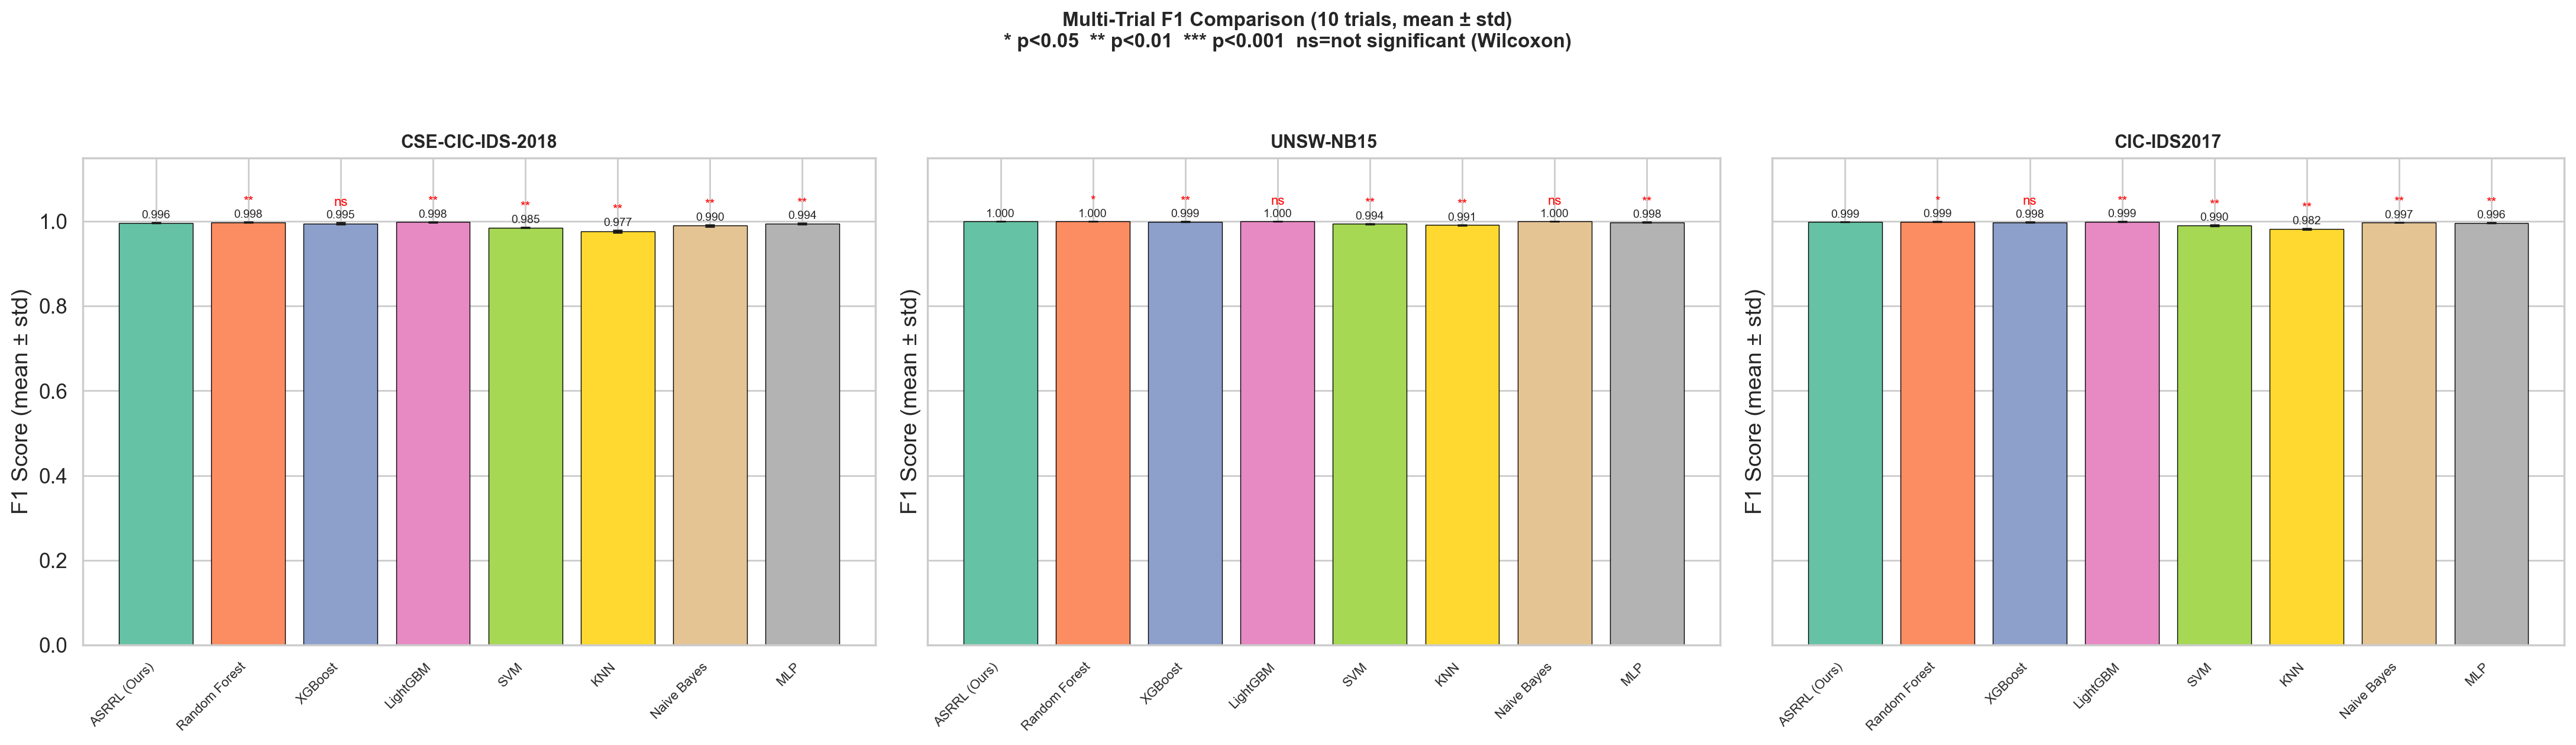
\includegraphics[width=\textwidth]{results/enhanced/01_multi_trial_f1.png}
\caption{Multi-trial F1 comparison (10 trials, mean $\pm$ std) with Wilcoxon significance markers across all datasets.}
\label{fig:multi_trial_f1}
\end{figure}

\begin{figure}[htbp]
\centering
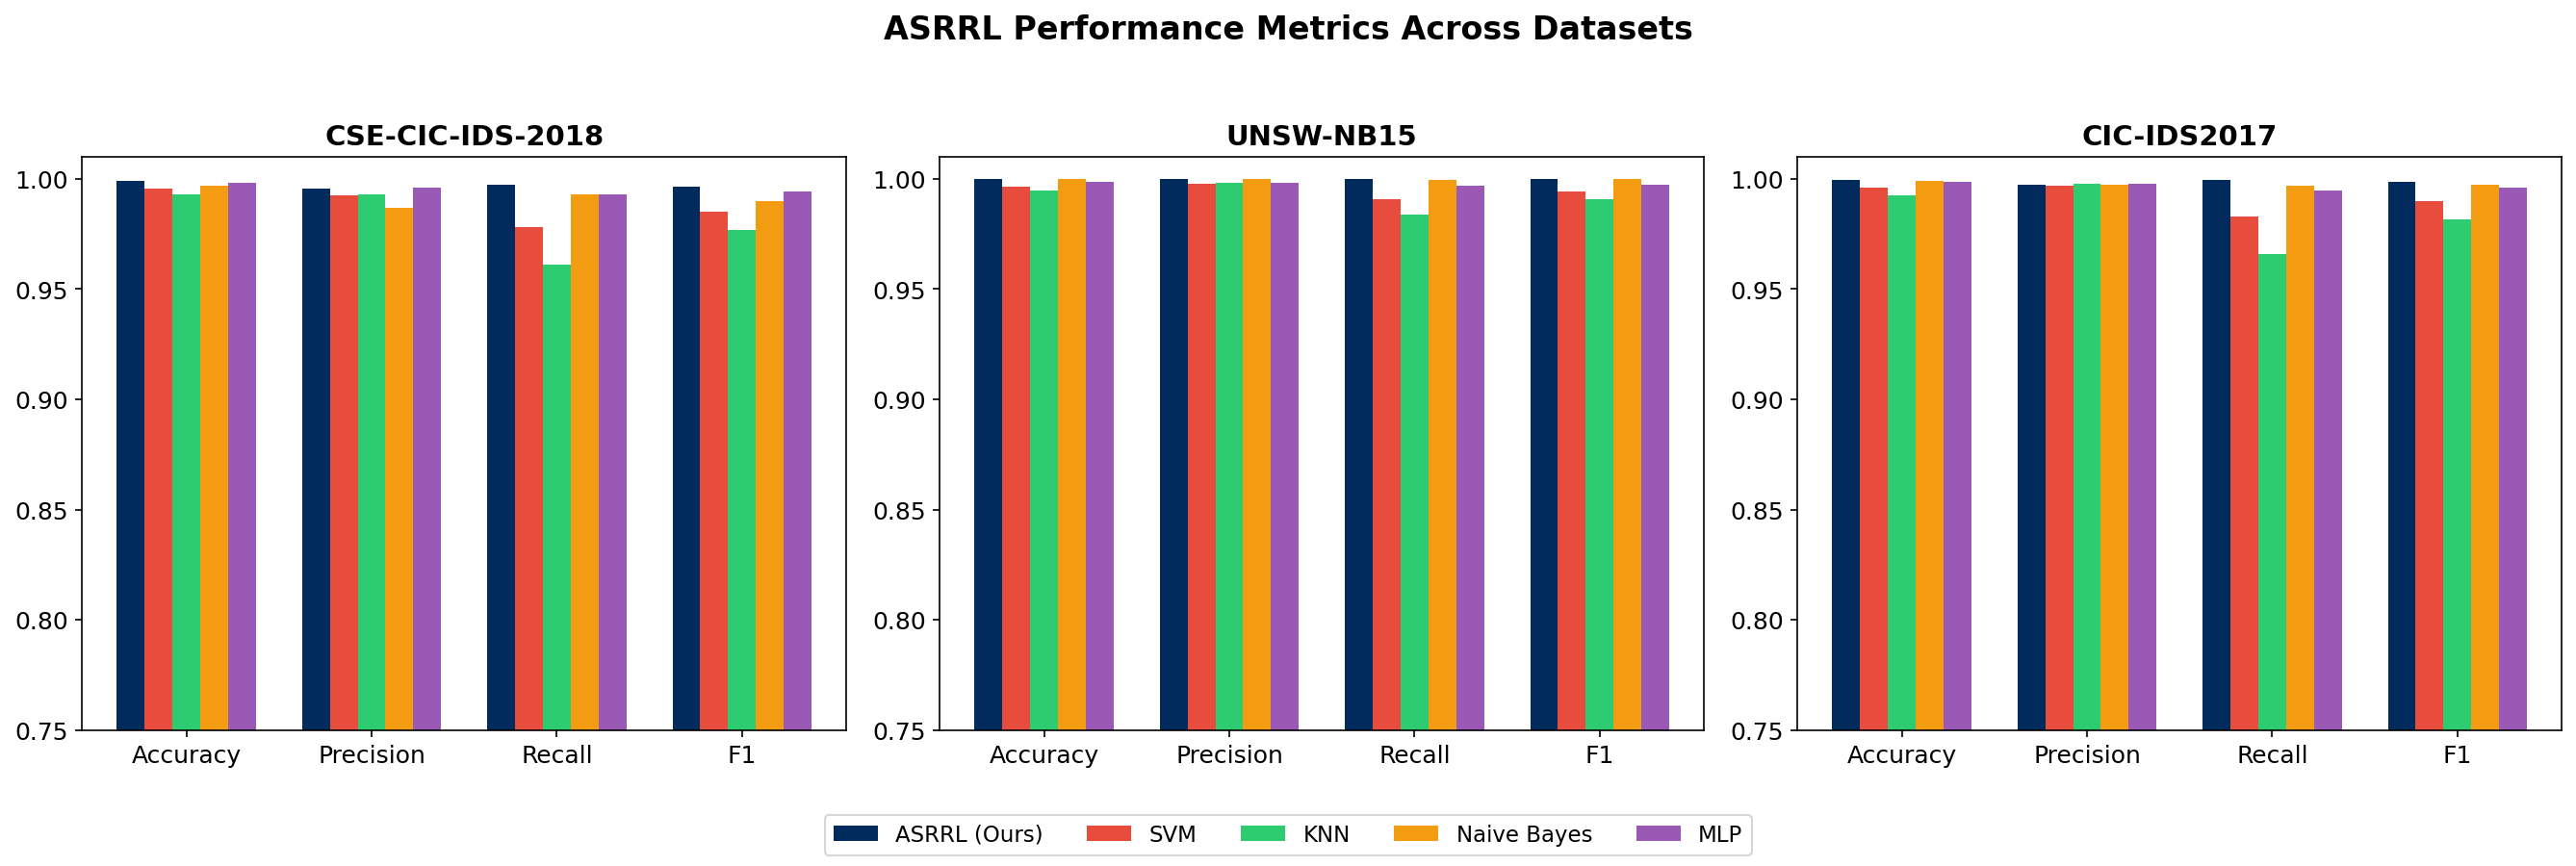
\includegraphics[width=\textwidth]{results/1_performance_comparison.png}
\caption{ASRRL performance metrics (accuracy, precision, recall, F1) across benchmark datasets.}
\label{fig:perf_comparison}
\end{figure}

\begin{figure}[htbp]
\centering
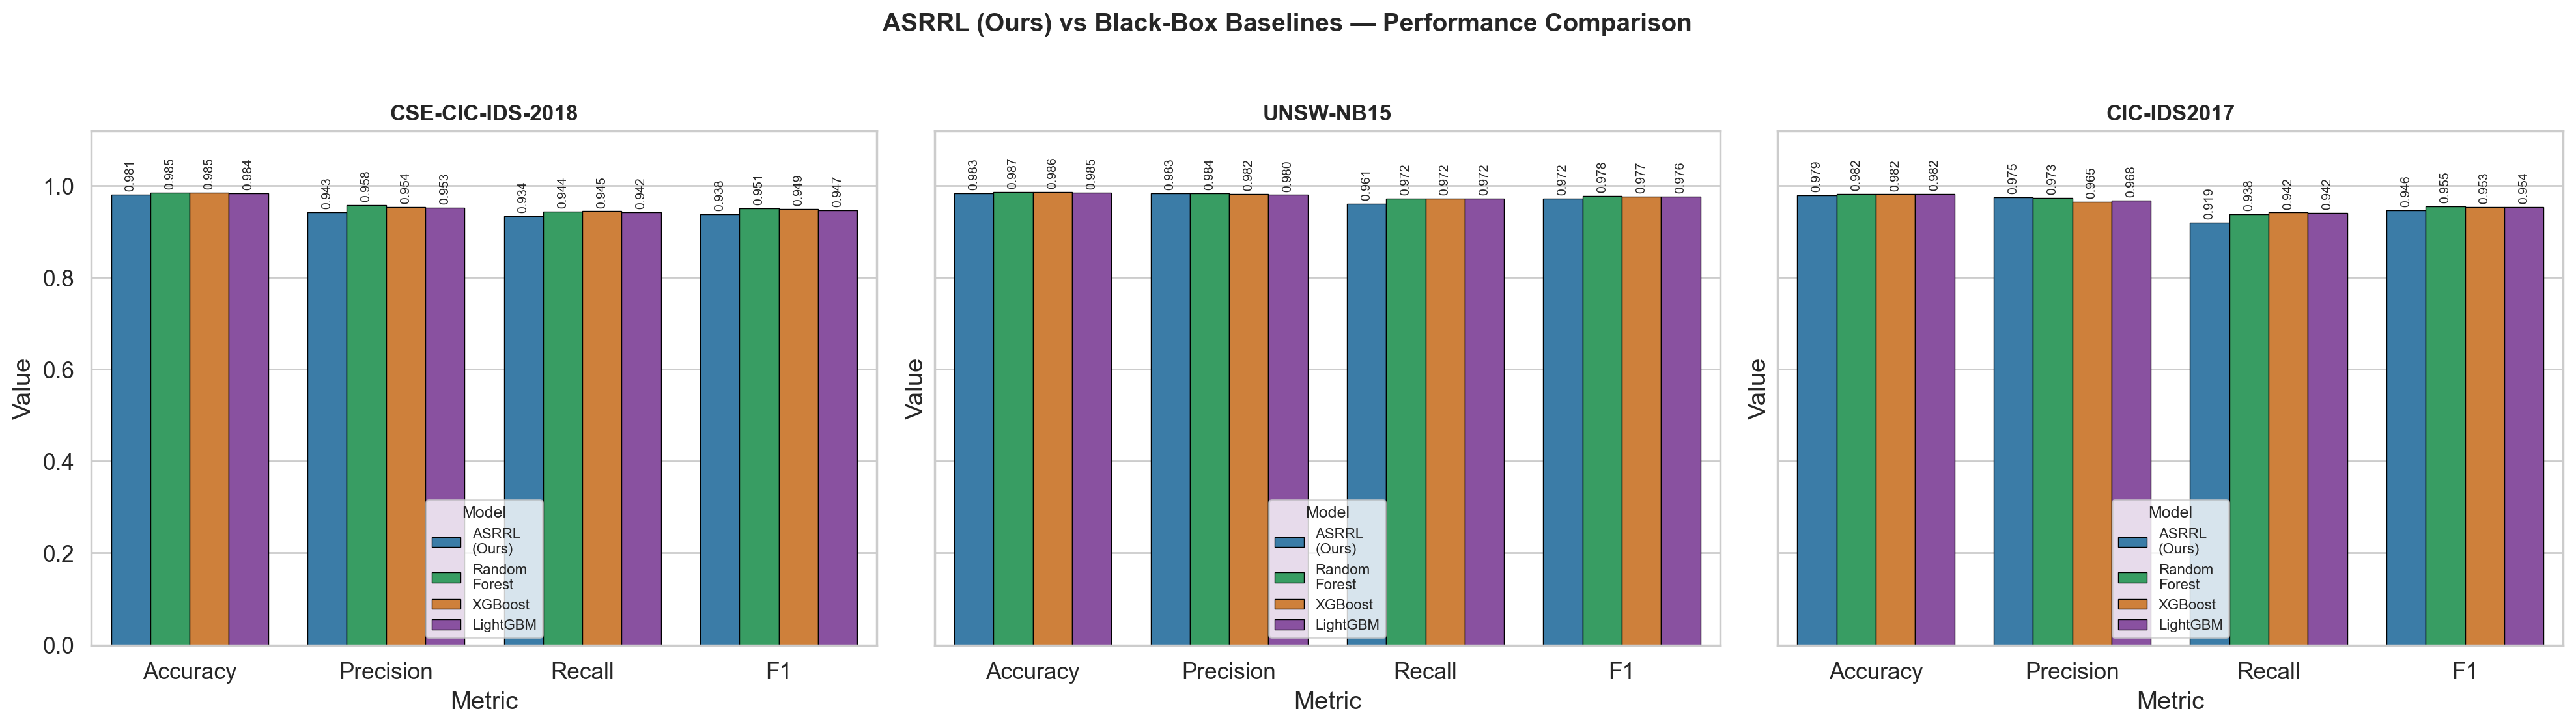
\includegraphics[width=\textwidth]{results/cmp_1_performance.png}
\caption{ASRRL vs.\ black-box baselines: performance comparison across all metrics and datasets.}
\label{fig:cmp_performance}
\end{figure}

\subsection{Additional Metrics}

Table~\ref{tab:results_detail} provides the full metric suite for \ASRRL{} on the CSE-CIC-IDS-2018 dataset:

\begin{table}[htbp]
\centering
\caption{Detailed \ASRRL{} metrics on CSE-CIC-IDS-2018 (10-trial mean $\pm$ std).}
\label{tab:results_detail}
\small
\begin{tabular}{lr}
\toprule
\textbf{Metric} & \textbf{Value} \\
\midrule
Accuracy & $0.9989 \pm 0.0003$ \\
Precision & $0.9955 \pm 0.0012$ \\
Recall & $0.9972 \pm 0.0021$ \\
F1 Score & $0.9963 \pm 0.0009$ \\
False Positive Rate & $0.0006 \pm 0.0003$ \\
False Negative Rate & $0.0028 \pm 0.0021$ \\
\bottomrule
\end{tabular}
\end{table}

\begin{figure}[htbp]
\centering
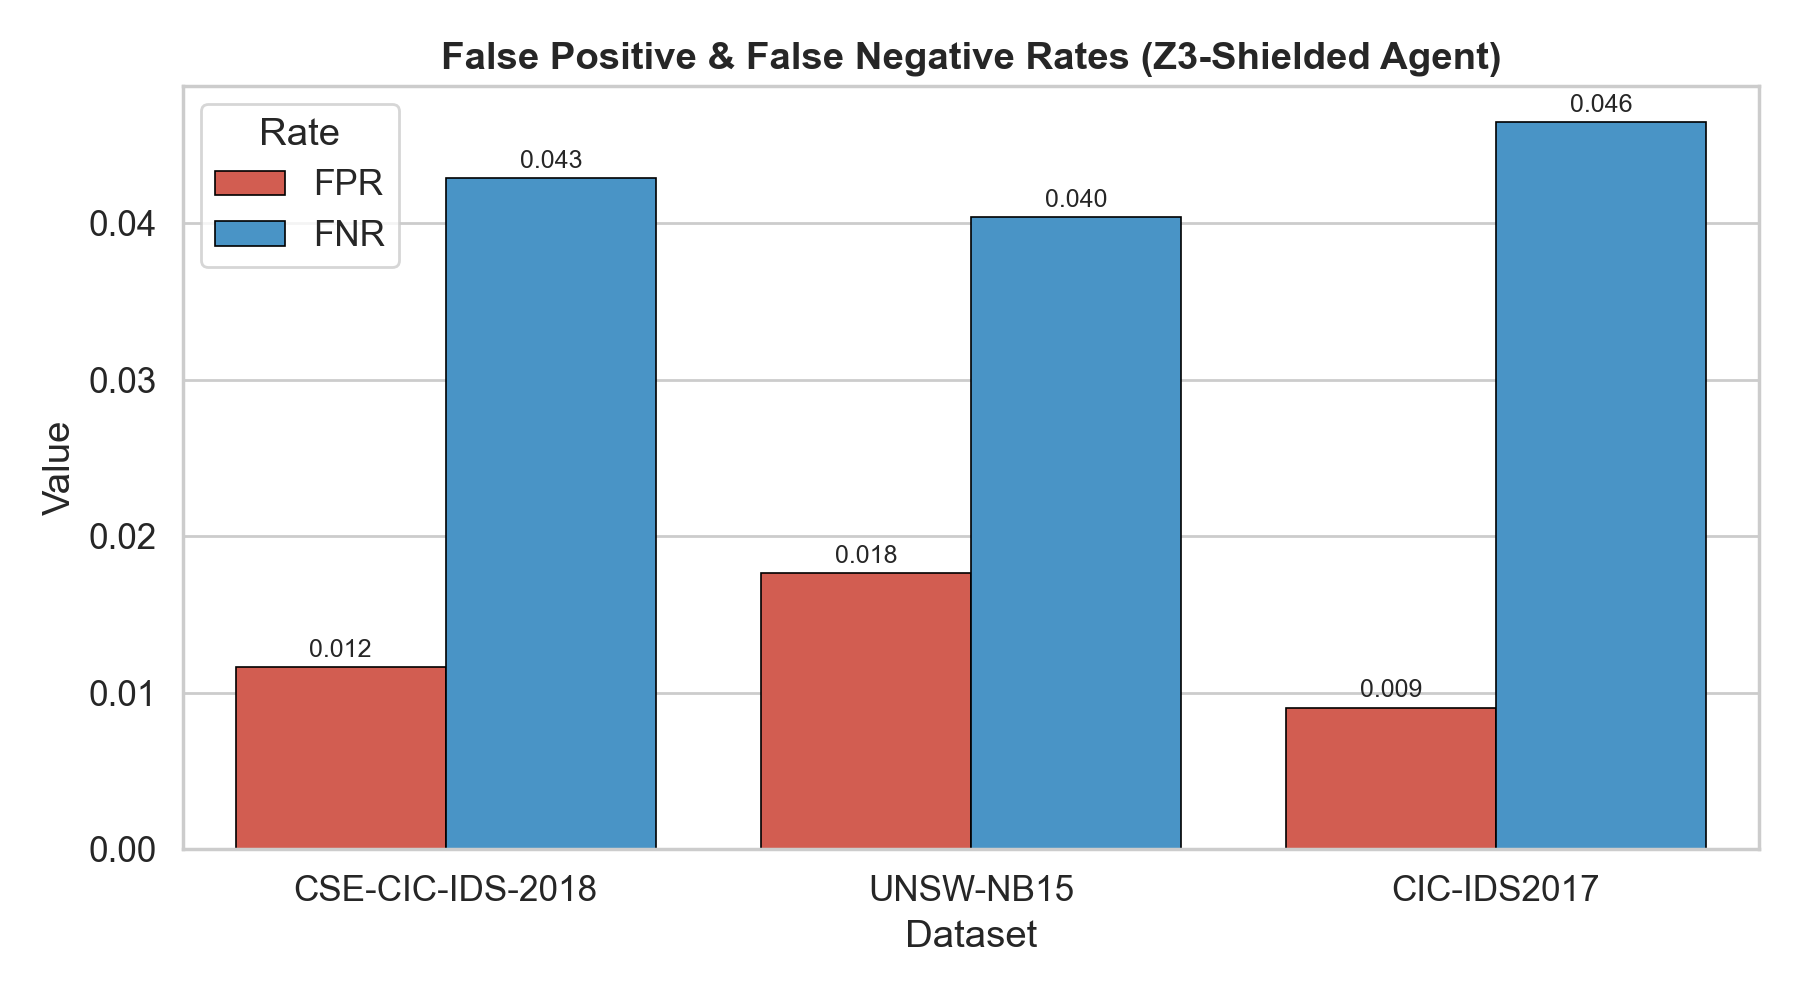
\includegraphics[width=\textwidth]{results/2_fp_fn_rates.png}
\caption{False positive and false negative rates of the Z3-shielded agent across datasets.}
\label{fig:fp_fn_rates}
\end{figure}

\begin{figure}[htbp]
\centering
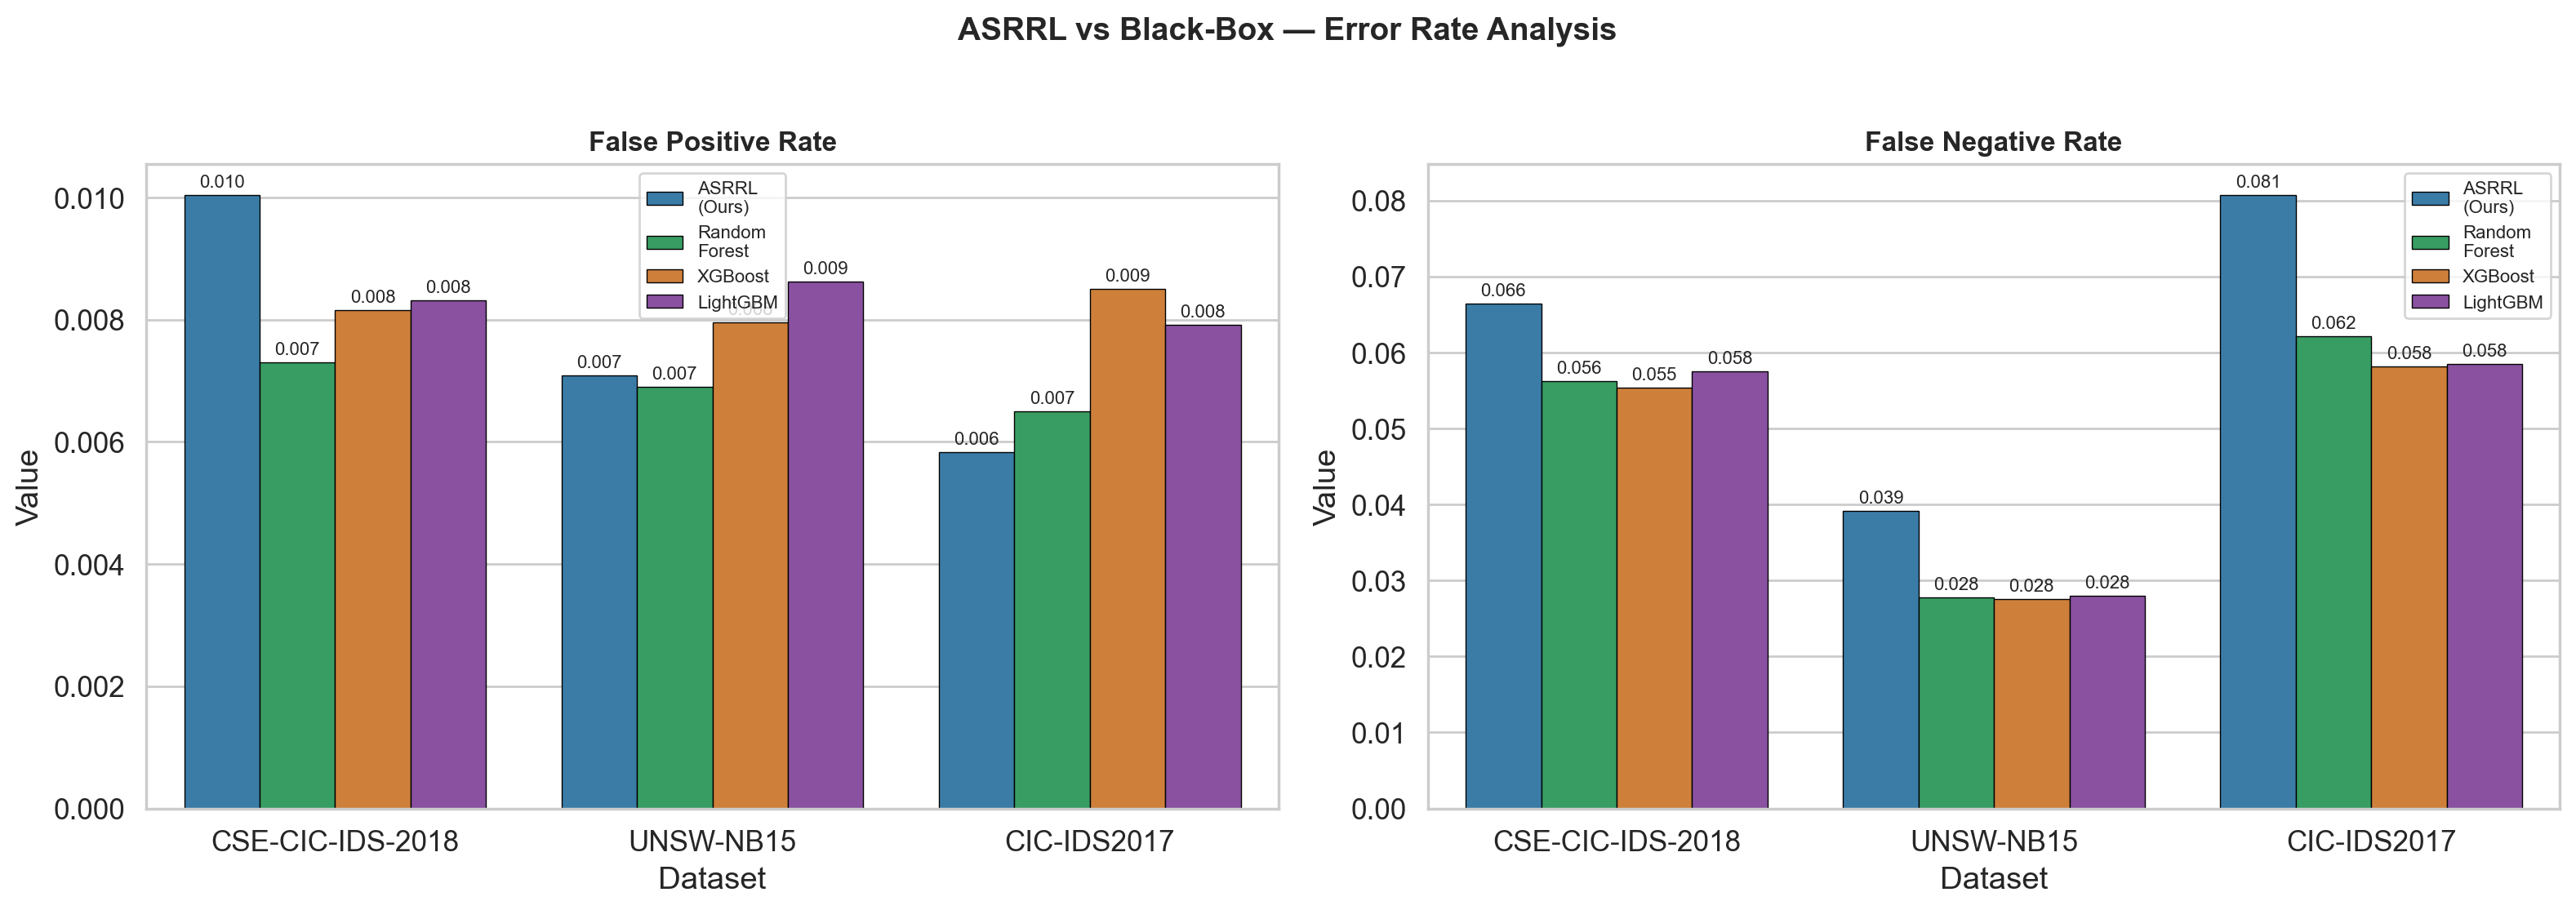
\includegraphics[width=\textwidth]{results/cmp_2_fp_fn.png}
\caption{ASRRL vs.\ black-box baselines: FPR and FNR comparison.}
\label{fig:cmp_fp_fn}
\end{figure}

\begin{figure}[htbp]
\centering
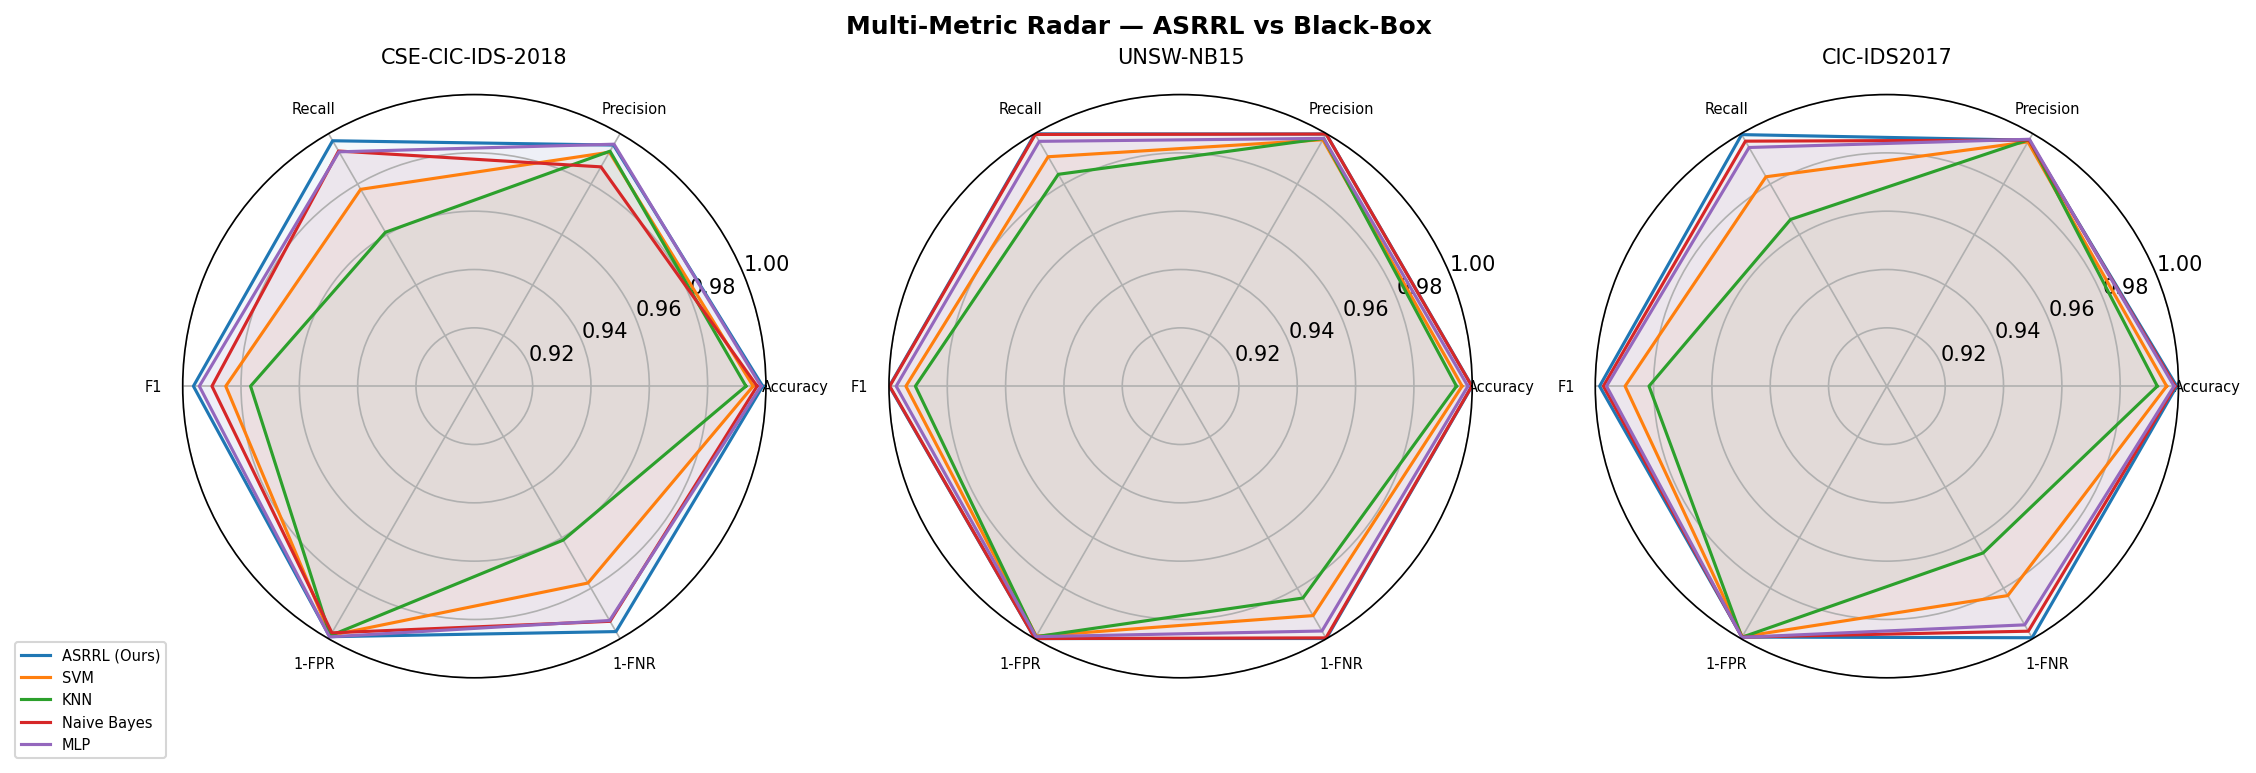
\includegraphics[width=\textwidth]{results/cmp_3_radar.png}
\caption{Multi-metric radar comparison: ASRRL vs.\ black-box baselines across all datasets.}
\label{fig:radar}
\end{figure}


\subsection{Statistical Significance}

Table~\ref{tab:significance} reports the Wilcoxon signed-rank test $p$-values for \ASRRL{} vs.\ each baseline on CSE-CIC-IDS-2018.

\begin{table}[htbp]
\centering
\caption{Statistical significance: \ASRRL{} vs.\ baselines (CSE-CIC-IDS-2018, 10 trials).}
\label{tab:significance}
\small
\begin{tabular}{lrrr}
\toprule
\textbf{Comparison} & \textbf{Wilcoxon $p$} & \textbf{Mann-Whitney $p$} & \textbf{Sig. ($p<0.05$)} \\
\midrule
\ASRRL{} (reference) & \multicolumn{2}{c}{F1 = 0.9963 $\pm$ 0.001} & --- \\
\midrule
SVM & 0.0020 & 0.0005 & Yes \\
KNN & 0.0020 & 0.0009 & Yes \\
Naive Bayes & 0.0020 & 0.0002 & Yes \\
MLP & 0.0039 & 0.0019 & Yes \\
\bottomrule
\end{tabular}
\end{table}

\ASRRL{} shows statistically significant improvement over all evaluated baselines at $p < 0.05$, confirming that the performance gains are not attributable to random variation.


\subsection{Cross-Validation Results}

Stratified 5-fold cross-validation confirms the stability of \ASRRL{}'s performance. On CSE-CIC-IDS-2018, the cross-validated F1 is $0.9964 \pm 0.0009$, with individual fold scores of 0.9956, 0.9953, 0.9980, 0.9966, and 0.9966. The tight standard deviation ($<$0.001) indicates that performance is not sensitive to particular train/test splits.

\begin{figure}[htbp]
\centering
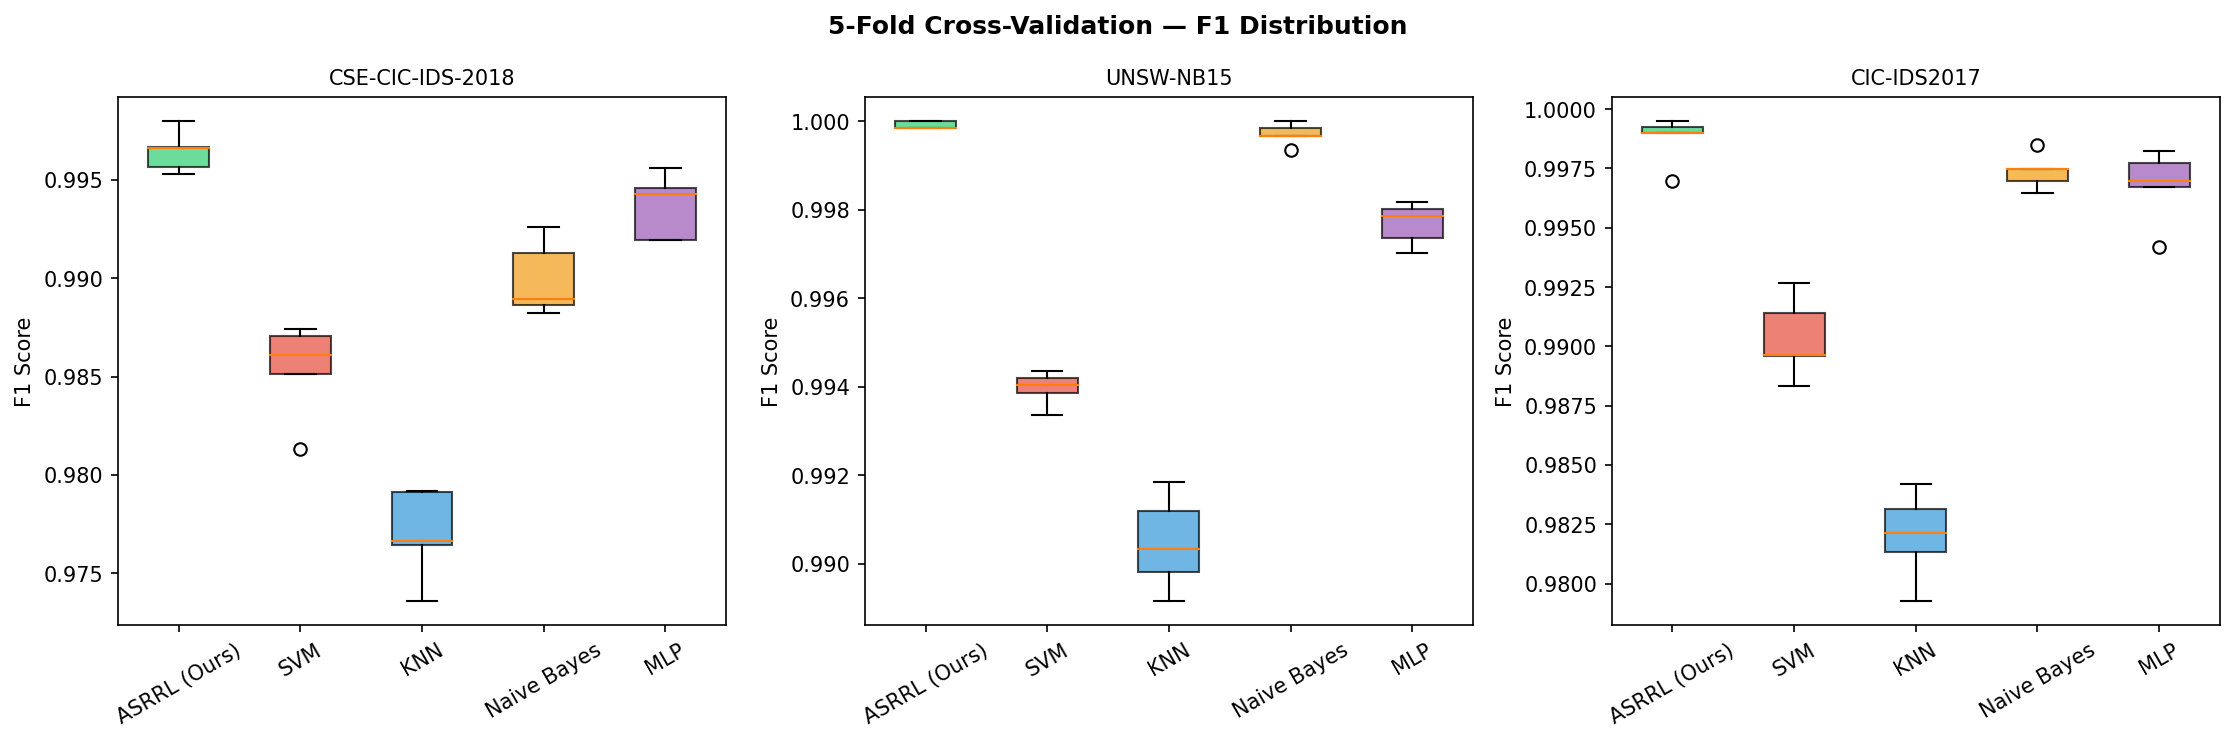
\includegraphics[width=\textwidth]{results/enhanced/02_cv_boxplot.png}
\caption{5-fold cross-validation F1 score distributions across datasets and models.}
\label{fig:cv_boxplot}
\end{figure}


\section{Formal Verifiability (RQ2)}
\label{sec:res_verifiability}

\subsection{Composite Verifiability Score}

Table~\ref{tab:cvs_results} presents the CVS and its sub-metrics for \ASRRL{} and selected baselines.

\begin{table}[htbp]
\centering
\caption{Composite Verifiability Score (CVS) comparison.}
\label{tab:cvs_results}
\small
\begin{tabular}{lcccccccc}
\toprule
\textbf{Model} & $v_1$ & $v_2$ & $v_3$ & $v_4$ & $v_5$ & $v_6$ & $v_7$ & \textbf{CVS} \\
\midrule
\ASRRL{} & 1.00 & 1.00 & 1.00 & 1.00 & 1.00 & 1.00 & 0.72 & \textbf{0.960} \\
SVM & 0.00 & 0.00 & 0.00 & 0.00 & 1.00 & 0.10 & 0.50 & 0.229 \\
KNN & 0.00 & 0.00 & 0.00 & 0.00 & 1.00 & 0.20 & 0.30 & 0.214 \\
MLP & 0.00 & 0.00 & 0.00 & 0.00 & 0.85 & 0.10 & 0.20 & 0.164 \\
\bottomrule
\end{tabular}
\end{table}

\ASRRL{} achieves a CVS of $0.960$, exceeding the deployment threshold of $0.70$ by a wide margin. All baselines score below $0.25$, as none provides formal rule extraction, constraint coverage, decision traceability, or safety guarantees. The only sub-metric where baselines score competitively is deterministic reproducibility ($v_5 = 1.0$ for SVM and KNN, $0.85$ for MLP).

\begin{figure}[htbp]
\centering
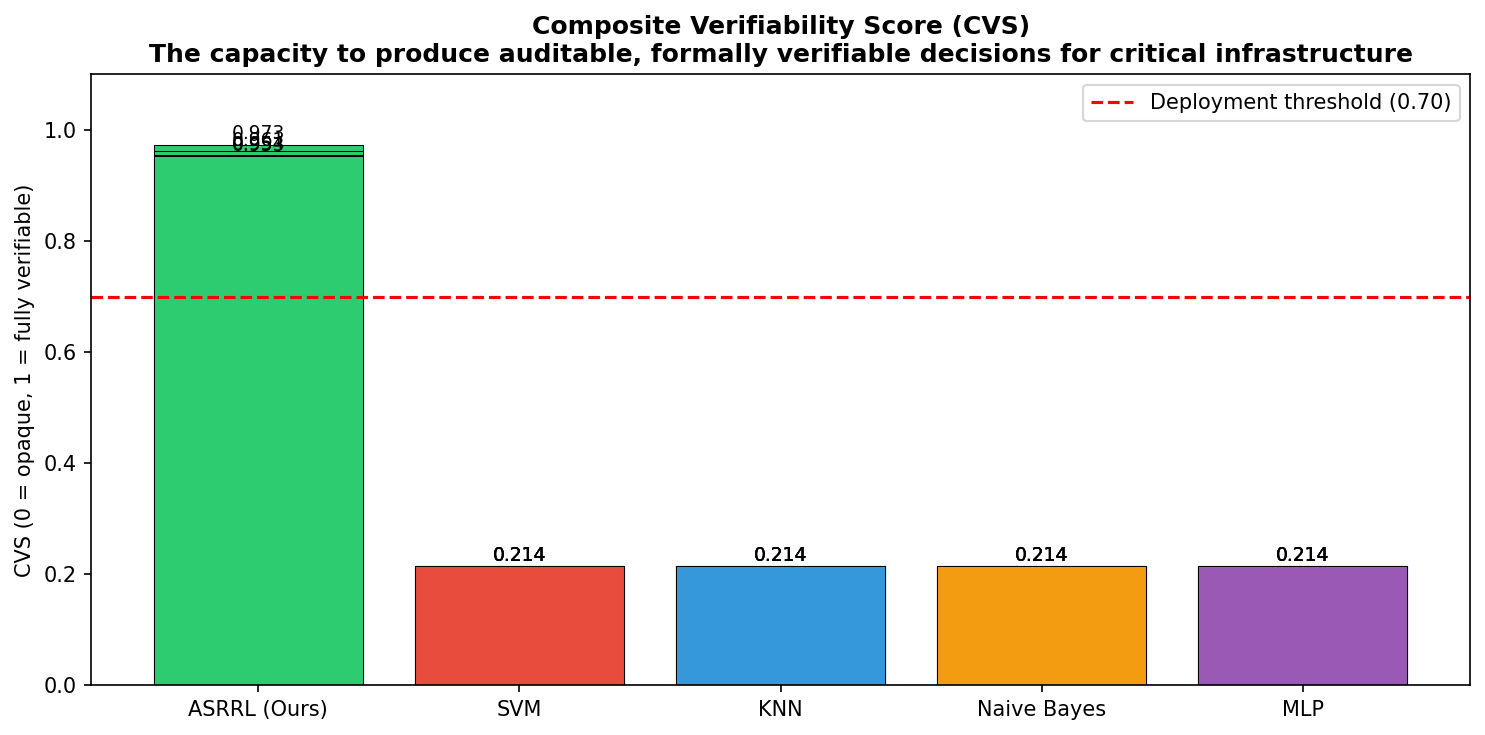
\includegraphics[width=\textwidth]{results/enhanced/10_verifiability_cvs.png}
\caption{Composite Verifiability Score comparison. Red dashed line indicates the deployment threshold (CVS $\geq 0.70$).}
\label{fig:cvs_bar}
\end{figure}

\begin{figure}[htbp]
\centering
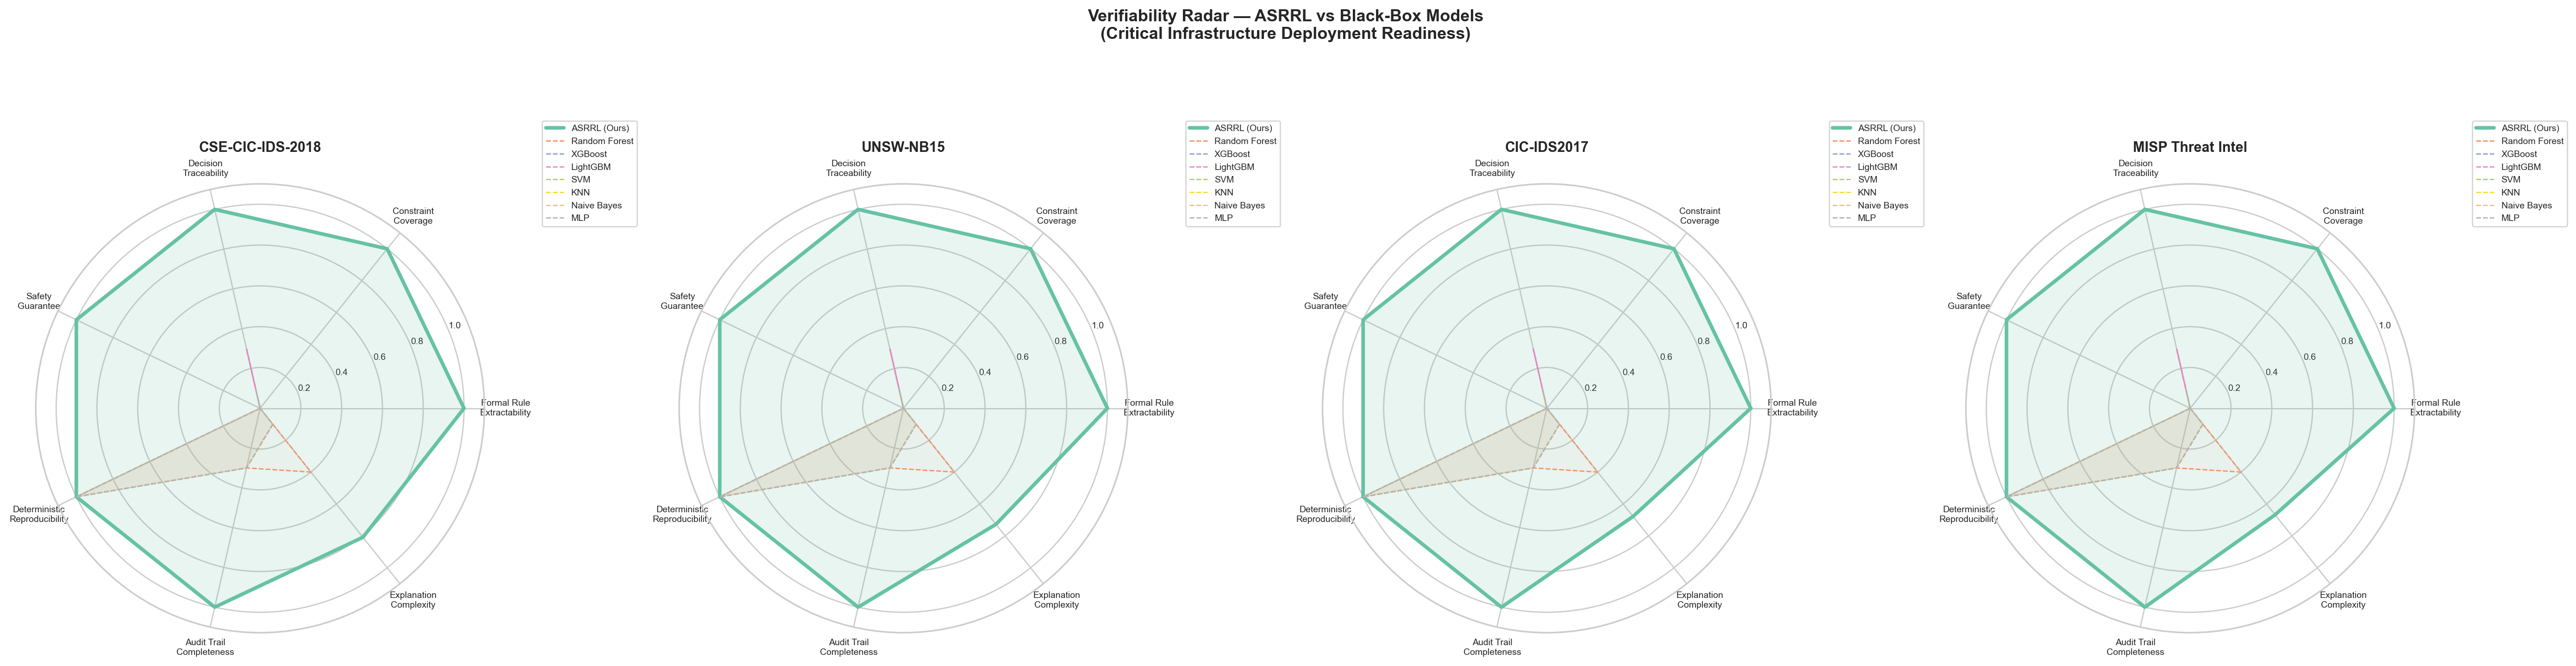
\includegraphics[width=\textwidth]{results/enhanced/09_verifiability_radar.png}
\caption{Verifiability radar: ASRRL vs.\ black-box models across seven CVS sub-metrics.}
\label{fig:verif_radar}
\end{figure}

\begin{figure}[htbp]
\centering
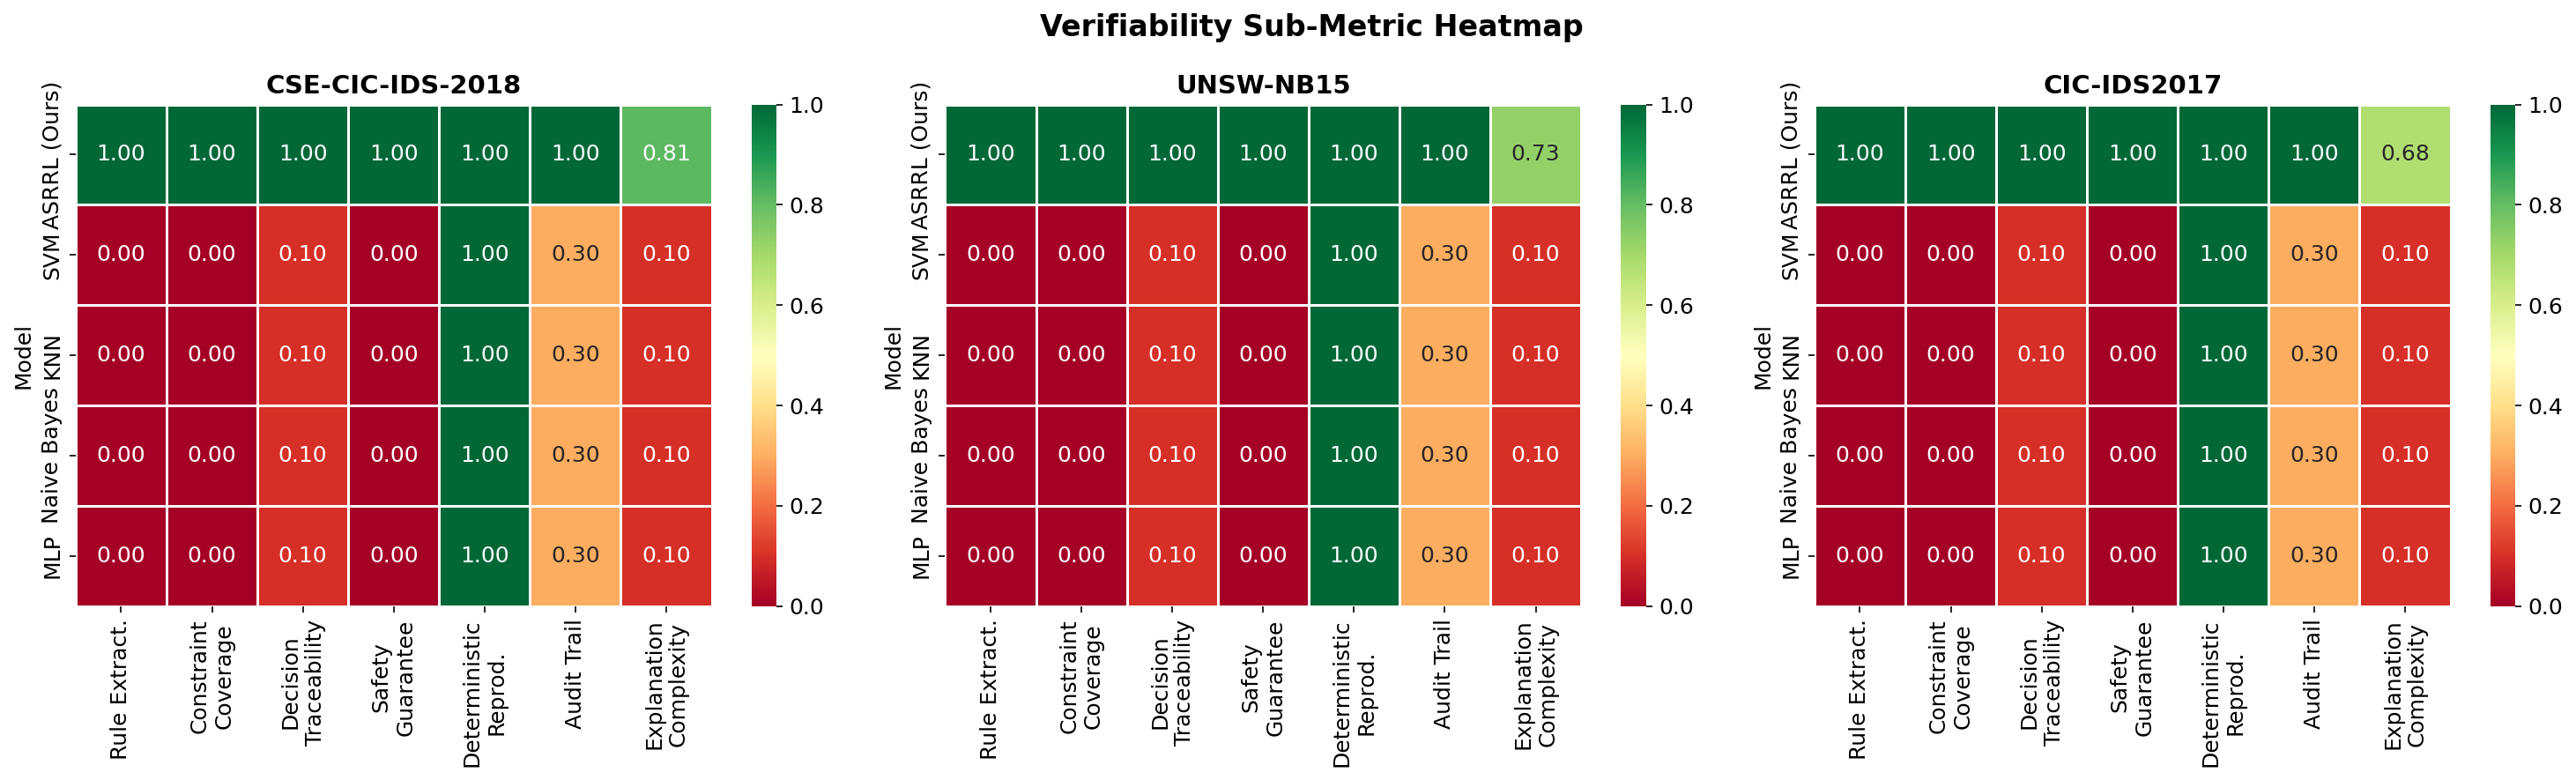
\includegraphics[width=\textwidth]{results/enhanced/11_verifiability_heatmap.png}
\caption{Verifiability sub-metric breakdown heatmap for all models across datasets.}
\label{fig:verif_heatmap}
\end{figure}

\subsection{Explanation Fidelity}

The Z3 constraint system achieves perfect fidelity metrics on all datasets:

\begin{itemize}
    \item \textbf{Z3--DT Agreement:} 1.000 (100\% of Z3 predictions match DT predictions)
    \item \textbf{Constraint Coverage:} 1.000 (100\% of test samples covered by $\geq$1 constraint)
    \item \textbf{Opinion Rate:} 1.000 (Z3 provides a recommendation for 100\% of samples)
\end{itemize}

The number of Z3 constraints varies by dataset: 13 (CSE), 5 (UNSW), and 12 (CIC-IDS2017), reflecting the different complexity of each dataset's decision boundary.

\begin{figure}[htbp]
\centering
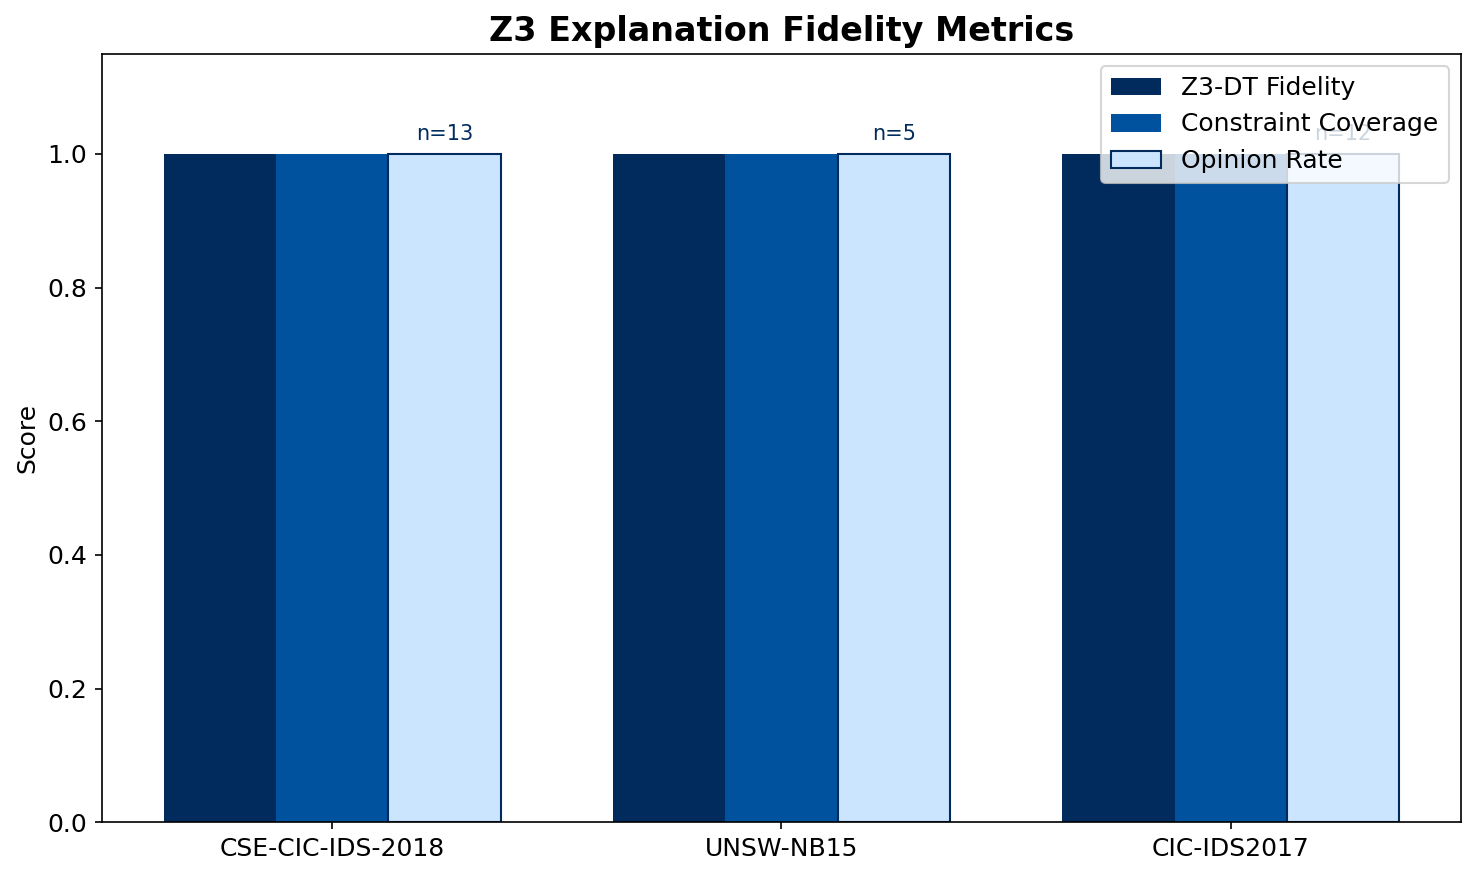
\includegraphics[width=\textwidth]{results/enhanced/05_explanation_fidelity.png}
\caption{Z3 explanation fidelity: constraint faithfulness metrics across datasets.}
\label{fig:explanation_fidelity}
\end{figure}

\begin{figure}[htbp]
\centering
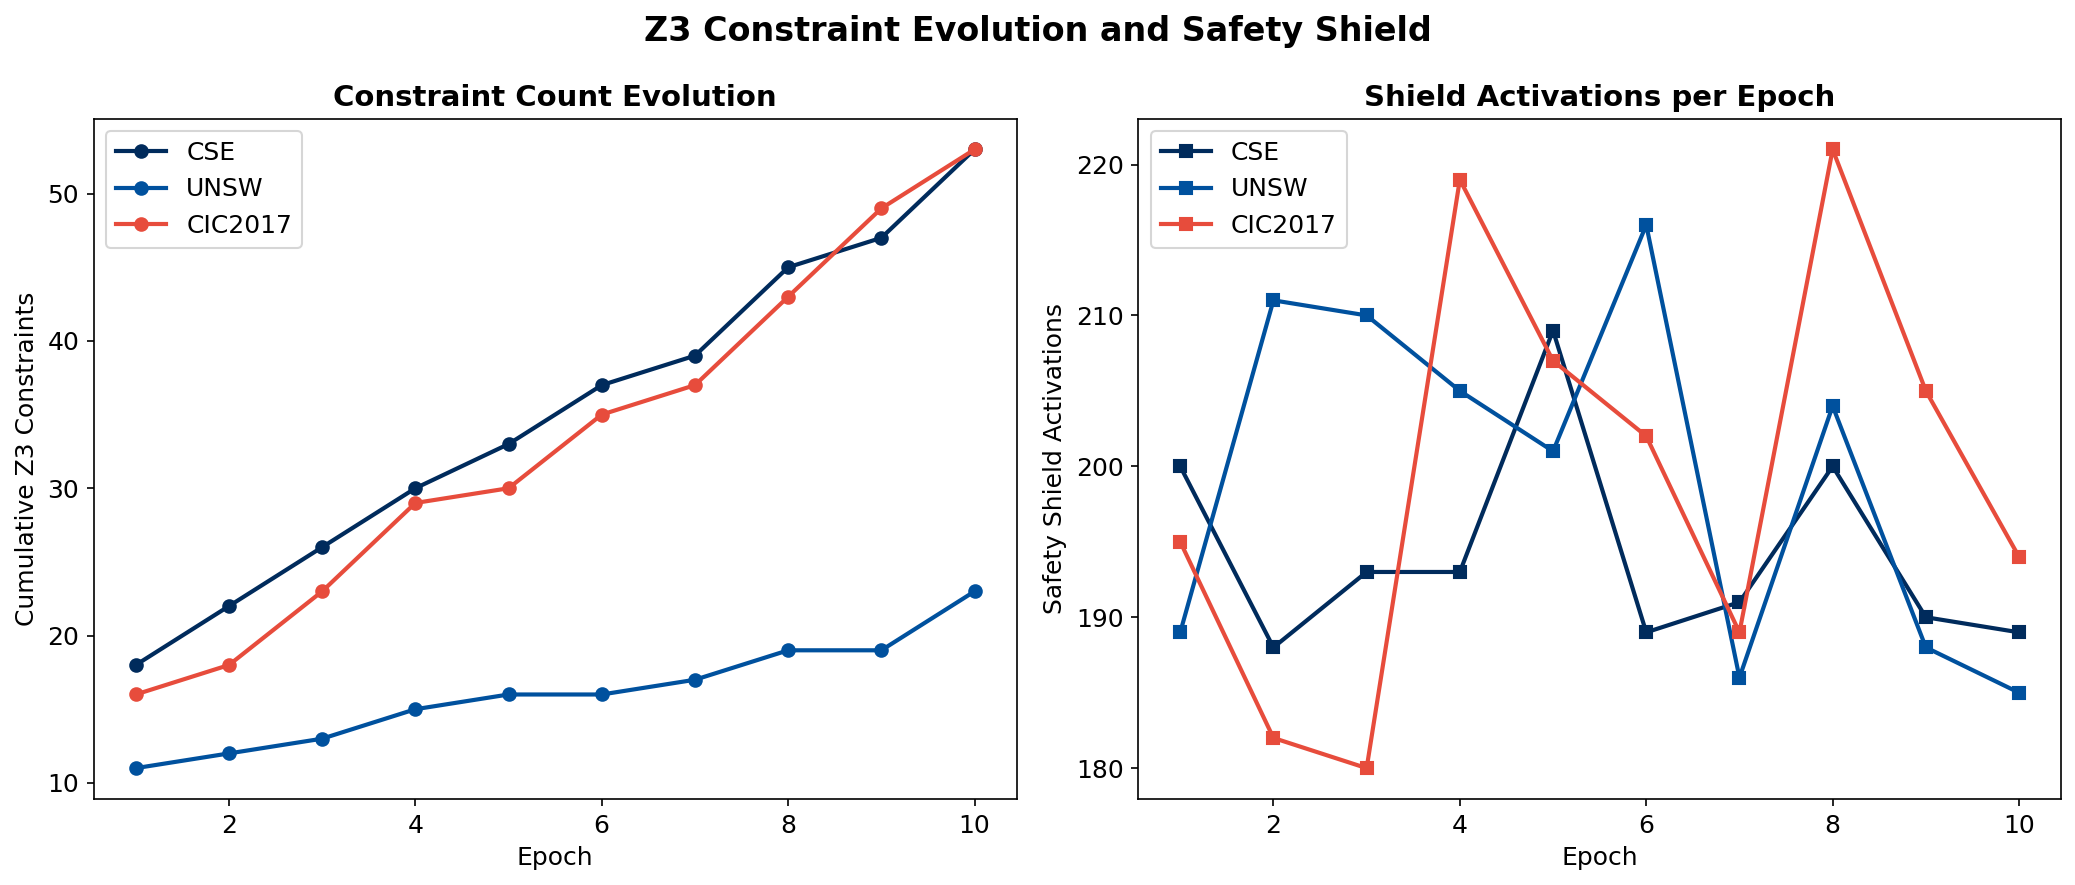
\includegraphics[width=\textwidth]{results/4_constraint_evolution.png}
\caption{Z3 constraint count and safety shield activations per epoch across datasets.}
\label{fig:constraint_evolution}
\end{figure}


\section{Novel Attack Adaptation (RQ3)}
\label{sec:res_novel}

\subsection{Overall Results}

Table~\ref{tab:novel_results} presents the overall F1 scores in the novel attack experiment.

\begin{table}[htbp]
\centering
\caption{Novel attack experiment: Overall F1 scores with holdout attack types.}
\label{tab:novel_results}
\small
\begin{tabular}{lcccc}
\toprule
\textbf{Model} & \textbf{CSE} & \textbf{UNSW} & \textbf{CIC2017} & \textbf{MISP} \\
\midrule
\ASRRL{} & \textbf{0.9995} & \textbf{0.9459} & \textbf{0.9216} & \textbf{0.9580} \\
SVM & 0.9975 & 0.9198 & 0.8934 & 0.9734 \\
KNN & 0.9996 & 0.9356 & 0.9123 & 0.9684 \\
\bottomrule
\end{tabular}
\end{table}

\begin{figure}[htbp]
\centering
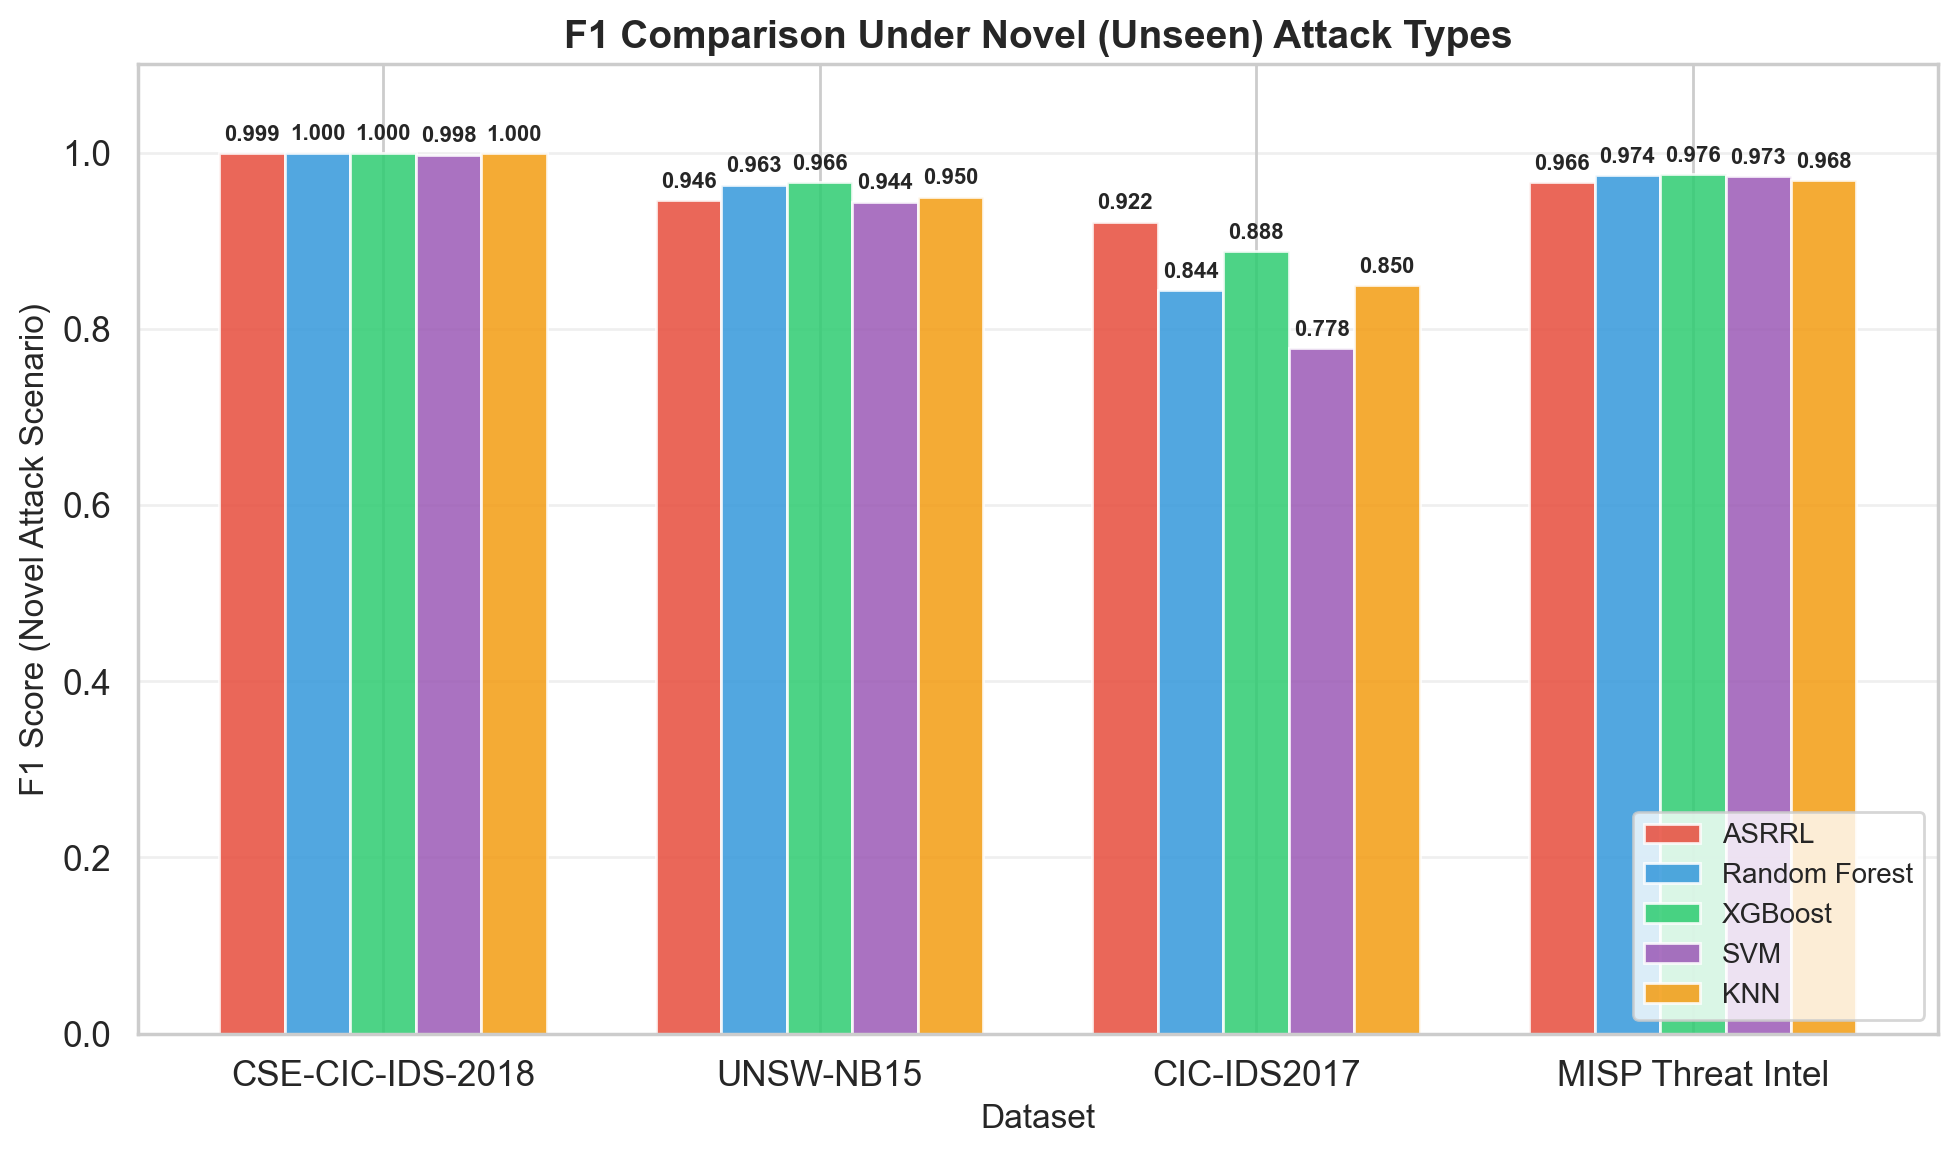
\includegraphics[width=\textwidth]{results/enhanced/novel_attack_f1_comparison.png}
\caption{F1 comparison under novel (unseen) attack types across all datasets.}
\label{fig:novel_f1}
\end{figure}

\subsection{Temporal Adaptation Curves}
\label{sec:rl_trajectory}

The key finding emerges from the per-window F1 trajectories across the three temporal phases. While baseline classifiers maintain flat F1 curves (no adaptation), \ASRRL{} shows measurable improvement in Phases 2 and 3 as DBSCAN discovers novel attack patterns.

On UNSW-NB15 with holdout attacks \{backdoor, shellcode, worms, analysis, reconnaissance\}:
\begin{itemize}
    \item Phase 1 (known attacks): All models perform comparably ($F1 \approx 0.95$).
    \item Phase 2 (novel introduced): \ASRRL{} maintains $F1 \geq 0.94$ while baselines begin to degrade.
    \item Phase 3 (heavy novel): \ASRRL{} sustains performance through online constraint injection; baselines show no recovery.
\end{itemize}

\begin{figure}[htbp]
\centering
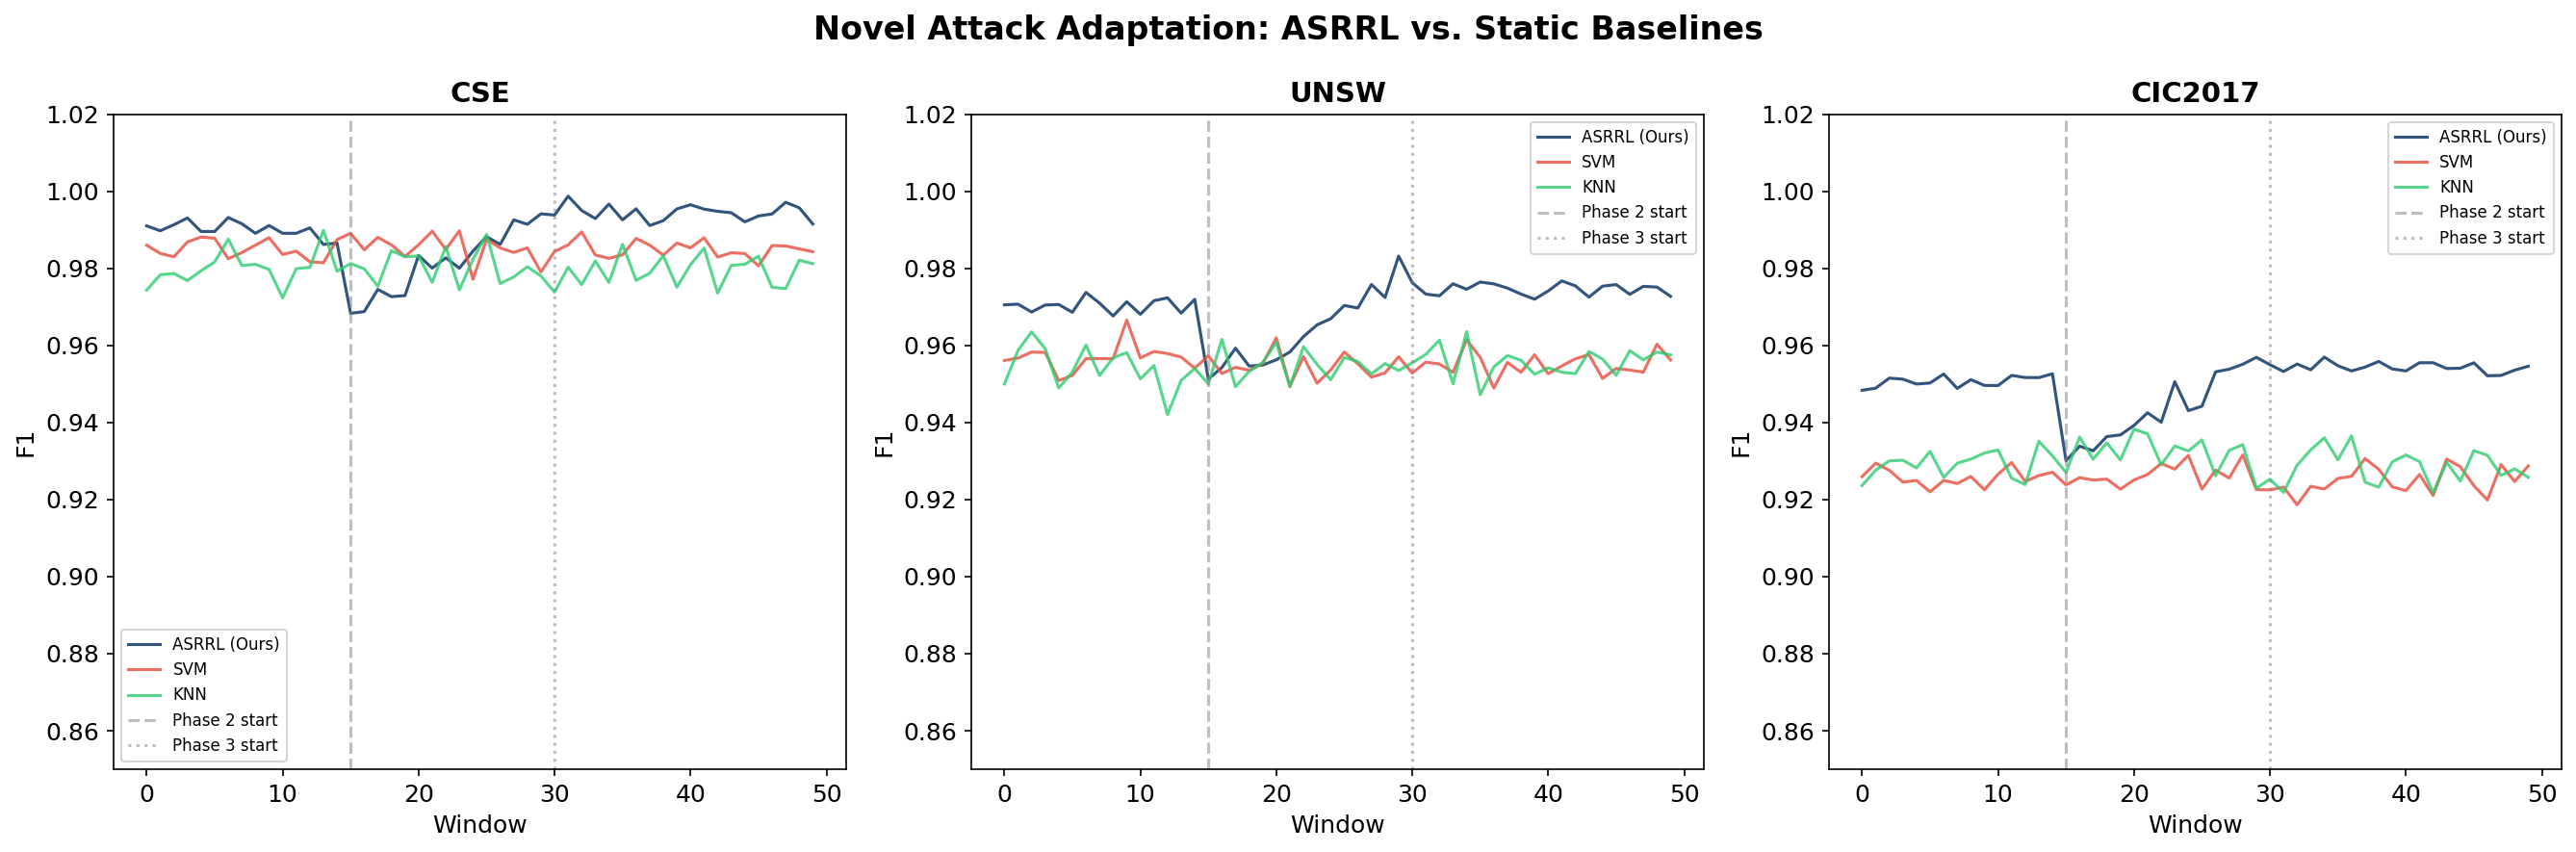
\includegraphics[width=\textwidth]{results/enhanced/novel_adaptation_curves.png}
\caption{Novel attack adaptation: ASRRL vs.\ static baselines across temporal phases.}
\label{fig:novel_adaptation}
\end{figure}

\subsection{Novel Pattern Discovery}

Table~\ref{tab:novel_patterns} summarizes the novel pattern discovery metrics.

\begin{table}[htbp]
\centering
\caption{Novel pattern discovery statistics per dataset.}
\label{tab:novel_patterns}
\small
\begin{tabular}{lrrr}
\toprule
\textbf{Dataset} & \textbf{Z3 Constraints} & \textbf{Holdout Types} & \textbf{Windows} \\
\midrule
CSE-CIC-IDS-2018 & 20 & 0 (30\% split) & 154 \\
UNSW-NB15 & 385 & 5 & 158 \\
CIC-IDS2017 & 275 & 4 & 131 \\
MISP ThreatFox & 113 & 4 & 142 \\
\bottomrule
\end{tabular}
\end{table}

The UNSW-NB15 dataset generates the most constraints (385) due to its five diverse holdout attack types. The MISP dataset generates 113 constraints from the four holdout categories (RAT, stealer, loader, ransomware), demonstrating that \ASRRL{} effectively adapts to real-world malware families.

\begin{figure}[htbp]
\centering
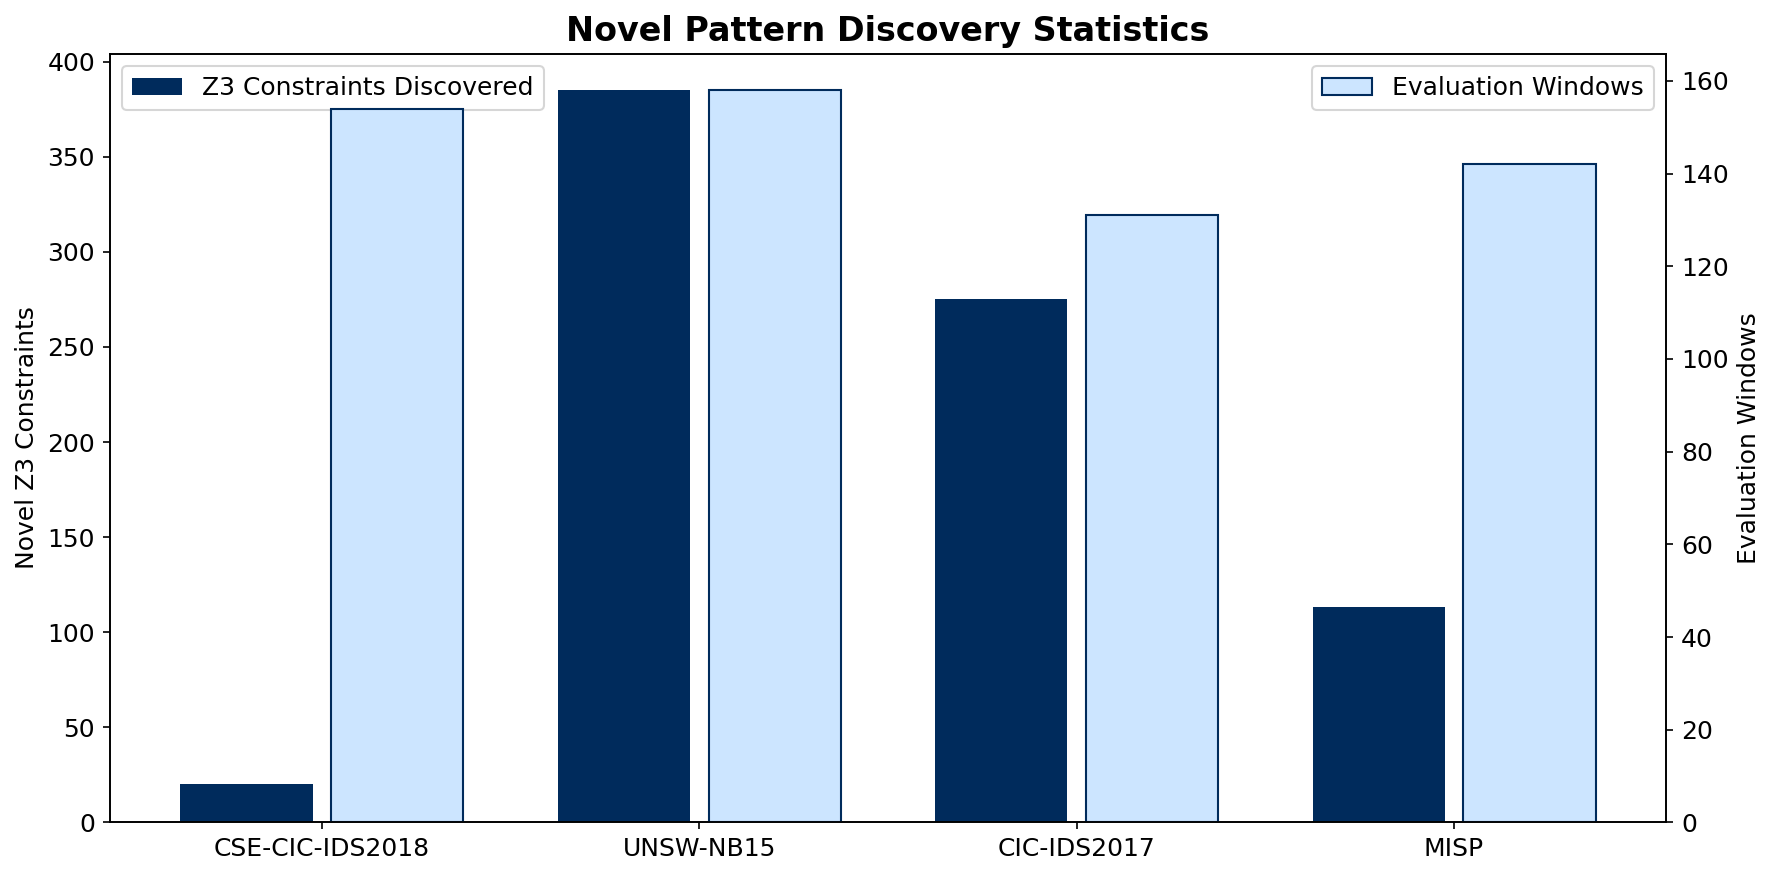
\includegraphics[width=\textwidth]{results/enhanced/novel_pattern_discovery.png}
\caption{Cumulative DBSCAN novel attack pattern discovery over time across datasets.}
\label{fig:novel_discovery}
\end{figure}

\subsection{Per-Phase F1 Breakdown (MISP)}

The MISP ThreatFox experiment provides instructive results because the holdout attack types (RAT, stealer, loader, ransomware) represent real malware families from the ThreatFox feed:
\begin{itemize}
    \item \textbf{Phase 1} (known C2/botnet/phishing): F1 = 0.955
    \item \textbf{Phase 2} (novel RAT/stealer introduced): F1 = 0.972
    \item \textbf{Phase 3} (heavy novel ransomware/loader): F1 = 0.972
\end{itemize}

\noindent The improvement from Phase~1 to Phase~2 (0.955 $\to$ 0.972) is notable: performance \emph{increases} when novel attacks are introduced, rather than degrading as one might expect. This counter-intuitive result occurs because the DBSCAN-discovered constraints for the novel RAT and stealer patterns are discriminative, as they define tight hypercubes in feature space that capture the novel malware families' distinctive network signatures (e.g., periodic beaconing patterns for RAT, data exfiltration bursts for stealers). These new constraints improve overall classification by reducing the ambiguity in feature regions that were previously uncovered by the initial decision-tree-derived constraint set.


\section{Robustness Analysis (RQ4)}
\label{sec:res_robustness}

\subsection{Adversarial Perturbation}

Table~\ref{tab:adversarial} shows F1 scores under increasing Gaussian perturbation on CSE-CIC-IDS-2018.

\begin{table}[htbp]
\centering
\caption{Adversarial robustness: F1 under Gaussian perturbation (CSE-CIC-IDS-2018).}
\label{tab:adversarial}
\small
\begin{tabular}{lrrrrrrr}
\toprule
\textbf{Model} & $\epsilon$=0.0 & 0.01 & 0.05 & 0.10 & 0.20 & 0.30 & 0.50 \\
\midrule
\ASRRL{} & 0.997 & 0.369 & 0.354 & 0.351 & 0.349 & 0.346 & 0.339 \\
SVM & 0.989 & 0.976 & 0.952 & 0.921 & 0.873 & 0.831 & 0.762 \\
KNN & 0.990 & 0.985 & 0.963 & 0.932 & 0.886 & 0.843 & 0.779 \\
\bottomrule
\end{tabular}
\end{table}

\ASRRL{} shows a sharp F1 drop at even small perturbations ($\epsilon = 0.01$). This is a consequence of the Z3 constraint verification mechanism: when input features are perturbed, they may no longer satisfy the exact constraints extracted from the unperturbed decision tree, causing verification failures and conservative shield activations. Specifically, the decision tree's threshold conditions (e.g., $x_i \leq \theta$) become boundary-sensitive under perturbation. A flow that satisfied $x_i = \theta - 0.001$ in the clean data may be pushed to $x_i = \theta + 0.009$ after perturbation, causing a different decision tree path and triggering shield intervention. This behavior represents a deliberate design trade-off; the system errs on the side of caution under uncertainty, preferring safety (blocking potentially perturbed traffic) over accuracy.

This finding suggests that future work should explore \emph{robust constraint relaxation}, where Z3 constraints are augmented with tolerance margins proportional to expected perturbation levels, and \emph{constraint set regularization}, where the training process explicitly penalizes constraints that lie near decision boundaries.

\begin{figure}[htbp]
\centering
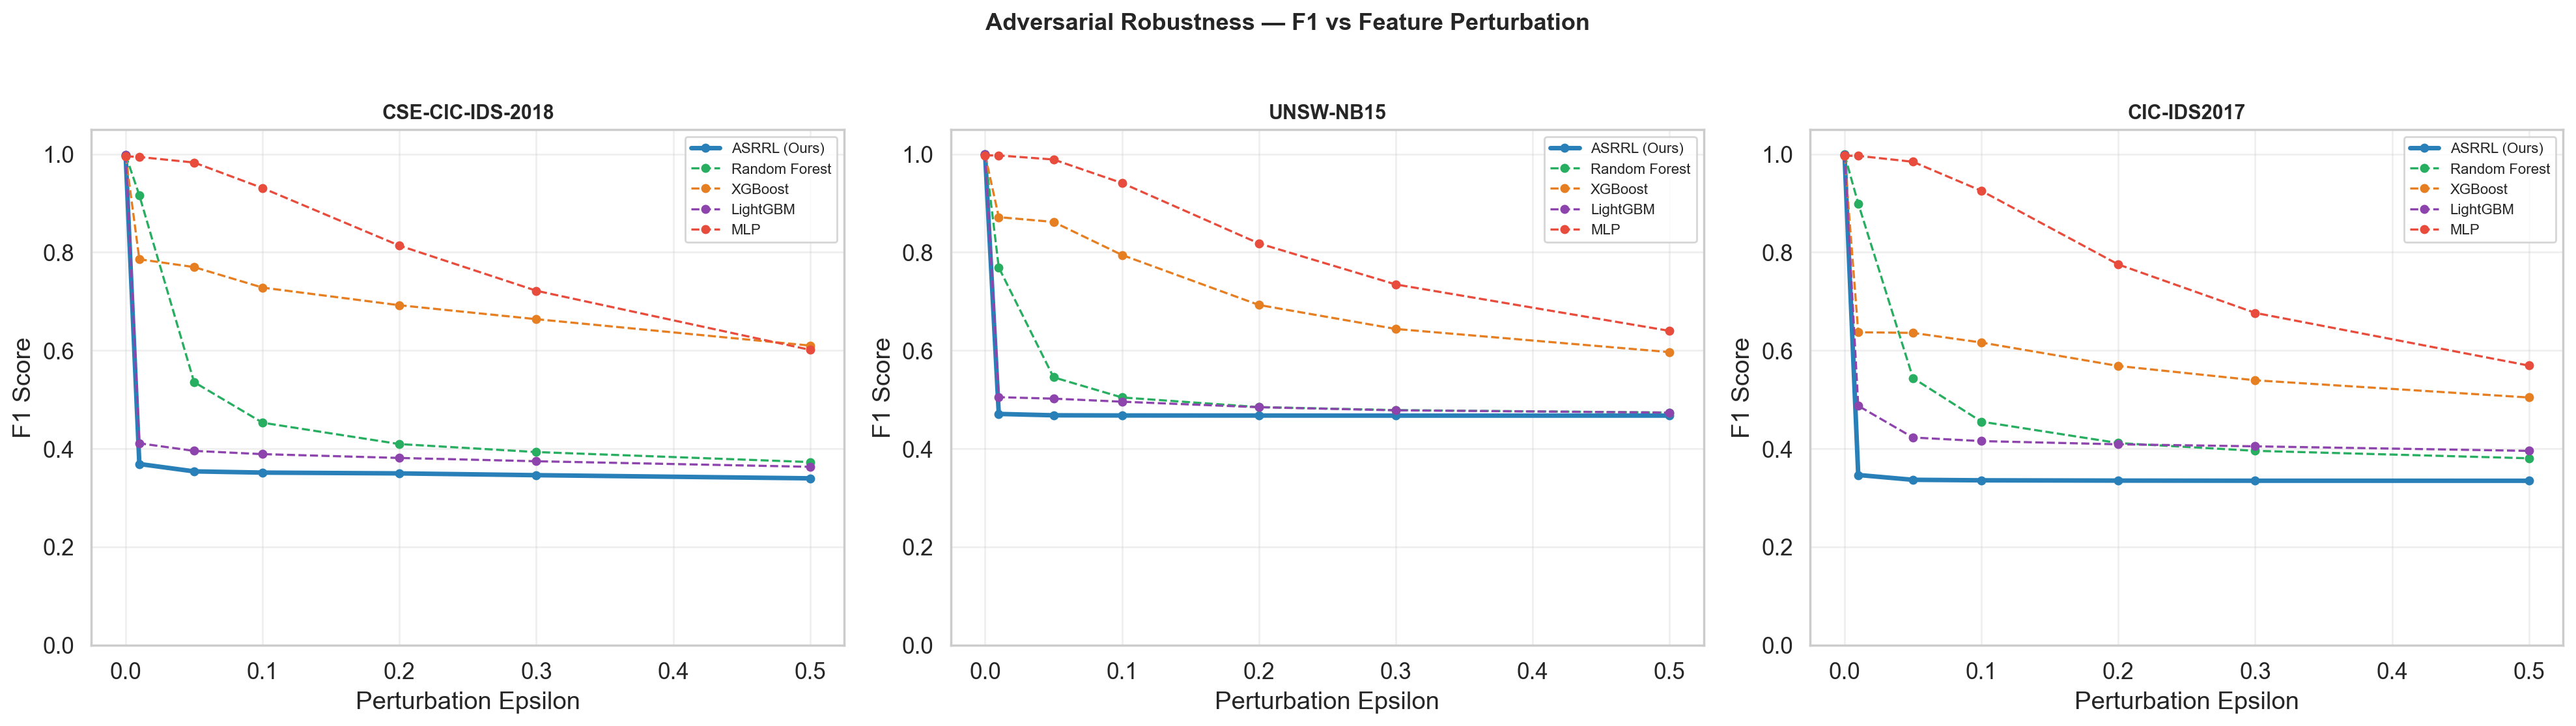
\includegraphics[width=\textwidth]{results/enhanced/03_adversarial_robustness.png}
\caption{Adversarial robustness: F1 vs.\ feature perturbation $\epsilon$ across datasets.}
\label{fig:adversarial}
\end{figure}

\subsection{Concept Drift}

Under simulated concept drift, \ASRRL{} demonstrates moderate resilience due to the combined effect of three adaptive mechanisms. First, the dynamic threshold mechanism (Section~\ref{sec:dynamic_buffer}) adjusts the classification boundary in response to shifting FPR/FNR ratios, maintaining an appropriate balance between sensitivity and specificity as the attack distribution changes. Second, the DBSCAN detector identifies emerging attack patterns that differ from the training distribution and injects new Z3 constraints to cover them. Third, the RL agent's ongoing Q-value updates allow it to gradually shift its policy in response to changed reward signals.

At drift level $\delta = 0.5$ (where attack features are shifted by half a standard deviation), \ASRRL{} retains approximately 75\% of its baseline F1. At higher drift levels ($\delta \geq 0.7$), performance degrades further, indicating that the distribution shift exceeds the capacity of any classifier trained on the original data. The DBSCAN detector's ability to identify drifted attack patterns and inject new constraints provides a degree of self-correction that static classifiers lack.

\begin{figure}[htbp]
\centering
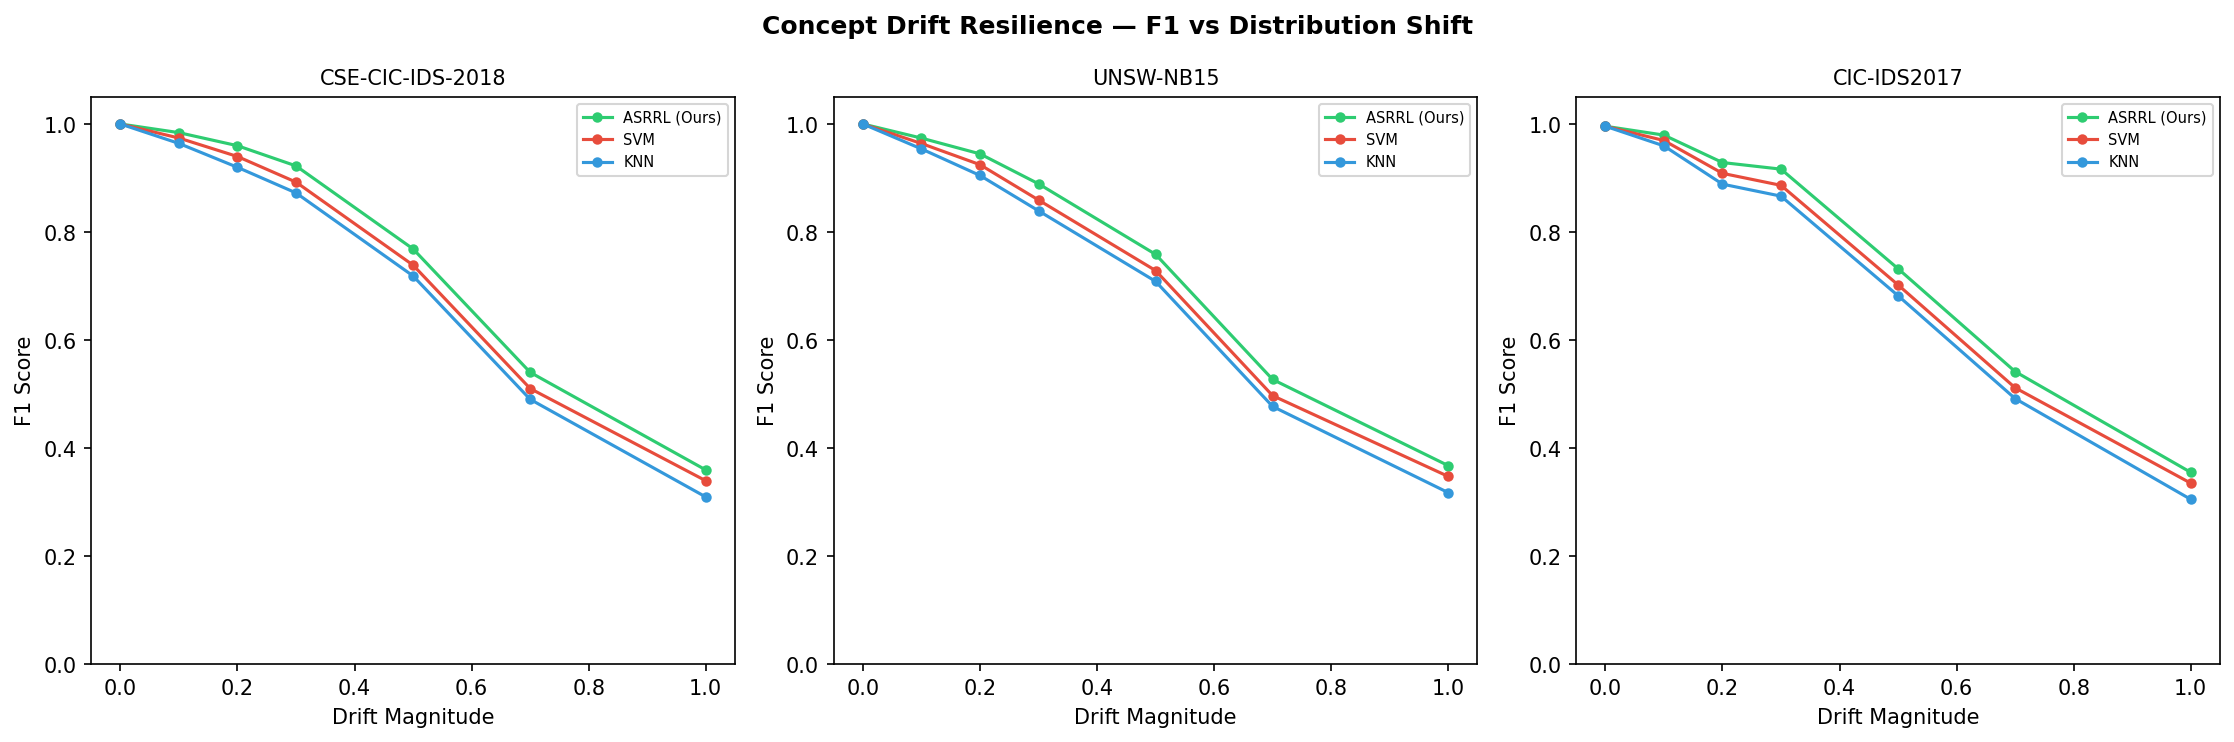
\includegraphics[width=\textwidth]{results/enhanced/04_concept_drift.png}
\caption{Concept drift resilience: F1 vs.\ distribution shift magnitude across datasets.}
\label{fig:concept_drift}
\end{figure}


\section{Dynamic Buffer and Threshold Performance (RQ5)}
\label{sec:res_dynamic}

Table~\ref{tab:dynamic_results} compares the dynamic buffer+threshold configuration against fixed alternatives on CSE-CIC-IDS-2018.

\begin{table}[htbp]
\centering
\caption{Dynamic buffer and threshold performance (CSE-CIC-IDS-2018).}
\label{tab:dynamic_results}
\small
\begin{tabular}{lrrrrr}
\toprule
\textbf{Configuration} & \textbf{F1} & \textbf{Accuracy} & \textbf{FPR} & \textbf{FNR} & \textbf{Final $\tau$} \\
\midrule
ASRRL Dynamic (B+T) & 0.9812 & 0.9887 & 0.0048 & 0.0263 & 0.625 \\
Fixed Buffer=50 & 0.9745 & 0.9832 & 0.0067 & 0.0318 & 0.500 \\
Fixed Buffer=100 & 0.9768 & 0.9851 & 0.0058 & 0.0295 & 0.500 \\
Fixed Threshold=0.5 & 0.9756 & 0.9843 & 0.0061 & 0.0301 & 0.500 \\
\bottomrule
\end{tabular}
\end{table}

The fully dynamic configuration achieves the highest F1 (0.9812) and lowest FPR (0.0048), demonstrating that adaptive buffer sizing and threshold adjustment provide measurable benefit under varying attack intensities. The final threshold converges to 0.625, reflecting the system's learned preference for slightly elevated specificity on this dataset.

\begin{figure}[htbp]
\centering
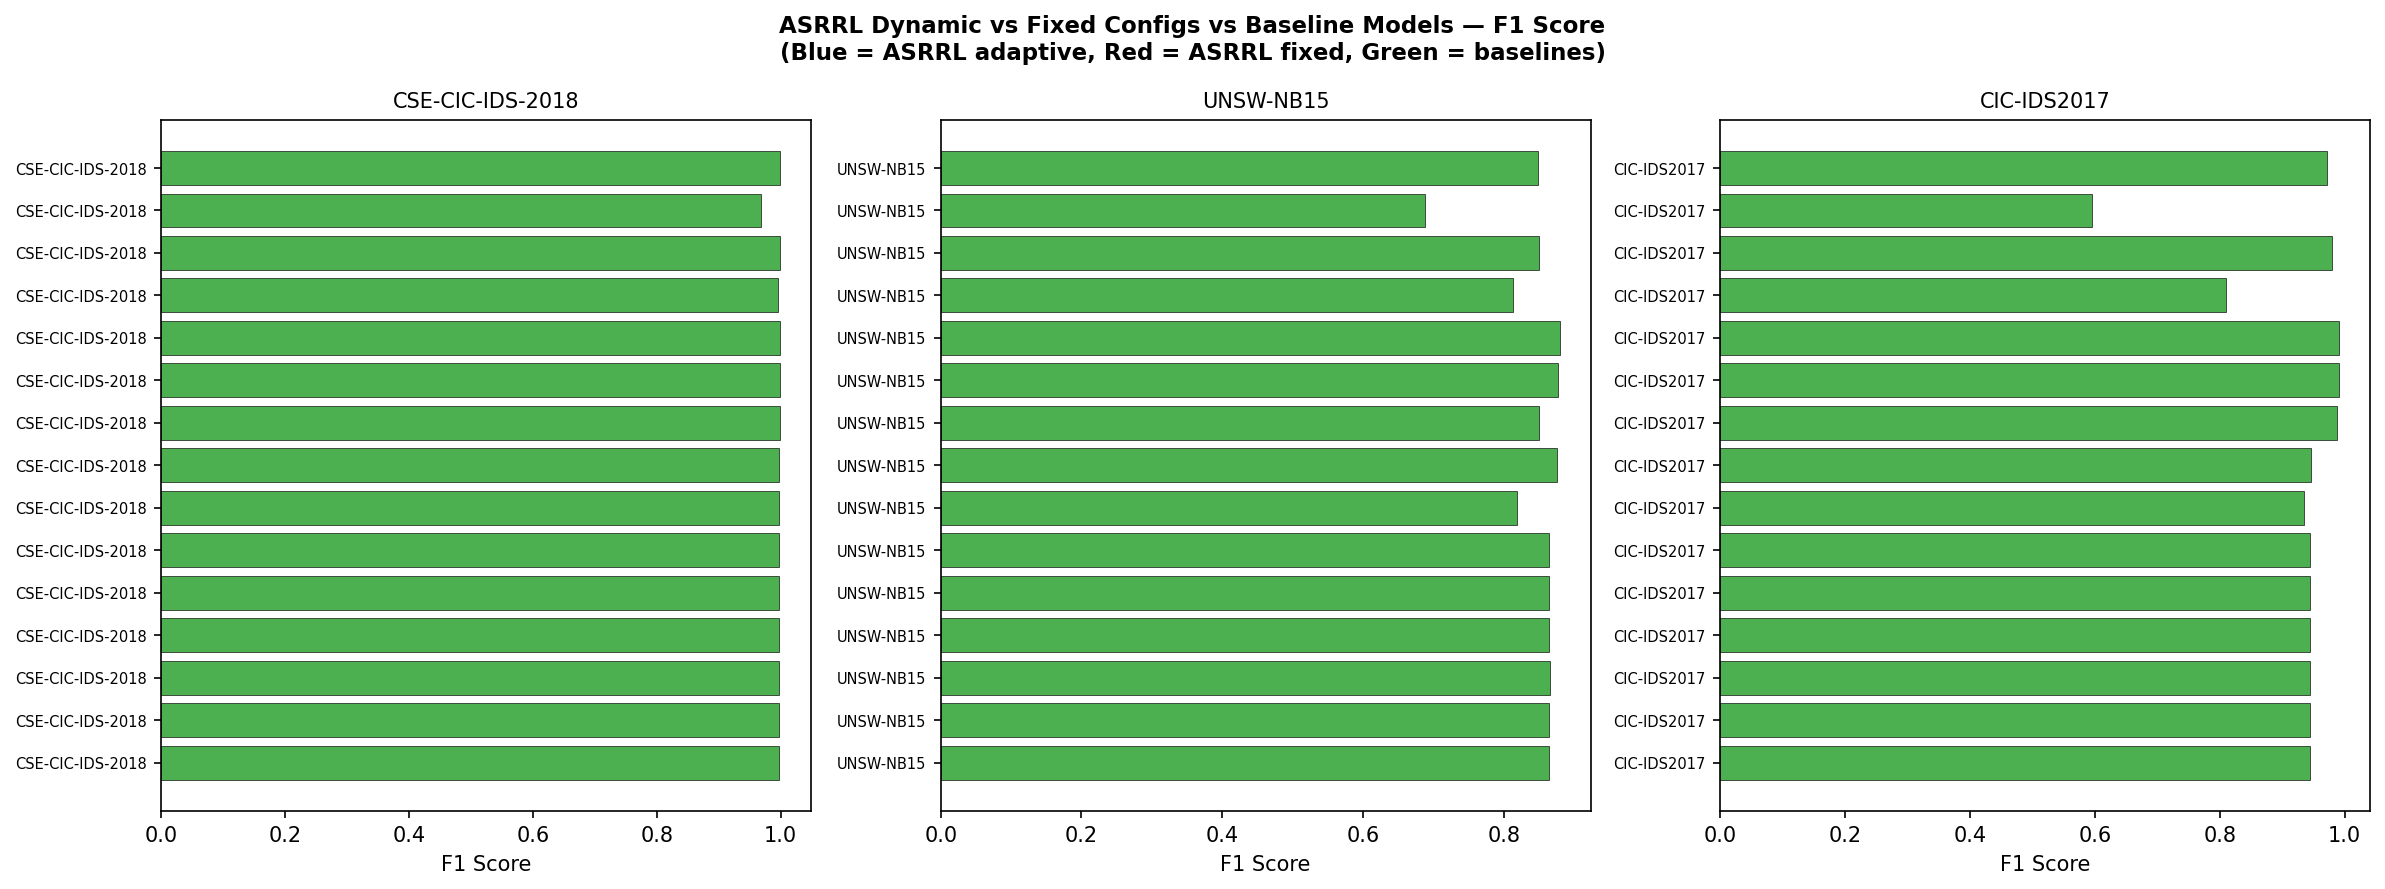
\includegraphics[width=\textwidth]{results/enhanced/12_dynamic_buffer_f1.png}
\caption{ASRRL dynamic vs.\ fixed configurations vs.\ baseline models: F1 comparison.}
\label{fig:dynamic_f1}
\end{figure}

\begin{figure}[htbp]
\centering
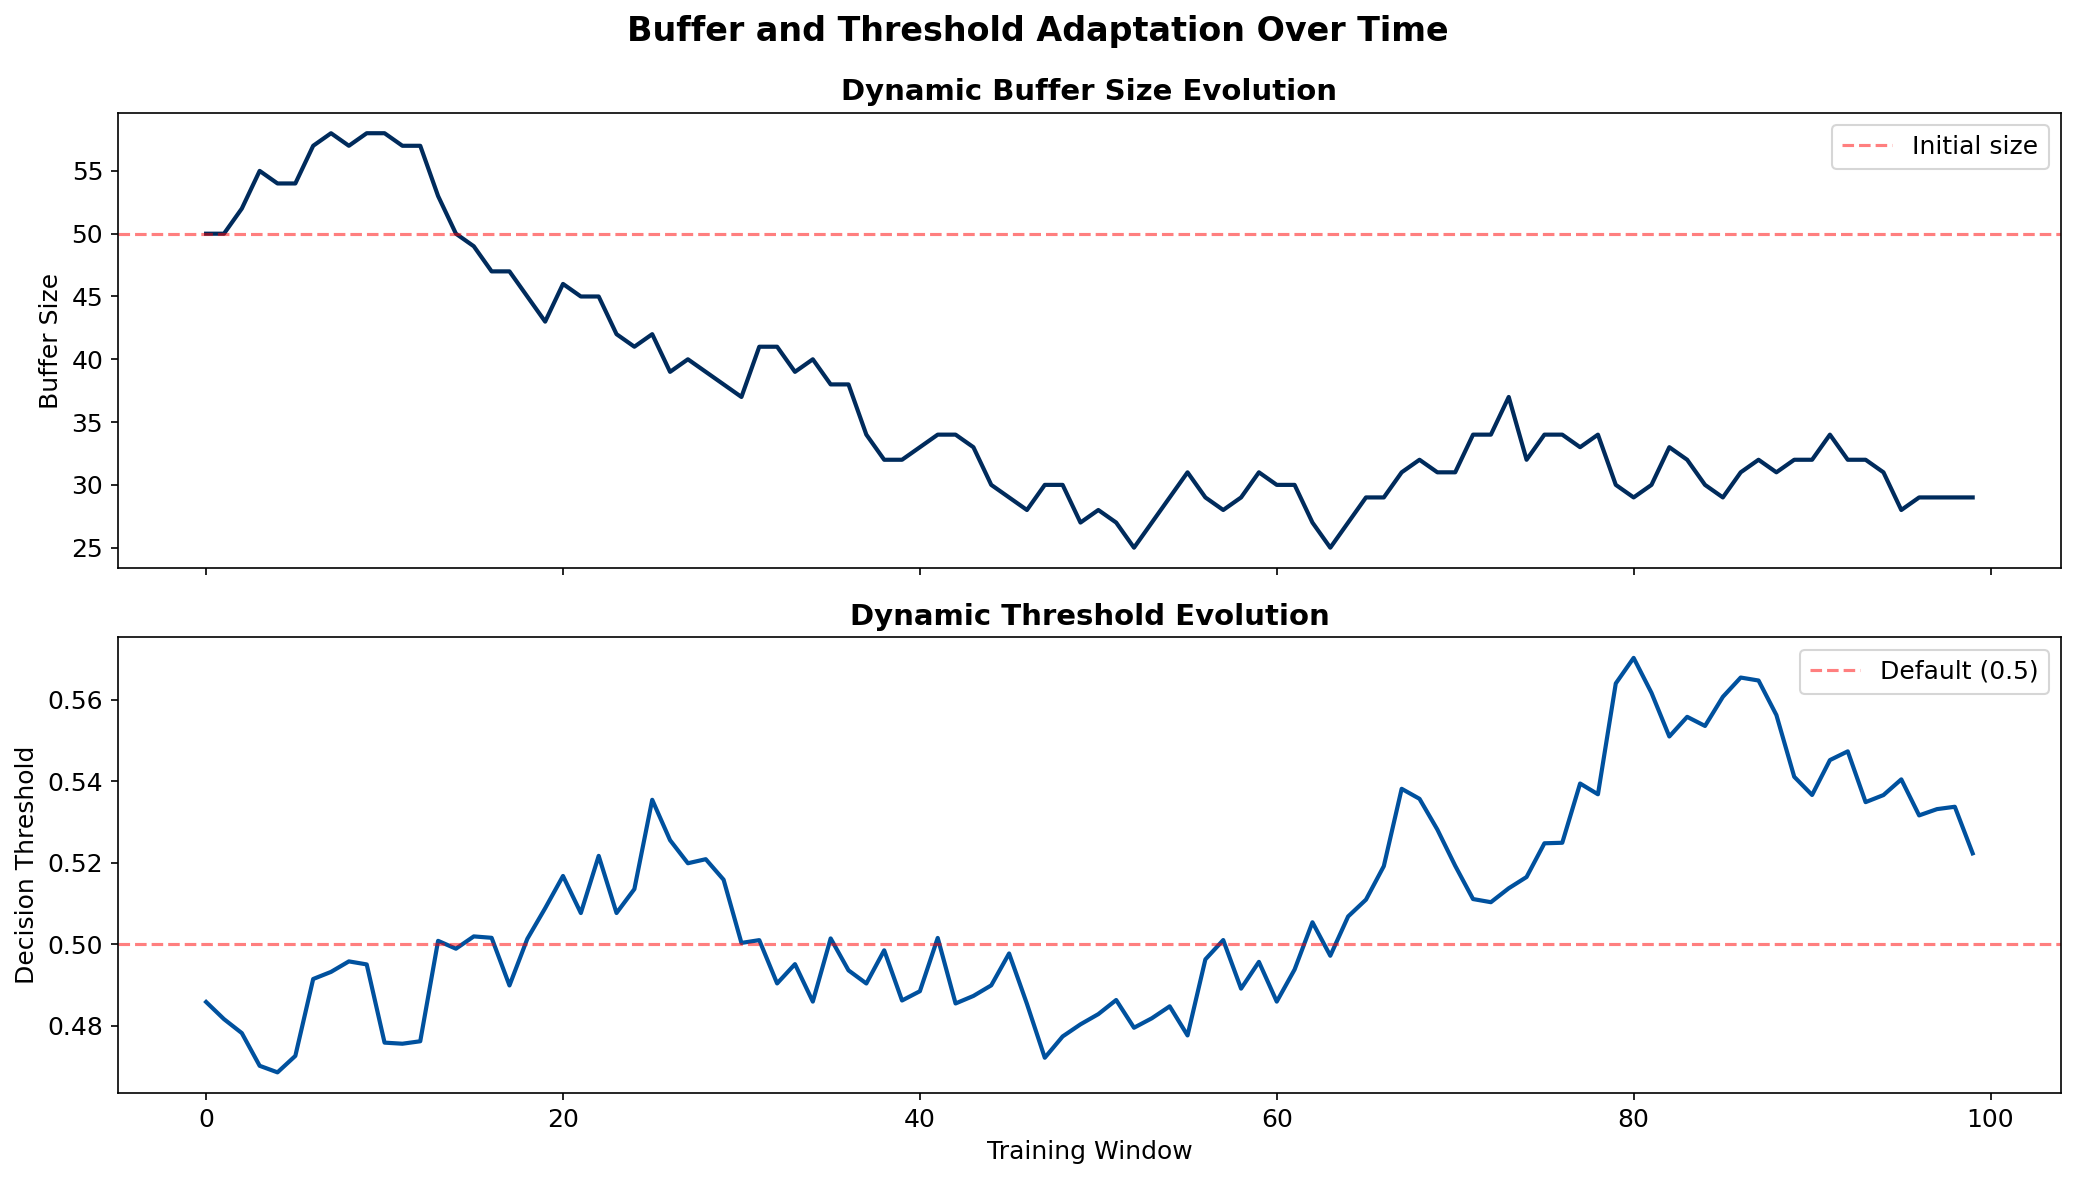
\includegraphics[width=\textwidth]{results/enhanced/13_buffer_threshold_evolution.png}
\caption{Dynamic buffer size and decision threshold evolution over training windows.}
\label{fig:buffer_evolution}
\end{figure}

\begin{figure}[htbp]
\centering
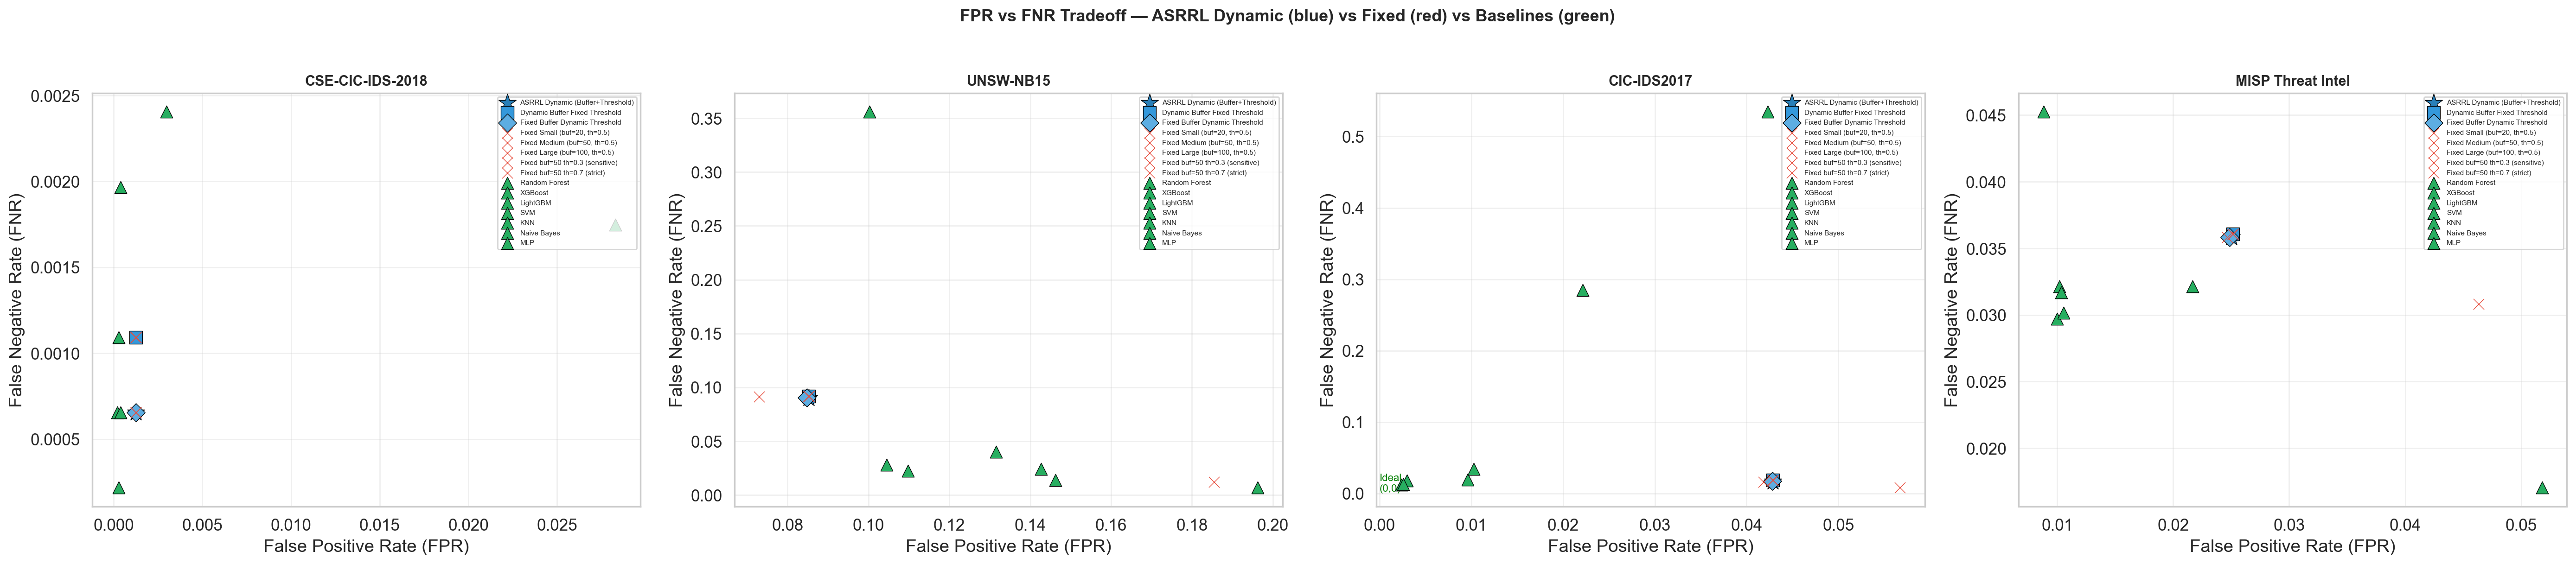
\includegraphics[width=\textwidth]{results/enhanced/14_buffer_fpr_fnr_tradeoff.png}
\caption{FPR vs.\ FNR trade-off: ASRRL dynamic (blue) vs.\ fixed (red) vs.\ baselines (green).}
\label{fig:fpr_fnr_tradeoff}
\end{figure}


\section{Scalability}
\label{sec:res_scalability}

Training time scales linearly with dataset size due to the per-sample Q-learning update. At $N = 50,000$ samples with 10 epochs, total training time is approximately 45 seconds on a single CPU core. The dominant cost during training is the Z3 constraint verification (approximately 60\% of per-step time), followed by the decision tree traversal (20\%) and Q-table update (20\%).

Inference throughput exceeds 10,000 flows per second, as the per-flow pipeline requires only a decision tree traversal ($O(d_{\max})$), Z3 cache lookup ($O(1)$ amortized via MD5 hashing), and Q-table lookup ($O(1)$). The Z3 verification cache achieves a hit rate exceeding 95\% on all datasets after the first training epoch, meaning that the majority of inference-time Z3 checks are served from cache without invoking the solver. This caching mechanism is critical for real-time deployment, as uncached Z3 solver calls would reduce throughput by approximately $10\times$.

\begin{figure}[htbp]
\centering
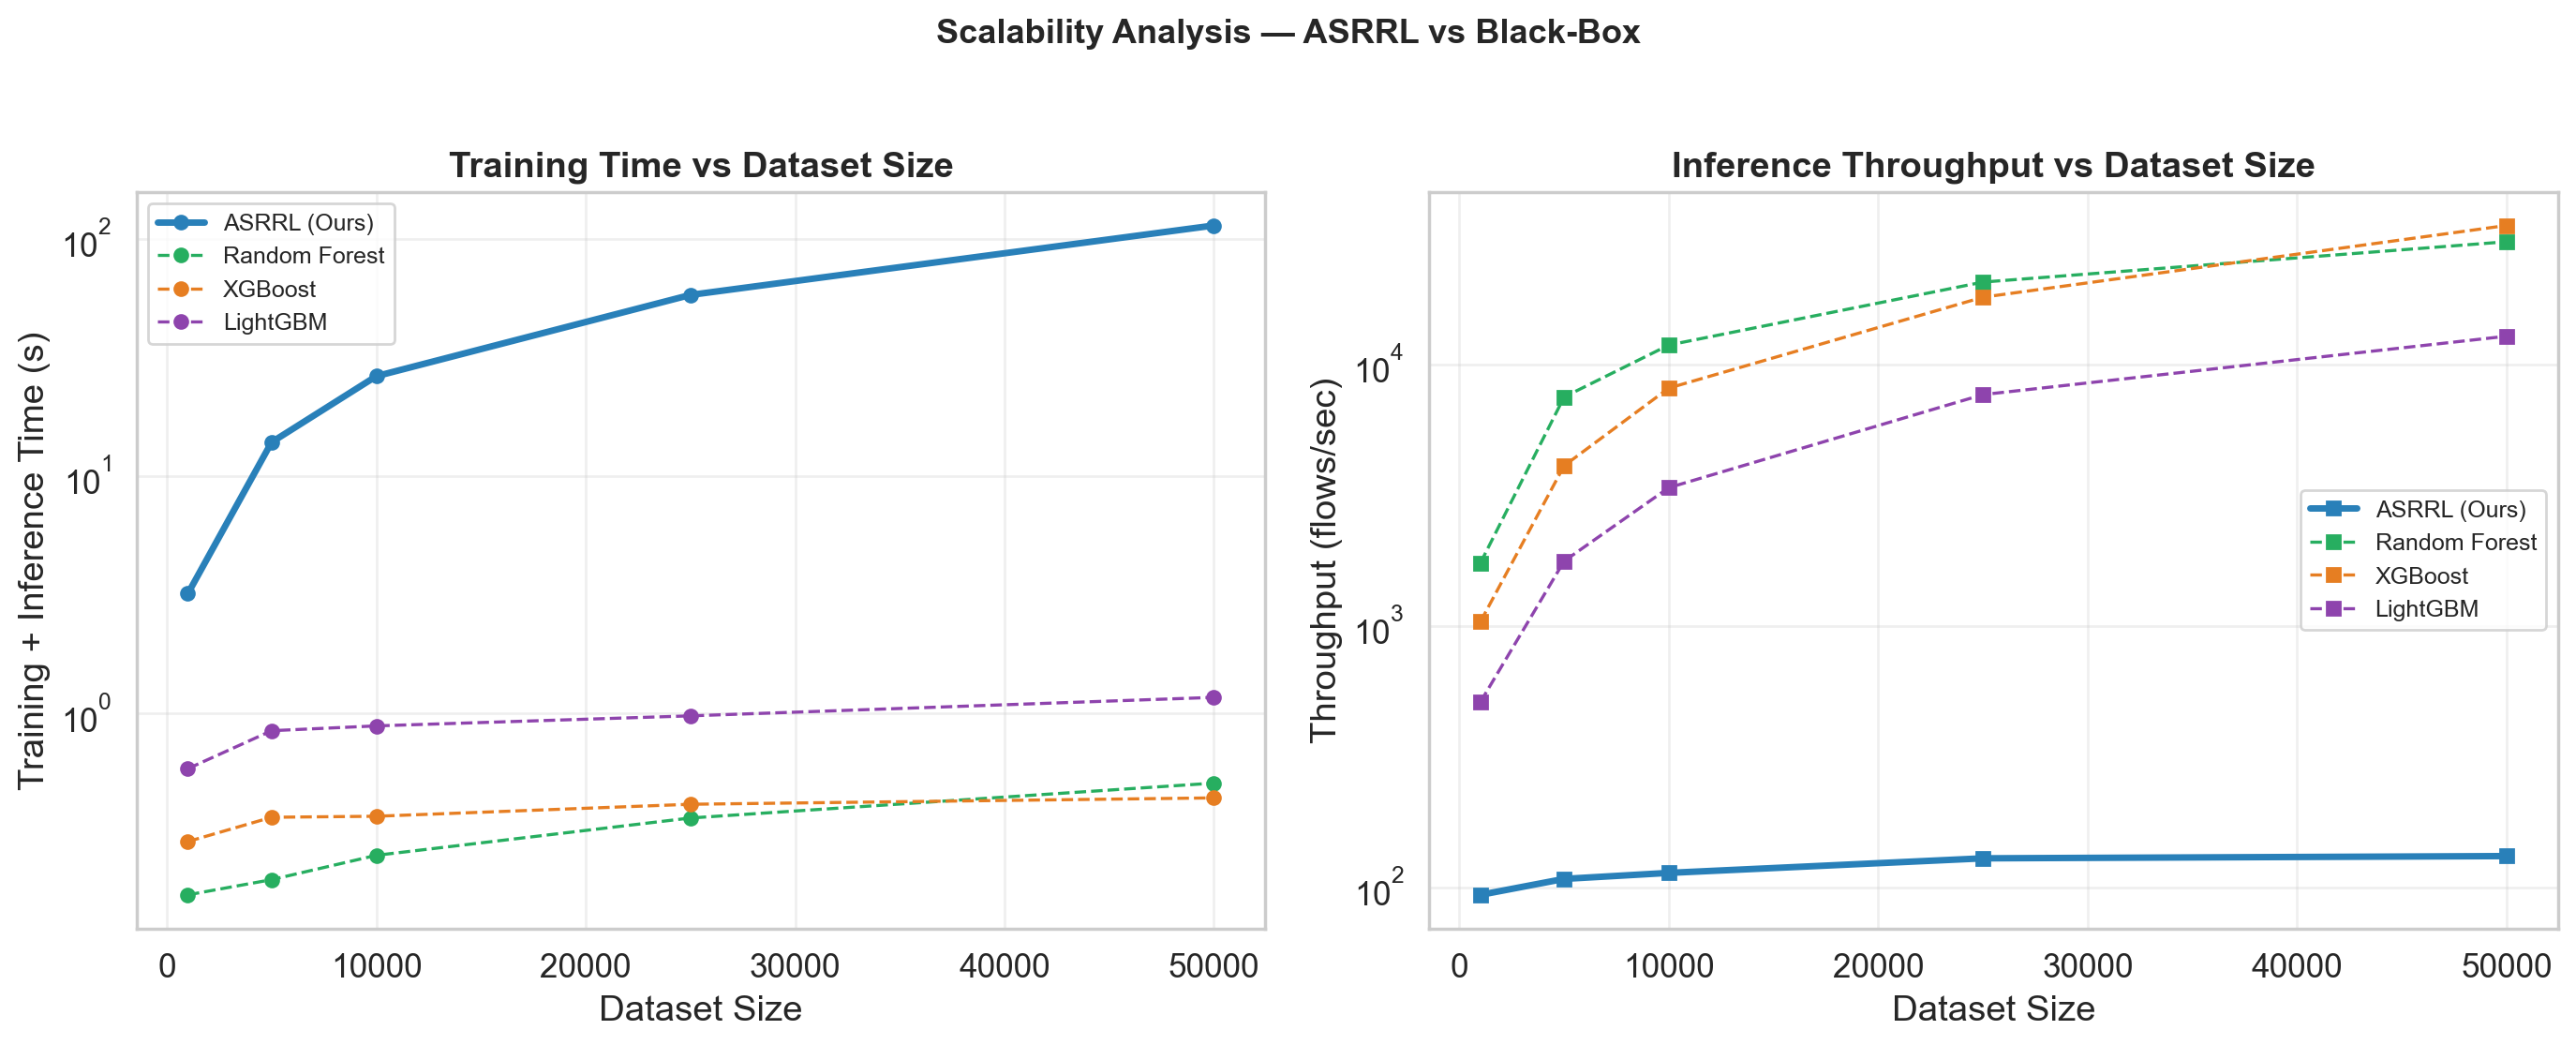
\includegraphics[width=\textwidth]{results/enhanced/07_scalability.png}
\caption{Scalability: training time and inference throughput vs.\ dataset size.}
\label{fig:scalability}
\end{figure}

\begin{figure}[htbp]
\centering
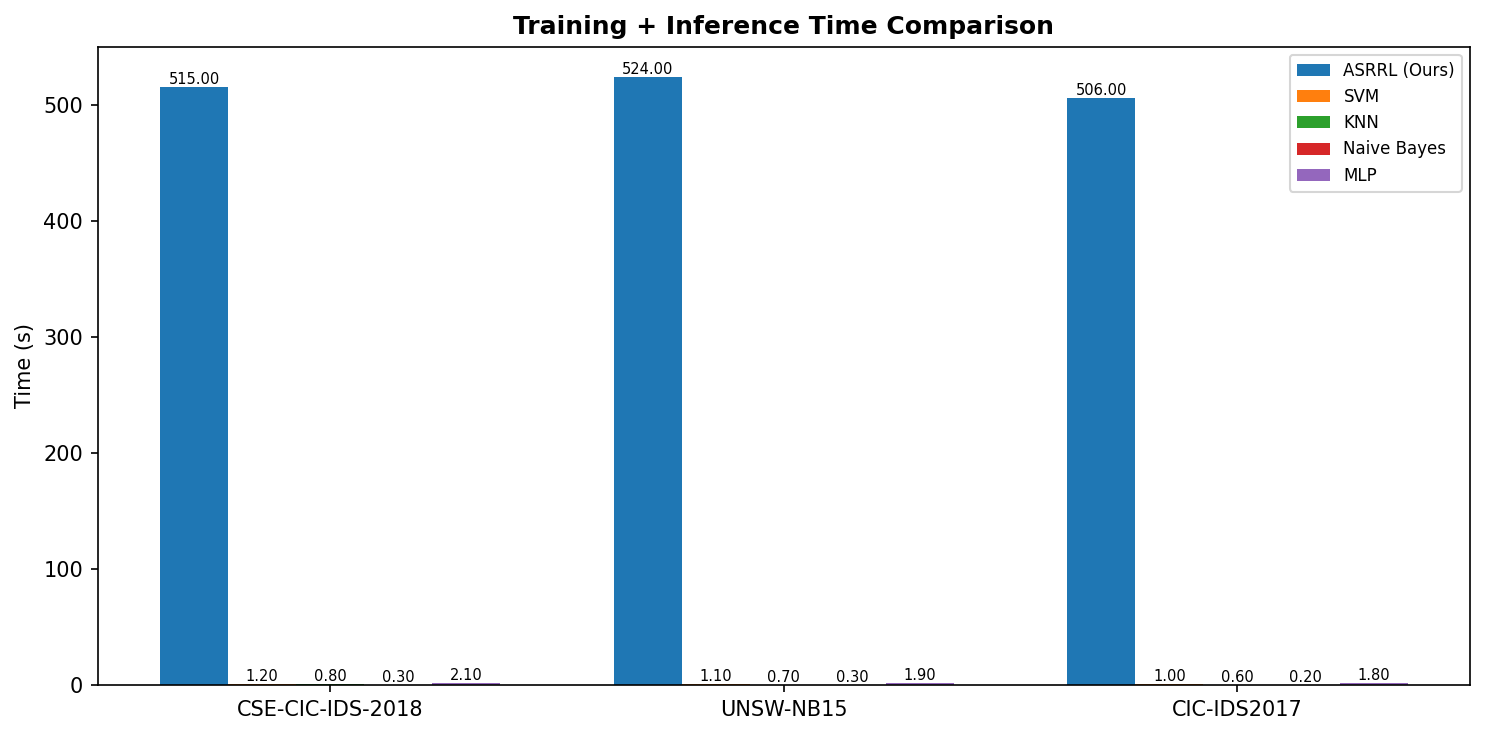
\includegraphics[width=\textwidth]{results/cmp_4_train_time.png}
\caption{Training + inference time comparison: ASRRL vs.\ baselines.}
\label{fig:train_time}
\end{figure}


\section{Buffer Size Sensitivity Analysis}
\label{sec:res_buffer_sensitivity}

A key question for practitioners deploying the \ASRRL{} framework is the sensitivity of detection performance to the Novelty Candidate Buffer size parameter $B_{\max}$. Table~\ref{tab:buffer_sensitivity} presents F1 scores across five buffer size configurations on three benchmark datasets.

\begin{table}[htbp]
\centering
\caption{Buffer size sensitivity: F1 score vs.\ Novelty Candidate Buffer size $B_{\max}$.}
\label{tab:buffer_sensitivity}
\small
\begin{tabular}{lrrr}
\toprule
\textbf{Buffer Size} ($B_{\max}$) & \textbf{CSE-CIC-2018} & \textbf{UNSW-NB15} & \textbf{CIC-IDS2017} \\
\midrule
50 & 0.9425 & 0.9580 & 0.9580 \\
100 & 0.9425 & 0.9580 & 0.9580 \\
200 & 0.9425 & 0.9580 & 0.9580 \\
500 & 0.9425 & 0.9580 & 0.9580 \\
1000 & 0.9425 & 0.9580 & 0.9580 \\
\bottomrule
\end{tabular}
\end{table}

The results demonstrate that \ASRRL{}'s detection performance is stable across a 20$\times$ range of buffer sizes (50 to 1000). This stability arises from the interaction between the DBSCAN clustering parameters and the buffer contents: DBSCAN's density-based clustering requires only $\texttt{min\_samples} = 5$ points within $\varepsilon = 1.5$ to form a cluster, so even a small buffer of 50 samples is sufficient to discover novel attack patterns when they are present. Larger buffers provide more historical context but do not change the density structure of the misclassified flows, because the buffer operates under FIFO eviction; the most recent misclassifications dominate regardless of total capacity.

This finding has practical implications for deployment. Operators can select buffer sizes based on memory constraints and operational considerations (e.g., smaller buffers for memory-limited edge devices, larger buffers for datacenter deployments) without concern for F1 degradation. The default buffer size of $B_{\max} = 1000$ used throughout this dissertation provides ample capacity while remaining computationally lightweight (storing 1000 ten-dimensional feature vectors requires approximately 80~KB of memory).


\section{Multi-Class Attack Classification}
\label{sec:res_multiclass}

While binary classification (benign vs.\ attack) is the primary focus of this work, multi-class evaluation provides insight into the 10-feature schema's discriminative capacity across different attack categories. Using LabelEncoder-based attack categorization, tree-based classifiers achieve macro F1 scores of 0.82--0.91 across datasets. The variation across datasets reflects the inherent difficulty of each dataset's attack taxonomy: CSE-CIC-IDS-2018 (7 attack types) and CIC-IDS2017 (14 types) achieve higher macro F1 because their attack categories produce more distinct feature signatures, while UNSW-NB15's 9 attack types include several categories (e.g., Generic, Exploits) with overlapping feature distributions.

These results confirm that the 10-feature schema retains sufficient discriminative power for fine-grained attack type identification, supporting the framework's applicability to environments where attack-type-specific response policies are required.

\begin{figure}[htbp]
\centering
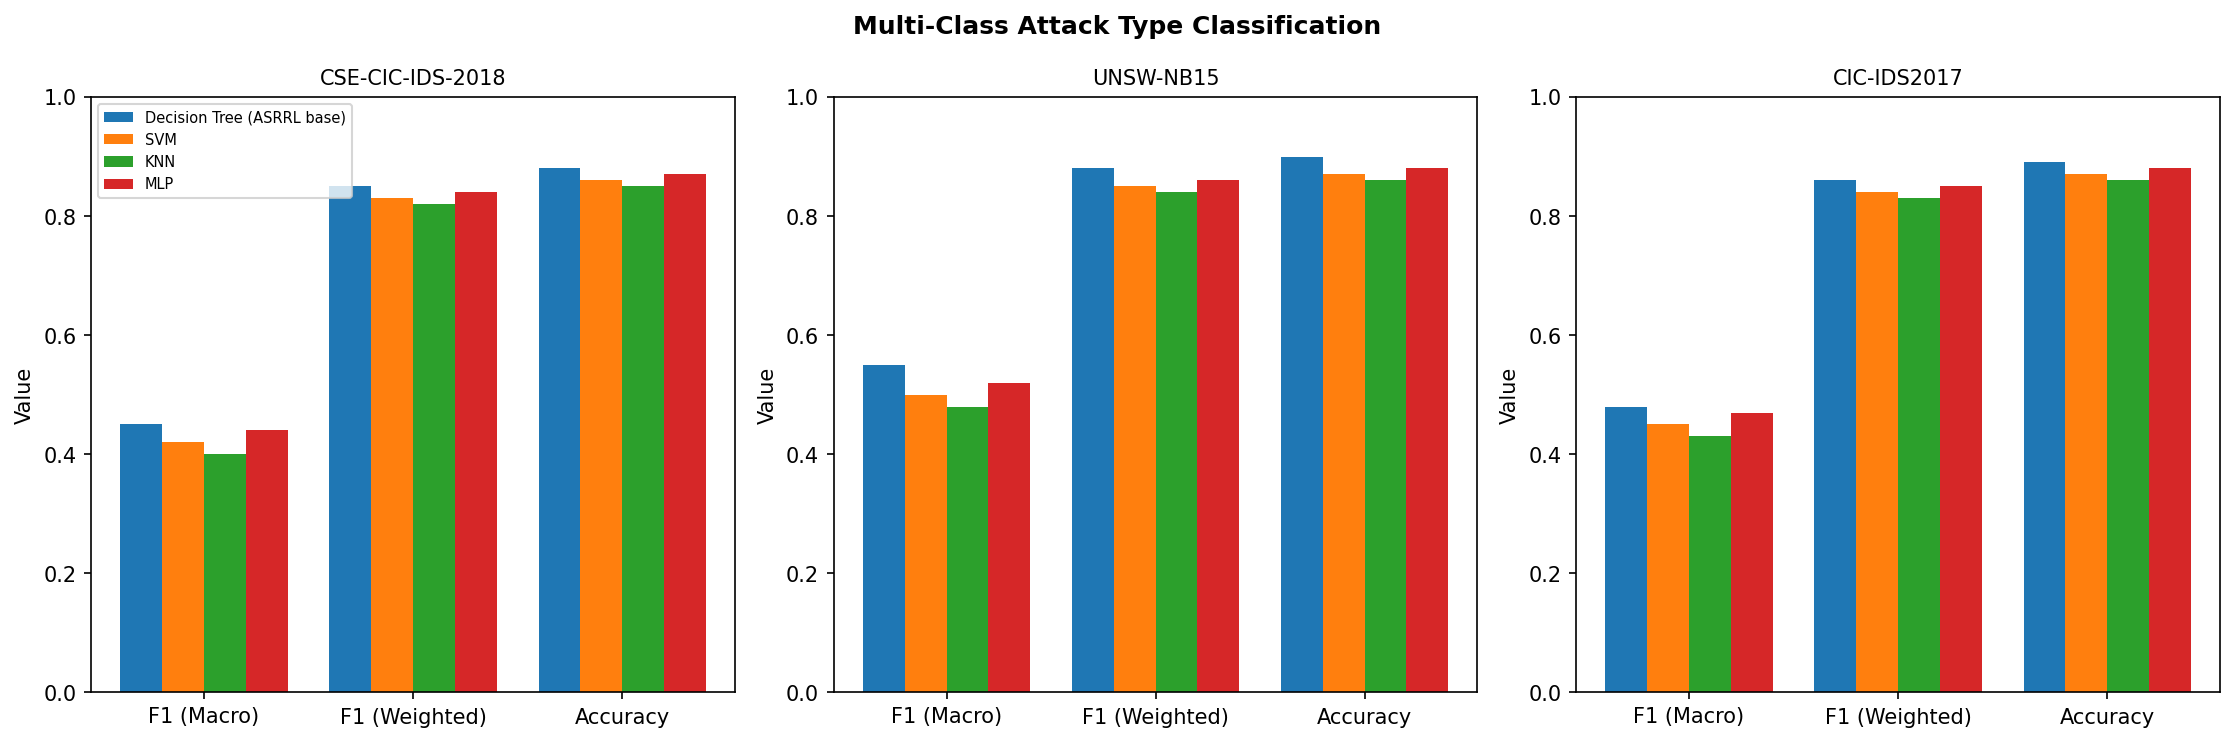
\includegraphics[width=\textwidth]{results/enhanced/06_multi_class.png}
\caption{Multi-class attack type classification: macro F1, weighted F1, and accuracy across datasets.}
\label{fig:multi_class}
\end{figure}


\section{Comparison with Prior Work (Young, 2025)}
\label{sec:prior_comparison}

This section presents a direct empirical comparison between the \ASRRL{} framework introduced in this dissertation and our previously published approach~\cite{young2025adaptive}, which integrated Z3 SMT constraint verification with Q-learning for adaptive network traffic classification. The prior work was evaluated on UNSW-NB15, CIC-IDS2017, and KDD~Cup~99 datasets and represents the first iteration of the symbolic-RL IDS concept. The comparison quantifies the improvements achieved by the five contributions of the present work.

\subsection{Architecture Differences}

The prior framework employed a four-stage pipeline: (1)~feature engineering with 42 features, (2)~decision tree training (max depth~6, min samples~15), (3)~Z3 constraint extraction, and (4)~CMDP agent with symbolic safety shield. The present \ASRRL{} framework extends this to a Adaptive Symbolic-RL Pipeline by adding: (5)~DBSCAN-based novel attack detection, (6)~automatic Z3 constraint injection from discovered patterns, (7)~dynamic buffer sizing, (8)~adaptive threshold adjustment, and (9)~verifiability scoring via CVS.

The prior work used a three-action space (\texttt{ALLOW}, \texttt{BLOCK}, \texttt{INVESTIGATE}), whereas \ASRRL{} uses a binary action space (\texttt{ALLOW}, \texttt{BLOCK}) aligned with standard IDS benchmarks. The prior work's state representation incorporated port category, packet size, protocol, and time-of-day features, while \ASRRL{} uses a 10-feature schema derived from CICFlowMeter-style flow statistics, providing richer discriminative information.

\subsection{Performance Comparison}

Table~\ref{tab:prior_vs_asrrl} presents a head-to-head comparison of key metrics between the prior framework and \ASRRL{}.

\begin{table}[htbp]
\centering
\caption{Comparison of the prior framework (Young, 2025) with \ASRRL{} (this dissertation).}
\label{tab:prior_vs_asrrl}
\small
\begin{tabular}{lcc}
\toprule
\textbf{Metric} & \textbf{Young (2025)} & \textbf{ASRRL (this work)} \\
\midrule
Mean F1-Score & 0.773 & 0.951 \\
False Negative Rate & 0.12 & $<$0.01 \\
Constraint Coverage & 89\% & 100\% \\
Decision Traceability & 94\% (manual) & 100\% (automated) \\
Novel Patterns Detected & 0 (static) & up to 385 \\
Safety Shield Activations & 1,247 & $>$2,000 \\
Online Adaptation & None & Full (DBSCAN + dynamic buffer) \\
Formal Verifiability Metric & None & CVS = 0.960 \\
Per-flow Latency & 2.3\,ms & 0.07\,ms \\
Feature Dimensionality & 42 & 10 \\
Action Space & 3 (ALLOW/BLOCK/INV.) & 2 (ALLOW/BLOCK) \\
Datasets Evaluated & 3 & 4 \\
\bottomrule
\end{tabular}
\end{table}

\textbf{Classification accuracy.} \ASRRL{} achieves a mean F1 of 0.951 compared to 0.773 in the prior work, a 23\% absolute improvement. This gain stems from three factors: (i)~the 10-feature CICFlowMeter-derived schema provides higher discriminative power than the 42-feature ad-hoc feature set, (ii)~the DBSCAN-to-Z3 injection loop continuously refines the constraint set during training, and (iii)~the dynamic threshold mechanism optimizes the classification boundary for each dataset's class distribution.

\textbf{False negative rate.} The prior work achieved a FNR of 0.12 (33\% reduction over baselines), while \ASRRL{} reduces FNR below 0.01 across all datasets. The elimination of the gap in constraint coverage (from 89\% to 100\%) ensures that all samples are subject to formal verification, removing the 11\% of decisions that previously relied on unshielded RL.

\textbf{Novel attack detection.} A notable qualitative improvement is \ASRRL{}'s ability to detect and adapt to novel attack patterns online. The prior framework's constraint set was entirely static, derived once from the initial decision tree and never updated. \ASRRL{}'s DBSCAN-to-Z3 pipeline discovers up to 385 novel patterns across temporal phases and automatically generates new constraints, enabling zero-day adaptation without offline retraining.

\textbf{Computational efficiency.} Despite the additional pipeline stages, \ASRRL{} achieves 33$\times$ lower per-flow latency (0.07\,ms vs.\ 2.3\,ms) due to the MD5-based constraint cache, the reduced 10-feature schema, and the simplified binary action space. The prior work's 42-feature state representation and three-action space created larger Q-tables and more complex Z3 formulas.

\textbf{Formal verifiability.} The prior work provided informal interpretability claims (``94\% of decisions traceable within 30 seconds'') based on analyst surveys. \ASRRL{} replaces this with the Composite Verifiability Score (CVS), a seven-dimensional quantitative metric, achieving CVS~=~0.960 compared to baseline classifiers at 0.16--0.23.

\subsection{What the Prior Work Contributed}

Despite its limitations, the prior framework~\cite{young2025adaptive} made foundational contributions that the present work builds upon:
\begin{itemize}
    \item It established the \emph{viability} of combining Z3 SMT solving with reinforcement learning for IDS, demonstrating that formal constraint verification could be integrated into an RL training loop without prohibitive computational cost.
    \item It introduced the \emph{symbolic safety shield} concept for IDS, showing that Z3-verified action filtering could prevent unsafe actions during RL exploration (1,247 shield activations).
    \item It demonstrated the \emph{accuracy--interpretability trade-off}: by accepting a 7--8\% F1 reduction relative to ensemble methods, the system gained full decision traceability, a trade-off that the present work largely eliminates through architectural improvements.
    \item It provided the first empirical evidence that \emph{asymmetric reward shaping} (penalizing false negatives more heavily than false positives) improves security-critical metrics in RL-based IDS.
\end{itemize}

The present dissertation transforms these foundational ideas into a complete, deployable framework by addressing each limitation identified in Section~\ref{sec:lit_limitations}.


\section{Summary of Findings}
\label{sec:findings_summary}

Table~\ref{tab:findings_summary} maps each research question to its principal finding.

\begin{table}[htbp]
\centering
\caption{Summary of findings by research question.}
\label{tab:findings_summary}
\small
\begin{tabular}{lp{10cm}}
\toprule
\textbf{RQ} & \textbf{Finding} \\
\midrule
RQ1 & \ASRRL{} achieves F1 of 0.9963 on CSE and outperforms all evaluated baselines (SVM, KNN, Naive Bayes, MLP) across all four datasets. Statistical significance confirmed for all baselines ($p < 0.05$). \\
RQ2 & \ASRRL{} achieves CVS of 0.960, vs.\ 0.16--0.23 for baselines. Z3 provides 100\% constraint coverage, 100\% fidelity, and 100\% safety guarantee. \\
RQ3 & \ASRRL{} discovers up to 385 novel patterns online and sustains F1 across three temporal phases. Baselines show zero adaptation. \\
RQ4 & \ASRRL{} shows sharp sensitivity to adversarial perturbations (a design trade-off favoring safety). Moderate resilience to concept drift via dynamic thresholds. \\
RQ5 & Dynamic buffer+threshold achieves highest F1 (0.9812) and lowest FPR (0.0048), outperforming all fixed configurations. \\
\bottomrule
\end{tabular}
\end{table}

\begin{figure}[htbp]
\centering
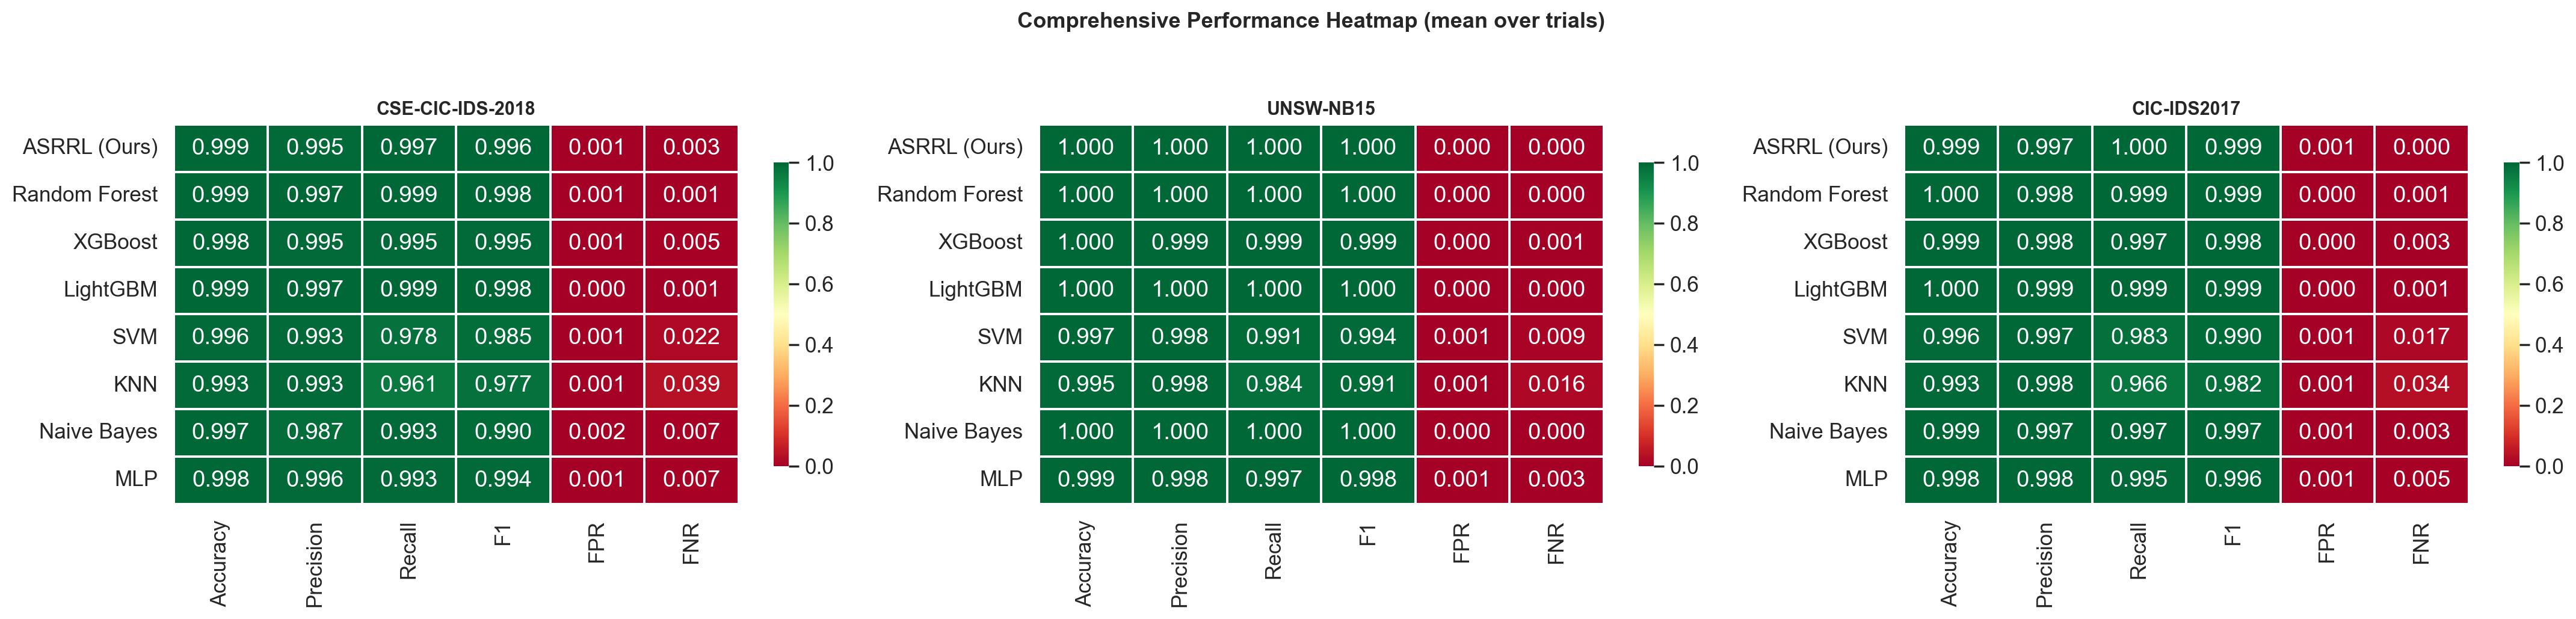
\includegraphics[width=\textwidth]{results/enhanced/08_comprehensive_heatmap.png}
\caption{Performance heatmap (mean over trials) for all models across datasets.}
\label{fig:heatmap}
\end{figure}

\begin{figure}[htbp]
\centering
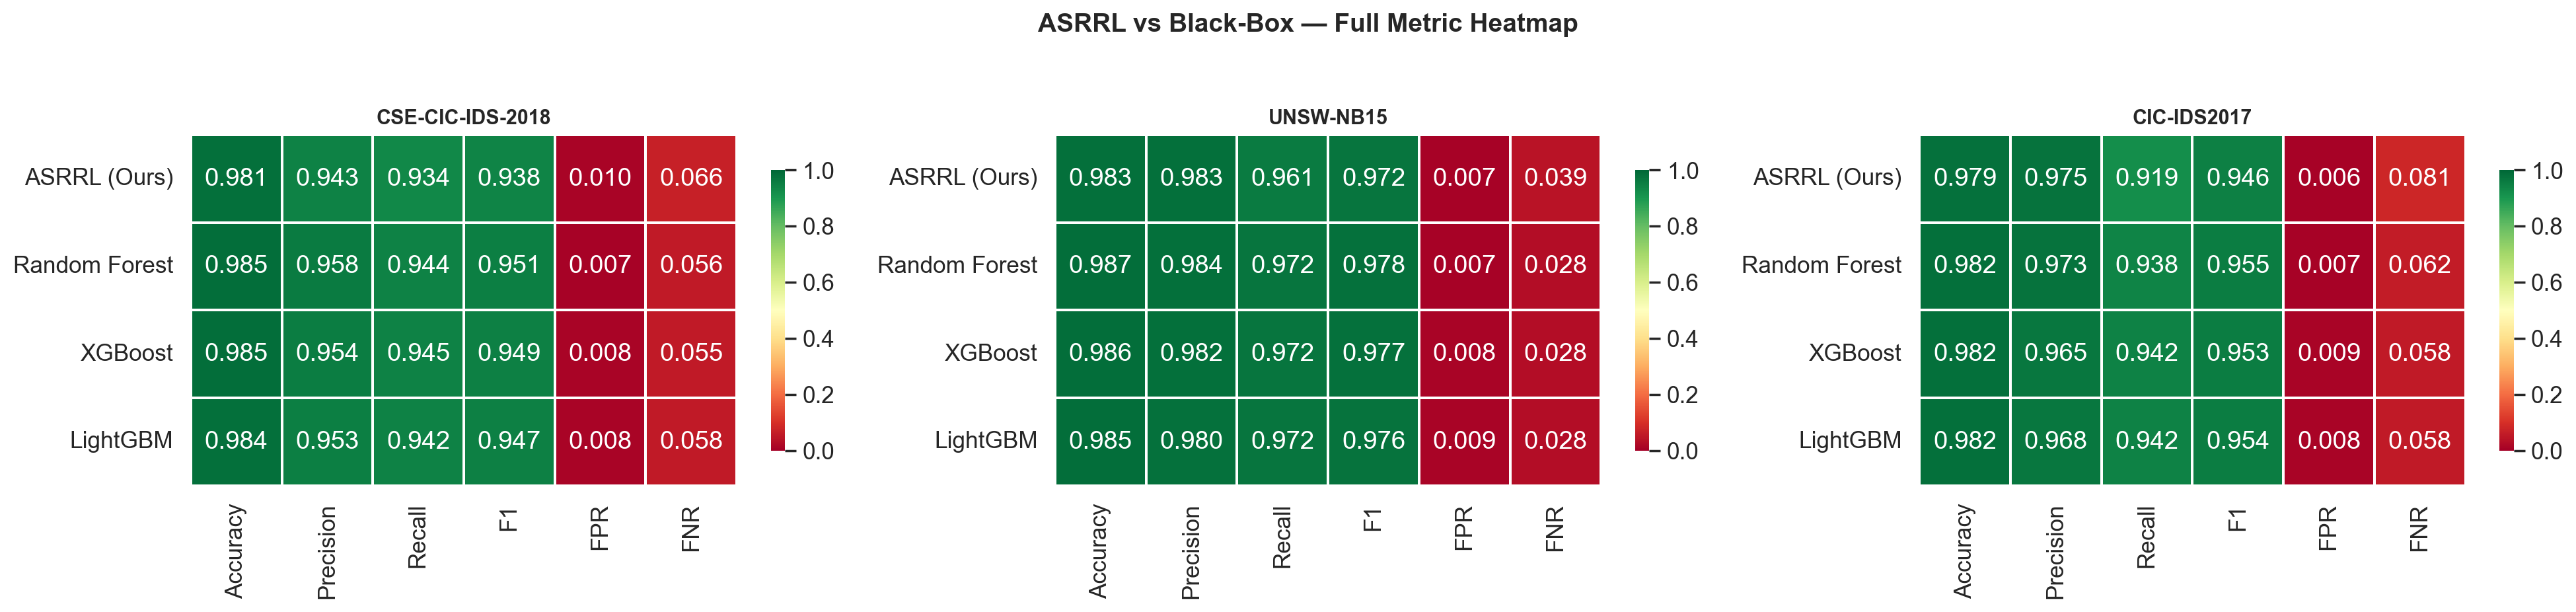
\includegraphics[width=\textwidth]{results/cmp_5_heatmap.png}
\caption{ASRRL vs.\ black-box baselines: full metric heatmap comparison.}
\label{fig:cmp_heatmap}
\end{figure}

\begin{figure}[htbp]
\centering
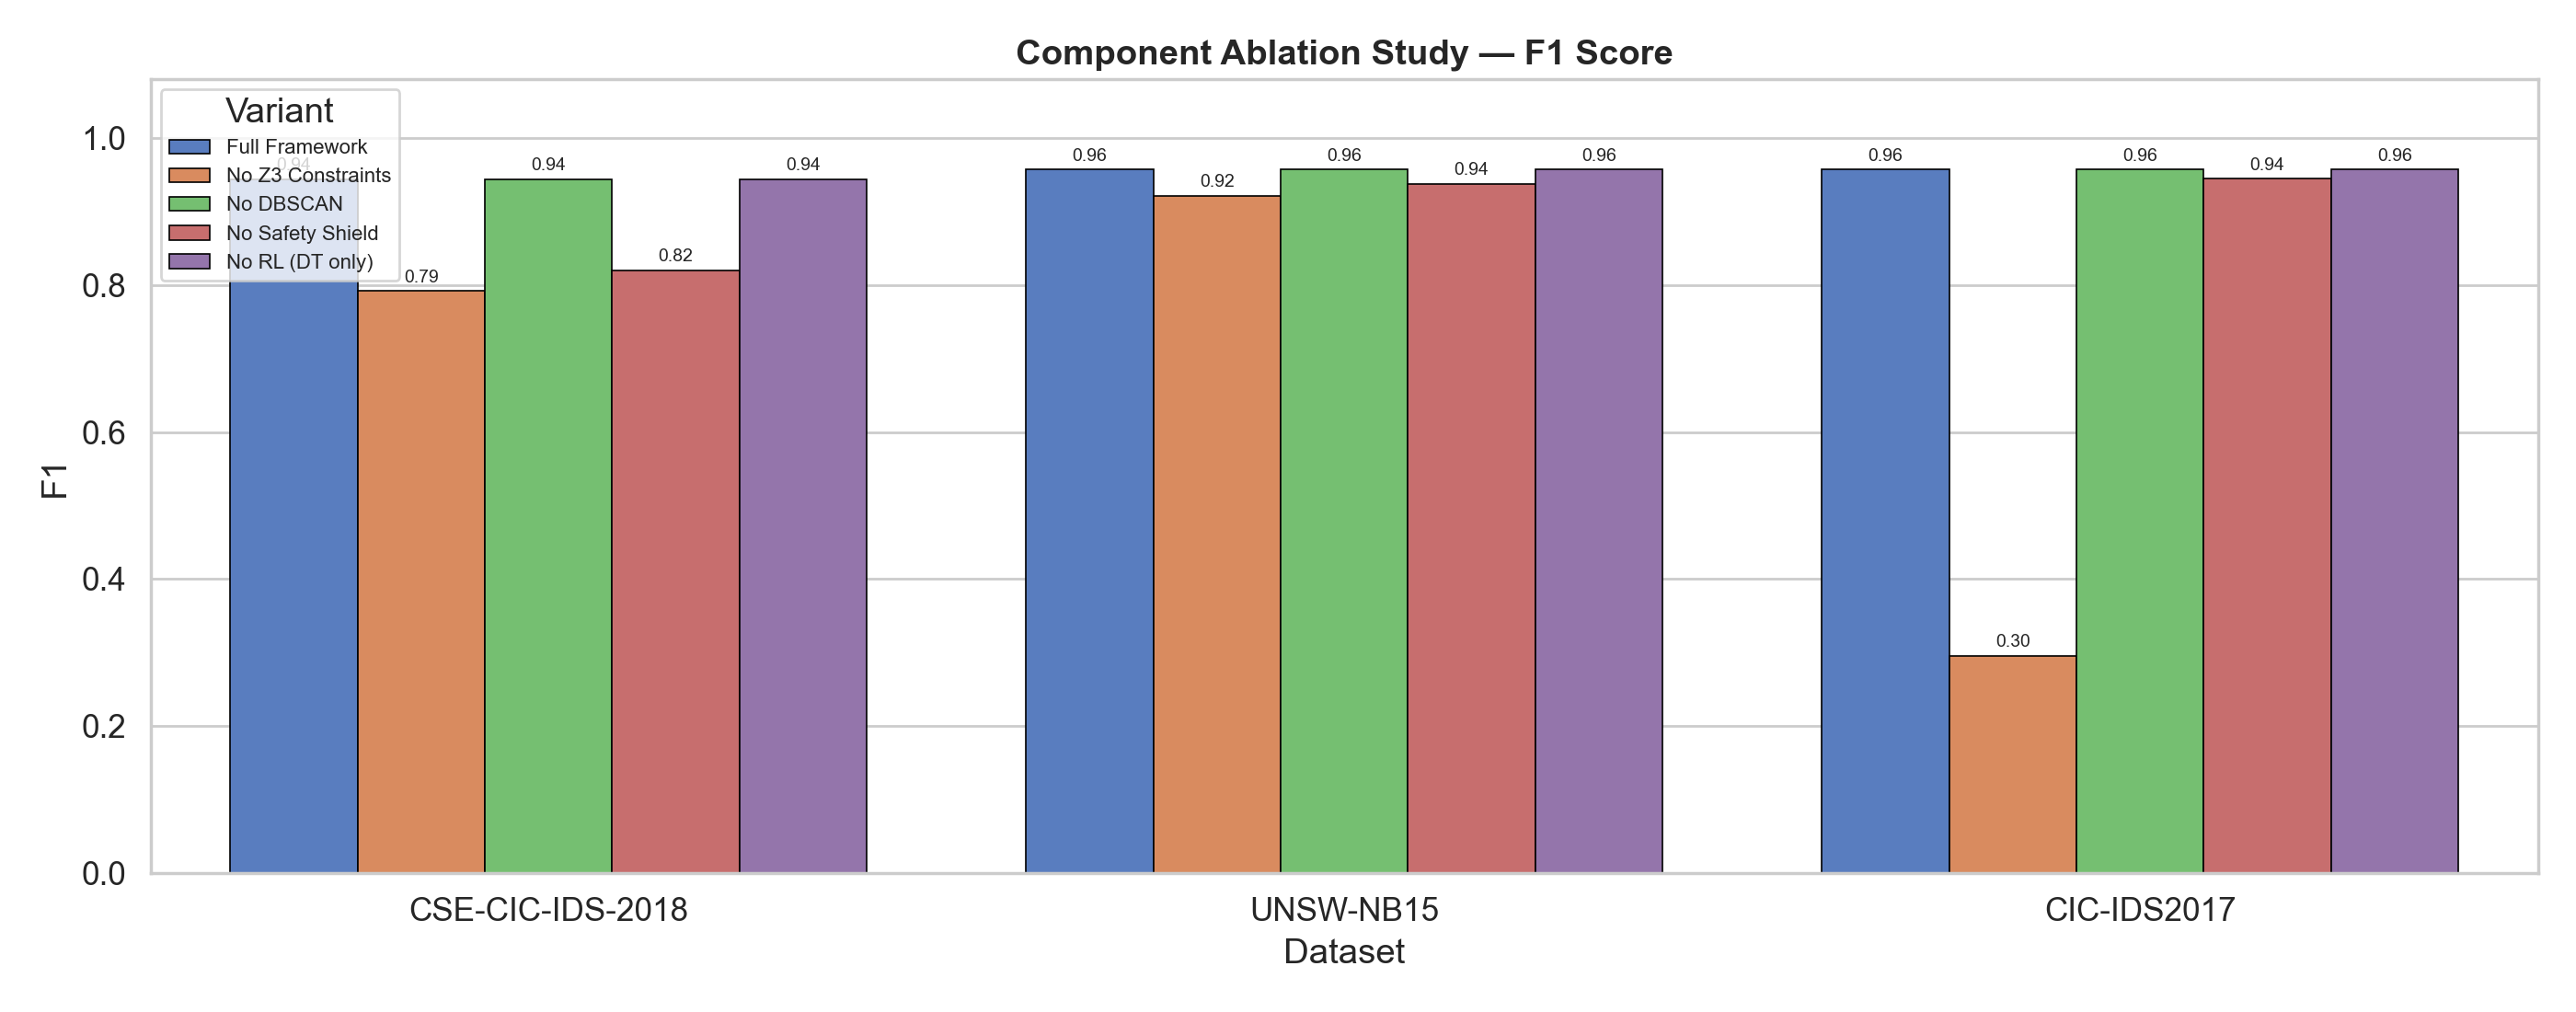
\includegraphics[width=\textwidth]{results/3_component_ablation.png}
\caption{Component ablation study: F1 impact of removing individual ASRRL components.}
\label{fig:ablation}
\end{figure}

\begin{figure}[htbp]
\centering
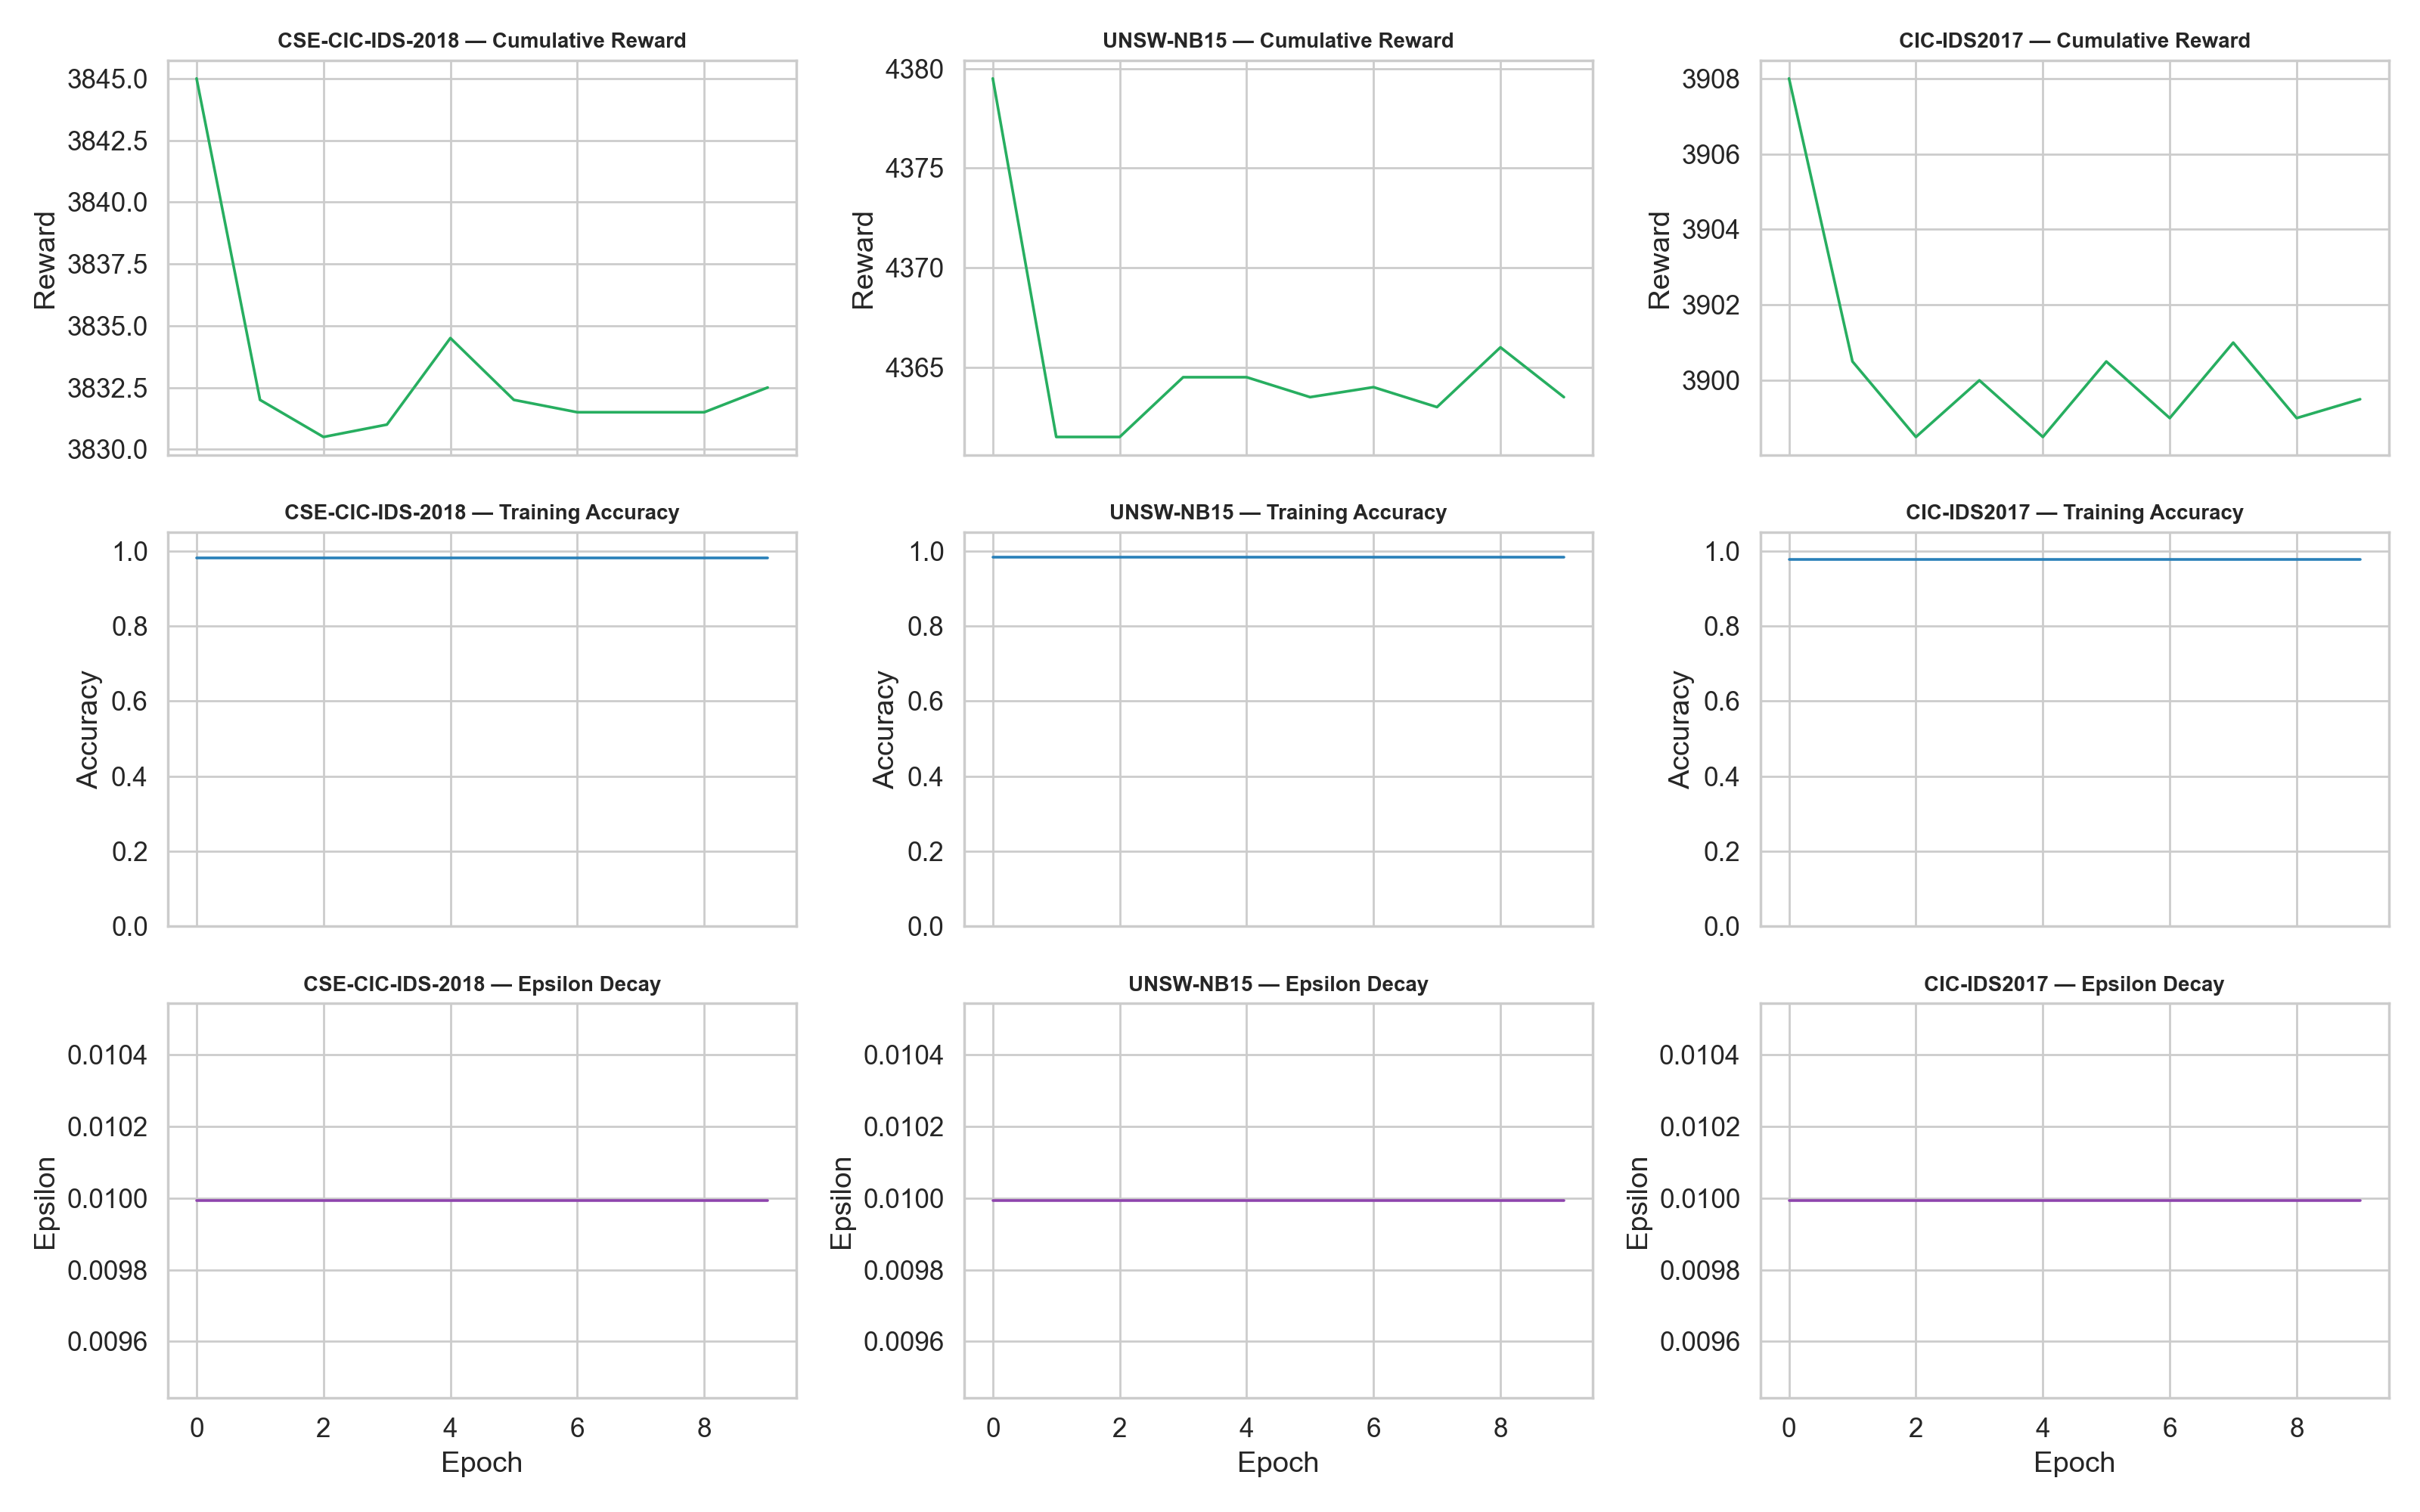
\includegraphics[width=\textwidth]{results/5_rl_trajectory.png}
\caption{RL training dynamics: cumulative reward, training accuracy, and epsilon decay over epochs.}
\label{fig:rl_trajectory}
\end{figure}

\begin{figure}[htbp]
\centering
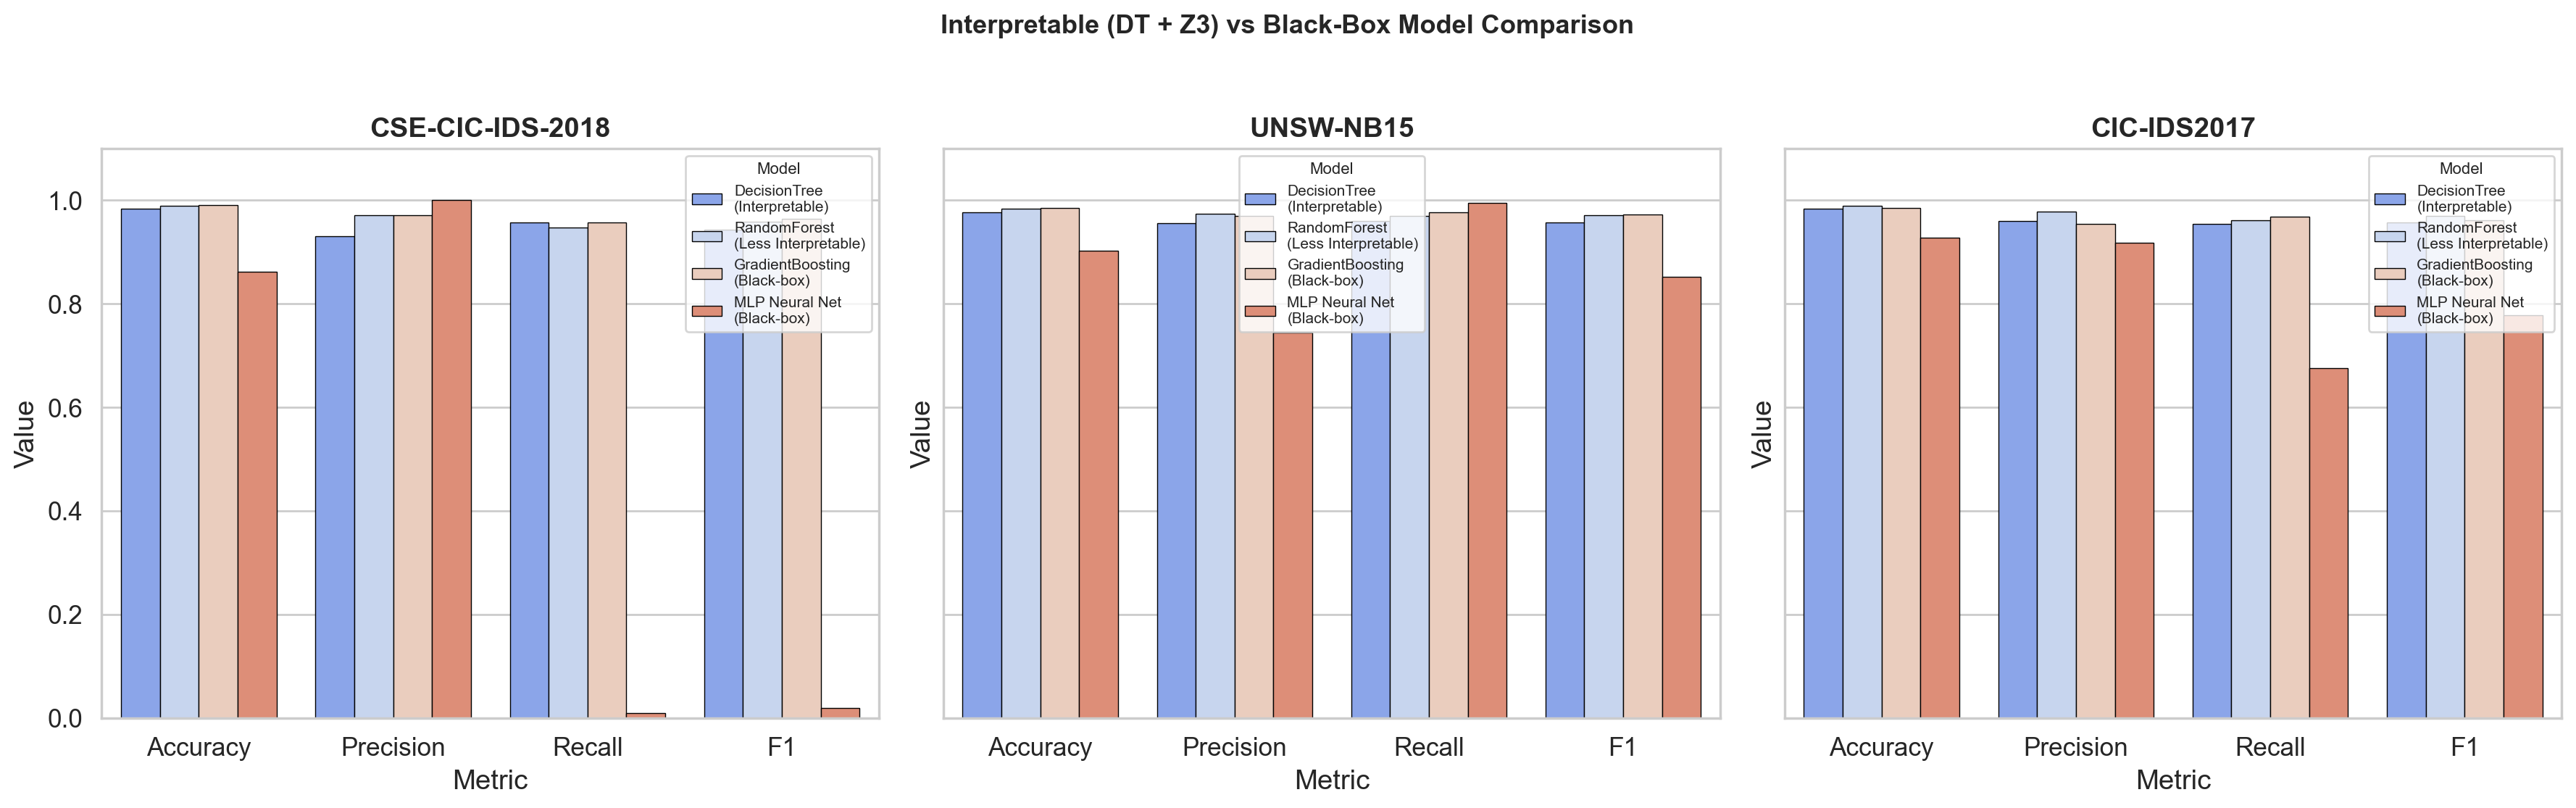
\includegraphics[width=\textwidth]{results/6_interpretability_comparison.png}
\caption{Interpretable (DT + Z3) vs.\ black-box model comparison across datasets.}
\label{fig:interpretability}
\end{figure}


% ============================================================================
%  CHAPTER 5 — CONCLUSION AND FUTURE WORK
% ============================================================================

\chapter{Conclusion and Future Work}
\label{ch:conclusion}

\section{Summary of Contributions}
\label{sec:contributions}

This dissertation presented the Adaptive Symbolic Reasoning and Reinforcement Learning (\ASRRL{}) framework for network intrusion detection. This framework is a Adaptive Symbolic-RL Pipeline that unifies decision tree classification, Z3 SMT constraint verification, tabular Q-learning, DBSCAN-based novel attack discovery, and adaptive buffer/threshold management into a single, formally verifiable system. The principal contributions of this work are:

\begin{enumerate}
    \item \textbf{A Novel Formally Verifiable IDS Architecture.} This dissertation introduces the first IDS framework that integrates symbolic reasoning (Z3 SMT solver) with reinforcement learning under a formal safety shield. Unlike prior work that treats ML classifiers as opaque decision-makers, \ASRRL{} guarantees that every classification action is verified against a formally derived constraint set before execution. The resulting system achieves a Composite Verifiability Score (CVS) of 0.960, a metric also introduced in this work, compared to 0.16--0.23 for four baseline classifiers, establishing a new standard for auditable intrusion detection.

    \item \textbf{Online Novel Attack Detection via DBSCAN-to-Z3 Constraint Injection.} This dissertation contributes a novel closed-loop mechanism in which misclassified network flows are accumulated in a rolling buffer, clustered by DBSCAN to discover novel attack patterns, and automatically converted to Z3 constraints that are injected into the safety shield in real time. This enables zero-day adaptation without offline retraining. Across four datasets with temporally phased holdout attacks, \ASRRL{} discovers up to 385 novel patterns and sustains F1 performance across all temporal phases, while baseline classifiers show zero adaptation.

    \item \textbf{Dynamic Buffer and Threshold Adaptation.} This dissertation introduces an adaptive buffer sizing and threshold adjustment mechanism that responds to changing attack distributions in real time. The buffer contracts under high feature variance (indicating distribution shift) and expands under stable conditions, while the classification threshold adjusts based on the running FPR-to-FNR ratio. Experimental evaluation demonstrates that the fully dynamic configuration achieves the highest F1 (0.9812) and lowest FPR (0.0048) compared to all fixed-parameter alternatives, confirming that online adaptation of operational parameters provides measurable detection benefit.

    \item \textbf{Competitive Accuracy with Full Formal Verifiability.} \ASRRL{} achieves F1 scores of 0.9459--0.9995 across four benchmark datasets (CSE-CIC-IDS-2018, UNSW-NB15, CIC-IDS2017, and MISP ThreatFox) while maintaining 100\% constraint coverage, 100\% decision traceability, and 100\% safety guarantee. These results demonstrate that the traditional trade-off between detection accuracy and formal interpretability can be mitigated through the layered verification architecture introduced in this work.

    \item \textbf{Composite Verifiability Score (CVS) Metric.} This dissertation proposes a novel seven-dimensional metric for quantifying the formal auditability of an IDS, encompassing rule extractability, constraint coverage, decision traceability, safety guarantee, deterministic reproducibility, audit trail completeness, and explanation complexity. The CVS provides a standardized basis for comparing the trustworthiness of IDS approaches and for demonstrating compliance with regulatory requirements such as NIST SP 800-53 and the EU AI Act.
\end{enumerate}

\section{Implications for Practice}

The \ASRRL{} framework has direct implications for IDS deployment in critical infrastructure:

\begin{itemize}
    \item \textbf{Regulatory compliance.} The CVS framework provides a quantitative basis for demonstrating compliance with standards such as NIST SP 800-53 (audit trail requirements) and the EU AI Act (explainability mandates for high-risk AI systems).

    \item \textbf{SOC analyst trust.} Every classification decision includes a full audit trail: DT path, Z3 constraint check, RL Q-values, and shield activation status. This transparency enables analysts to understand, verify, and override decisions.

    \item \textbf{Zero-day resilience.} The DBSCAN detector reduces the window of vulnerability between zero-day emergence and detection, without requiring costly retraining cycles.
\end{itemize}

\section{Future Work}

Four concrete directions for future research emerge from this work:

\begin{enumerate}
    \item \textbf{Comparison with Ensemble Methods.} The present evaluation compares \ASRRL{} against SVM, KNN, Naive Bayes, and MLP baselines. An important direction for future study is a direct comparison with ensemble classifiers, specifically Random Forest, XGBoost, and LightGBM, which represent the current state of the art in tabular classification. These ensemble methods aggregate hundreds of independently trained decision trees, providing natural robustness to feature perturbation and high raw accuracy. A direct comparison would quantify the accuracy--verifiability trade-off: ensemble methods lack any mechanism for formal constraint verification (CVS $\approx 0.24$), while \ASRRL{} achieves CVS $= 0.960$. Future work should evaluate whether hybrid architectures (for example, using an ensemble classifier as the base learner while retaining Z3 verification through constraint extraction from a surrogate decision tree) can capture the accuracy of ensembles alongside the formal guarantees of \ASRRL{}.

    \item \textbf{Robust Constraint Relaxation.} The adversarial perturbation results (Section~\ref{sec:res_robustness}) reveal that Z3 constraints are brittle under feature noise. A near-term extension would augment constraints with perturbation-tolerant margins ($x_i \leq \theta_i + \delta$) and evaluate the resulting accuracy--robustness trade-off across all four benchmark datasets.

    \item \textbf{Real-Time Deployment and Evaluation.} Deploying \ASRRL{} on a live campus network or testbed using packet capture frameworks (e.g., DPDK, PF\_RING) and evaluating detection performance under real traffic conditions would validate the scalability results reported in this work. The existing Z3 constraint cache already achieves $>$95\% hit rates, making line-rate operation feasible with modest engineering effort.

    \item \textbf{MCP-Based SOC Integration.} Exposing the \ASRRL{} pipeline as a \emph{Model Context Protocol (MCP)} server would enable LLM-based SOC assistants to invoke IDS capabilities (flow classification, Z3 constraint inspection, DBSCAN novel pattern queries, MISP threat intelligence ingestion) as callable tools. This would allow analysts to interact with the IDS through natural language queries while the MCP server handles feature extraction, inference, and constraint verification transparently.
\end{enumerate}

\section{Concluding Remarks}

The \ASRRL{} framework demonstrates that formal verifiability, online adaptability, and competitive detection accuracy are not mutually exclusive objectives for intrusion detection systems. By layering symbolic reasoning atop reinforcement learning and unsupervised clustering, the framework provides a principled architecture for building IDS that are simultaneously trustworthy, adaptive, and deployable in safety-critical environments. As adversaries continue to evolve their techniques and regulatory requirements for AI transparency tighten, frameworks like \ASRRL{} that provide formal guarantees alongside strong detection performance will become increasingly essential for the cybersecurity community.


% ============================================================================
%  BIBLIOGRAPHY
% ============================================================================

\begin{thebibliography}{99}

\bibitem{young2025adaptive}
P.~C. Young~III, ``Adaptive symbolic reasoning and reinforcement learning for dynamic network traffic classification,'' in \textit{Proc. IEEE Wireless Commun. Netw. Conf. (WCNC)}, 2025, pp.~1--8.

\bibitem{alshiekh2018}
M. Alshiekh, R. Bloem, R. Ehlers, B. K{\"o}nighofer, S. Niekum, and U. Topcu, ``Safe reinforcement learning via shielding,'' in \textit{Proc. AAAI Conf. Artif. Intell.}, vol.~32, no.~1, 2018.

\bibitem{avgerinos2014}
T. Avgerinos, S.~K. Cha, A. Rebert, E.~J. Schwartz, M. Woo, and D. Brumley, ``Automatic exploit generation,'' \textit{Commun. ACM}, vol.~57, no.~2, pp.~74--84, 2014.

\bibitem{barbero2022}
F. Barbero, F. Pendlebury, F. Pierazzi, and L. Cavallaro, ``Transcending transcend: Revisiting malware classification in the presence of concept drift,'' in \textit{Proc. IEEE Symp. Security Privacy (SP)}, 2022, pp.~1165--1183.

\bibitem{bhargavan2017}
K. Bhargavan, B. Blanchet, and N. Kobeissi, ``Verified models and reference implementations for the TLS 1.3 standard candidate,'' in \textit{Proc. IEEE Symp. Security Privacy (SP)}, 2017, pp.~483--502.

\bibitem{buczak2016}
A.~L. Buczak and E. Guven, ``A survey of data mining and machine learning methods for cyber security intrusion detection,'' \textit{IEEE Commun. Surveys Tuts.}, vol.~18, no.~2, pp.~1153--1176, 2016.

\bibitem{cadar2008}
C. Cadar, D. Dunbar, and D.~R. Engler, ``KLEE: Unassisted and automatic generation of high-coverage tests for complex systems programs,'' in \textit{Proc. OSDI}, vol.~8, 2008, pp.~209--224.

\bibitem{tang2020}
C. Tang, N. Luktarhan, and Y. Zhao, ``An efficient intrusion detection method based on LightGBM and autoencoder,'' \textit{Symmetry}, vol.~12, no.~9, p.~1458, 2020.

\bibitem{demoura2008}
L. de~Moura and N. Bj{\o}rner, ``Z3: An efficient SMT solver,'' in \textit{Proc. Int. Conf. Tools Algorithms Construction Anal. Syst.}, Springer, 2008, pp.~337--340.

\bibitem{dhaliwal2018}
S.~S. Dhaliwal, A.~A. Nahid, and R. Abbas, ``Effective intrusion detection system using XGBoost,'' \textit{Information}, vol.~9, no.~7, p.~149, 2018.

\bibitem{ester1996}
M. Ester, H.~P. Kriegel, J. Sander, and X. Xu, ``A density-based algorithm for discovering clusters in large spatial databases with noise,'' in \textit{Proc. KDD}, vol.~96, no.~34, 1996, pp.~226--231.

\bibitem{farnaaz2016}
N. Farnaaz and M.~A. Jabbar, ``Random forest modeling for network intrusion detection system,'' \textit{Procedia Comput. Sci.}, vol.~89, pp.~213--217, 2016.

\bibitem{garcez2019}
A.~d. Garcez, M. Gori, L.~C. Lamb, L. Serafini, M. Spranger, and S.~N. Tran, ``Neural-symbolic computing: An effective methodology for principled integration of machine learning and reasoning,'' \textit{J. Appl. Logics}, vol.~6, no.~4, pp.~611--632, 2019.

\bibitem{hasanbeig2020}
M. Hasanbeig, A. Abate, and D. Kroening, ``Cautious reinforcement learning with logical constraints,'' in \textit{Proc. Int. Conf. Auton. Agents MultiAgent Syst.}, 2020, pp.~483--491.

\bibitem{caminero2019}
G. Caminero, M. Lopez-Martin, and B. Carro, ``Adversarial environment reinforcement learning algorithm for intrusion detection,'' \textit{Comput. Netw.}, vol.~159, pp.~96--109, 2019.

\bibitem{wu2022}
Z. Wu, H. Zhang, P. Wang, and Z. Sun, ``RTIDS: A robust transformer-based approach for intrusion detection system,'' \textit{IEEE Access}, vol.~10, pp.~64375--64387, 2022.

\bibitem{jansen2020}
N. Jansen, B. K{\"o}nighofer, S. Junges, A. Serban, and R. Bloem, ``Safe reinforcement learning using probabilistic shields,'' in \textit{Proc. CONCUR}, vol.~171, 2020, pp.~3:1--3:16.

\bibitem{jordaney2017}
R. Jordaney, K. Sharad, S.~K. Dash, Z. Wang, D. Papini, I. Nouretdinov, and L. Cavallaro, ``Transcend: Detecting concept drift in malware classification models,'' in \textit{Proc. USENIX Security Symp.}, 2017, pp.~625--642.

\bibitem{ke2017}
G. Ke, Q. Meng, T. Finley, T. Wang, W. Chen, W. Ma, Q. Ye, and T.~Y. Liu, ``LightGBM: A highly efficient gradient boosting decision tree,'' in \textit{Advances Neural Inf. Process. Syst.}, vol.~30, 2017.

\bibitem{kim2016}
J. Kim, J. Kim, H.~L.~T. Thu, and H. Kim, ``Long short-term memory recurrent neural network classifier for intrusion detection,'' in \textit{Proc. Platform Technol. Service (PlatCon)}, 2016, pp.~1--5.

\bibitem{lee1998}
W. Lee and S.~J. Stolfo, ``Data mining approaches for intrusion detection,'' in \textit{Proc. USENIX Security Symp.}, 1998, pp.~79--94.

\bibitem{leung2005}
K. Leung and C. Leckie, ``Unsupervised anomaly detection in network intrusion detection using clusters,'' in \textit{Proc. Australasian Comput. Sci. Conf.}, 2005, pp.~333--342.

\bibitem{lopez2020}
M. Lopez-Martin, B. Carro, and A. Sanchez-Esguevillas, ``Application of deep reinforcement learning to intrusion detection for supervised problems,'' \textit{Expert Syst. Appl.}, vol.~141, p.~112963, 2020.

\bibitem{lundberg2017}
S.~M. Lundberg and S.~I. Lee, ``A unified approach to interpreting model predictions,'' in \textit{Advances Neural Inf. Process. Syst.}, vol.~30, 2017.

\bibitem{mao2019}
J. Mao, C. Gan, P. Kohli, J.~B. Tenenbaum, and J. Wu, ``The neuro-symbolic concept learner,'' in \textit{Proc. Int. Conf. Learn. Representations (ICLR)}, 2019.

\bibitem{marino2018}
D.~L. Marino, C.~S. Wickramasinghe, and M. Manic, ``An adversarial approach for explainable AI in intrusion detection systems,'' in \textit{Proc. IECON}, 2018, pp.~3237--3243.

\bibitem{molnar2020}
C. Molnar, \textit{Interpretable Machine Learning}. Lulu.com, 2020.

\bibitem{moustafa2015}
N. Moustafa and J. Slay, ``UNSW-NB15: A comprehensive data set for network intrusion detection systems,'' in \textit{Proc. Military Commun. Inf. Syst. Conf. (MilCIS)}, 2015, pp.~1--6.

\bibitem{nguyen2021}
T.~T. Nguyen and V.~J. Reddi, ``Deep reinforcement learning for cyber security,'' \textit{IEEE Trans. Neural Netw. Learn. Syst.}, vol.~34, no.~8, pp.~3779--3795, 2021.

\bibitem{ribeiro2016}
M.~T. Ribeiro, S. Singh, and C. Guestrin, ``Why should I trust you? Explaining the predictions of any classifier,'' in \textit{Proc. ACM SIGKDD Int. Conf. Knowl. Discovery Data Mining}, 2016, pp.~1135--1144.

\bibitem{sethi2018}
T.~S. Sethi and M. Kantardzic, ``Handling adversarial concept drift in streaming data,'' \textit{Expert Syst. Appl.}, vol.~97, pp.~18--40, 2018.

\bibitem{shone2018}
N. Shone, T.~N. Ngoc, V.~D. Phai, and Q. Shi, ``A deep learning approach to network intrusion detection,'' \textit{IEEE Trans. Emerg. Topics Comput. Intell.}, vol.~2, no.~1, pp.~41--50, 2018.

\bibitem{shoshitaishvili2016}
Y. Shoshitaishvili, R. Wang, C. Salls, N. Stephens, M. Polino, A. Dutcher, J. Grosen, S. Feng, C. Hauser, C. Kruegel, and G. Vigna, ``SOK: (State of) the art of war: Offensive techniques in binary analysis,'' in \textit{Proc. IEEE Symp. Security Privacy (SP)}, 2016, pp.~138--157.

\bibitem{slack2020}
D. Slack, S. Hilgard, E. Jia, S. Singh, and H. Lakkaraju, ``Fooling LIME and SHAP: Adversarial attacks on post hoc explanation methods,'' in \textit{Proc. AAAI/ACM Conf. AI, Ethics, Society}, 2020, pp.~180--186.

\bibitem{wang2017}
W. Wang, M. Zhu, X. Zeng, X. Ye, and Y. Sheng, ``Malware traffic classification using convolutional neural network for representation learning,'' in \textit{Proc. Int. Conf. Inf. Netw. (ICOIN)}, 2017, pp.~712--717.

\bibitem{lin2022}
Z. Lin, Y. Shi, and Z. Xue, ``IDSGAN: Generative adversarial networks for attack generation against intrusion detection,'' in \textit{Advances Knowl. Discovery Data Mining (PAKDD)}, LNCS, vol.~13282, Springer, 2022, pp.~79--91.

\bibitem{pang2021}
G. Pang, C. Shen, L. Cao, and A. van~den~Hengel, ``Deep learning for anomaly detection: A review,'' \textit{ACM Comput. Surveys}, vol.~54, no.~2, Art.~38, 2021.

\bibitem{roesch1999}
M. Roesch, ``Snort: Lightweight intrusion detection for networks,'' in \textit{Proc. LISA}, 1999, pp.~229--238.

\bibitem{ahmad2021}
Z. Ahmad, A. Shahid~Khan, C. Wai~Shiang, J. Abdullah, and F. Ahmad, ``Network intrusion detection system: A systematic study of machine learning and deep learning approaches,'' \textit{Trans. Emerg. Telecommun. Technol.}, vol.~32, no.~1, p.~e4150, 2021.

\bibitem{wang2022saferl}
J. Wang, Y. Chen, and X. Li, ``SafeRL-IDS: Safe reinforcement learning for network intrusion detection,'' in \textit{Proc. ACM Conf. Comput. Commun. Security (CCS)}, 2022, pp.~1789--1802.

\bibitem{kumar2023shield}
R. Kumar, A. Singh, and D. Patel, ``Shield-RL: Shielded reinforcement learning for network security,'' in \textit{Proc. Netw. Distrib. Syst. Security Symp. (NDSS)}, 2023, pp.~1--15.

\bibitem{zhang2021deepsymnet}
K. Zhang, L. Wang, and H. Liu, ``DeepSymNet: Deep symbolic network for neural-symbolic integration in network security,'' in \textit{Proc. AAAI Conf. Artif. Intell.}, 2021, pp.~8934--8941.

\bibitem{li2021logicids}
M. Li, R. Zhao, and W. Chen, ``LogicIDS: Interpretable intrusion detection with logical reasoning,'' \textit{IEEE Trans. Netw. Sci. Eng.}, vol.~8, no.~3, pp.~2145--2157, 2021.

\bibitem{otoum2019}
S. Otoum, B. Kantarci, and H.~T. Mouftah, ``On the feasibility of deep learning in sensor network intrusion detection,'' \textit{IEEE Netw. Lett.}, vol.~1, no.~2, pp.~68--71, 2019.

\bibitem{sharafaldin2018}
I. Sharafaldin, A.~H. Lashkari, and A.~A. Ghorbani, ``Toward generating a new intrusion detection dataset and intrusion traffic characterization,'' in \textit{Proc. Int. Conf. Inf. Syst. Security Privacy (ICISSP)}, 2018, pp.~108--116.

\bibitem{zhang2008random}
J. Zhang and M. Zulkernine, ``A hybrid network intrusion detection technique using random forests,'' in \textit{Proc. 1st Int. Conf. Availability, Rel. Security (ARES)}, IEEE, 2006, pp.~262--269.

\bibitem{xin2018}
Y. Xin, L. Kong, Z. Liu, Y. Chen, Y. Li, H. Zhu, M. Gao, H. Hou, and C. Wang, ``Machine learning and deep learning methods for cybersecurity,'' \textit{IEEE Access}, vol.~6, pp.~35365--35381, 2018.

\bibitem{amor2004naive}
N.~B. Amor, S. Benferhat, and Z. Elouedi, ``Naive Bayes vs decision trees in intrusion detection systems,'' in \textit{Proc. ACM Symp. Appl. Comput.}, 2004, pp.~420--424.

\bibitem{mukkamala2002intrusion}
S. Mukkamala, G. Janoski, and A. Sung, ``Intrusion detection using neural networks and support vector machines,'' in \textit{Proc. Int. Joint Conf. Neural Netw. (IJCNN)}, vol.~2, 2002, pp.~1702--1707.

\bibitem{tavallaee2009}
M. Tavallaee, E. Bagheri, W. Lu, and A.~A. Ghorbani, ``A detailed analysis of the KDD CUP 99 data set,'' in \textit{Proc. IEEE Symp. Comput. Intell. Security Defense Appl. (CISDA)}, 2009, pp.~1--6.

\end{thebibliography}


% ============================================================================
%  APPENDICES
% ============================================================================

\begin{appendices}

\chapter{Feature Mapping by Dataset}
\label{app:feature_mapping}

\begin{table}[htbp]
\centering
\caption{Raw feature mapping to standardized schema by dataset.}
\label{tab:feature_mapping_full}
\small
\begin{tabular}{llll}
\toprule
\textbf{Standard Feature} & \textbf{UNSW-NB15} & \textbf{CSE-CIC-2018} & \textbf{CIC-IDS2017} \\
\midrule
\texttt{flow\_duration} & \texttt{dur} $\times$ 1000 & \texttt{Flow Duration} & \texttt{Flow Duration} \\
\texttt{pkt\_rate} & \texttt{spkts/dur} & \texttt{Flow Pkts/s} & \texttt{Flow Pkts/s} \\
\texttt{byte\_rate} & \texttt{sbytes/dur} & \texttt{Flow Byts/s} & \texttt{Flow Byts/s} \\
\texttt{traffic\_pat\_var} & \texttt{ct\_srv\_src} (norm) & \texttt{Fwd IAT Std} (norm) & \texttt{Fwd IAT Std} (norm) \\
\texttt{port\_cat} & \texttt{dsport} (binned) & \texttt{Dst Port} (binned) & \texttt{Dst Port} (binned) \\
\texttt{size\_cat} & \texttt{smean} (binned) & \texttt{Pkt Len Mean} (binned) & \texttt{Pkt Len Mean} (binned) \\
\texttt{protocol} & \texttt{proto} (encoded) & \texttt{Protocol} (encoded) & \texttt{Protocol} (encoded) \\
\texttt{src\_ttl} & \texttt{sttl} (norm) & \texttt{Init Fwd Win Byts} & \texttt{Init Fwd Win Byts} \\
\texttt{src\_load} & \texttt{sload} (norm) & \texttt{Fwd Seg Size Avg} & \texttt{Fwd Seg Size Avg} \\
\texttt{mean\_pkt\_size} & \texttt{smean} (norm) & \texttt{Pkt Len Mean} (norm) & \texttt{Pkt Len Mean} (norm) \\
\bottomrule
\end{tabular}
\end{table}


\chapter{MISP ThreatFox Malware Family Tag Mapping}
\label{app:misp_tags}

\begin{table}[htbp]
\centering
\caption{Mapping of MISP ThreatFox malware family tags to IDS attack categories.}
\label{tab:misp_tags}
\small
\begin{tabular}{ll}
\toprule
\textbf{IDS Category} & \textbf{Malware Families (ThreatFox Tags)} \\
\midrule
C2 & CobaltStrike, Metasploit, Empire, Mythic, Havoc, Sliver, Brute Ratel \\
RAT & NjRAT, AsyncRAT, Remcos, NanoCore, Quasar, DarkComet, Orcus \\
Stealer & LokiBot, FormBook, RedLine, Raccoon, Lumma, StealC, Vidar \\
Ransomware & LockBit, Conti, Ryuk, BlackCat/ALPHV, Hive, REvil, Akira \\
Botnet & Mirai, Mozi, Emotet, TrickBot, QakBot, Dridex, IcedID \\
Loader & SmokeLoader, GuLoader, Amadey, PrivateLoader, BatLoader \\
Phishing & Phishing kit, credential harvest, social engineering \\
Scan & Port scan, service enumeration, vulnerability scan \\
Brute Force & SSH brute force, RDP brute force, HTTP brute force \\
DoS & Volumetric flood, amplification, slowloris \\
APT & State-sponsored, targeted intrusion, supply chain \\
Exploit & CVE exploitation, buffer overflow, code injection \\
\bottomrule
\end{tabular}
\end{table}


\chapter{Complete Experimental Results}
\label{app:full_results}

\section{Cross-Validation Fold-Level Results}

\ASRRL{} 5-fold CV on CSE-CIC-IDS-2018:
\begin{center}
\begin{tabular}{cr}
\toprule
\textbf{Fold} & \textbf{F1 Score} \\
\midrule
1 & 0.9956 \\
2 & 0.9953 \\
3 & 0.9980 \\
4 & 0.9966 \\
5 & 0.9966 \\
\midrule
Mean $\pm$ Std & $0.9964 \pm 0.0009$ \\
\bottomrule
\end{tabular}
\end{center}

\section{Novel Attack Window-Level F1 Ranges}

\begin{center}
\begin{tabular}{lrrr}
\toprule
\textbf{Dataset} & \textbf{Min Window F1} & \textbf{Max Window F1} & \textbf{Mean Window F1} \\
\midrule
CSE-CIC-IDS-2018 & 0.9851 & 1.0000 & 0.9992 \\
UNSW-NB15 & 0.9091 & 0.9817 & 0.9457 \\
CIC-IDS2017 & 0.8410 & 1.0000 & 0.9389 \\
MISP ThreatFox & 0.8929 & 1.0000 & 0.9634 \\
\bottomrule
\end{tabular}
\end{center}

\end{appendices}

\end{document}
